\phantomsection
\chapter[Predicting the Spike Protein's Structure]{Predicting the Spike Protein's Structure\chapsubhead{with Chris Lee}}
\label{chapter:coronavirus_1}
\renewcommand{\chaptertitle}{Predicting the Spike Protein's Structure}
\addcontentsline{cc}{chapter}{Chapter \thechapter} % Adds chapter number to table of contents

\FloatBarrier

%\begin{quote}
%\textit{One of the world's most important warning systems for a deadly new outbreak is a doctor's or nurse's recognition that some new disease is emerging and then sounding the alarm. It takes intelligence and courage to step up and say something like that, even in the best of circumstances.}
%
%\begin{flushright}---~Tom Inglesby\end{flushright}
%\end{quote}

\section{A Tale of Two Doctors}
\label{sec:coronavirus_introduction}
\phantomsection

\FloatBarrier
\phantomsection
\subsection{The world's fastest outbreak}

On February 21, 2003, a Chinese doctor named Liu Jianlun flew to Hong Kong to attend a wedding and checked into Room 911 of the Metropole Hotel. The next day, he became too ill to attend the wedding and was admitted to a hospital. Two weeks later, he was dead.

On his deathbed, Dr. Liu stated that he had recently treated sick patients in Guangdong Province, China, where a highly contagious respiratory illness had infected hundreds of people. The Chinese government had made brief mention of this incident to the World Health Organization but had concluded that the likely culprit was a common bacterial infection. By the time anyone realized the severity of the disease, it was already too late to stop the outbreak. On February 23, a man who had stayed across the hall from Dr. Liu at the Metropole traveled to Hanoi and died after infecting 80 people. On February 26, a woman checked out of the Metropole, traveled back to Toronto, and died after initiating an outbreak there. On March 1, a third guest was admitted to a hospital in Singapore, where sixteen additional cases of the illness arose within two weeks.

Consider that the Black Death, which killed over a third of all Europeans, took four years to travel from Constantinople to Kiev. Or that HIV took two decades to circle the globe. In contrast, this mysterious new disease had crossed the Pacific Ocean within a week of entering Hong Kong.

As health officials braced for the impact of the fastest traveling virus in human history, panic set in. Businesses were closed, sick passengers were removed from airplanes, and Chinese officials threatened to execute anyone deliberately spreading the disease. In the process, the mysterious new illness earned a name: \textdefnogloss{Severe Acute Respiratory Syndrome}, or \textdefnogloss{SARS}.

\FloatBarrier
\phantomsection
\subsection{Tracing the source of the outbreak}

SARS was deadly, killing close to 10\% of those who became sick. But it also struggled to spread within the human population, and it was contained in July 2003 after accumulating fewer than 10,000 confirmed symptomatic cases worldwide.

In 2017, researchers published the result of five years of sampling horseshoe bats from a cave in Yunnan province. They found that the bats harbored coronaviruses with remarkable genetic similarity to SARS, and they hypothesized that the virus may have originated in horseshoe bats. Yet their work has become infamous because they identified additional viruses in the bats that were related to SARS but just as capable of entering human cells. Their words are now chilling:

\begin{itquote}
We have also revealed that various [viruses] ... are still circulating among bats in this region. Thus, the risk of spillover into people and emergence of a disease similar to SARS is possible. This is particularly important given that the nearest village to the bat cave we surveyed is only 1.1 km away, which indicates a potential risk of exposure to bats for the local residents. Thus, we propose that monitoring of SARSr-CoV evolution at this and other sites should continue, as well as examination of human behavioral risk for infection and serological surveys of people, to determine if spillover is already occurring at these sites and to design intervention strategies to avoid future disease emergence.
\end{itquote}

\FloatBarrier
\phantomsection
\subsection{A new threat emerges}

On December 30, 2019, a Chinese ophthalmologist named Li Wenliang sent a WeChat message to fellow doctors at Wuhan Central Hospital, warning them that he had seen several patients with symptoms resembling SARS. He urged his colleagues to wear protective clothing and masks to shield them from this new threat.

The next day, a screenshot of his post was leaked online, and local police summoned Dr. Li and forced him to sign a statement that he had ``severely disturbed public order''. He then returned to work, treating patients in the same Wuhan hospital.

Meanwhile, the World Health Organization (WHO) received reports of multiple pneumonia cases from the Wuhan Municipal Health Commission and activated a support team to assess the new disease. The WHO declared on January 14 that local authorities had seen ``no clear evidence of human-to-human transmission of the novel coronavirus''. By this point, it was too late.

Throughout January, the virus silently raged through China as Lunar New Year celebrations took place within the country, and it spread to both South Korea and the United States. By the end of the month, the disease was in 19 countries, becoming a pandemic and earning a name in the process: \textdefnogloss{coronavirus disease 2019 (COVID-19)}.

As for Dr. Li? Despite warning against the risk of the new virus, he contracted COVID-19 from one of his patients on January 8. He continued working until he was forced to be admitted to the hospital on January 31. Within a week, he was dead, one of the first of millions of COVID-19 casualties.

\FloatBarrier
\phantomsection
\subsection{The sequence of the SARS-CoV-2 spike protein}

The viruses causing the two outbreaks, \textdefnogloss{SARS coronavirus (SARS-CoV)} and \textdefnogloss{SARS coronavirus 2 (SARS-CoV-2)} are both \textdef{coronaviruses}{coronavirus}{a family of viruses whose outer membrines are covered in spike proteins, which cause them to look like the sun's corona during an eclipse}, which means that their outer membranes are covered in a layer of \textdef{spike proteins}{spike protein}{a protein covering the surface of a coronavirus that the virus uses to latch on to cells} that cause them to look like the sun's corona during an eclipse (\autoref{fig:coronavirus}).\\

\begin{figure}[h]
	\centering
	\mySfFamily
	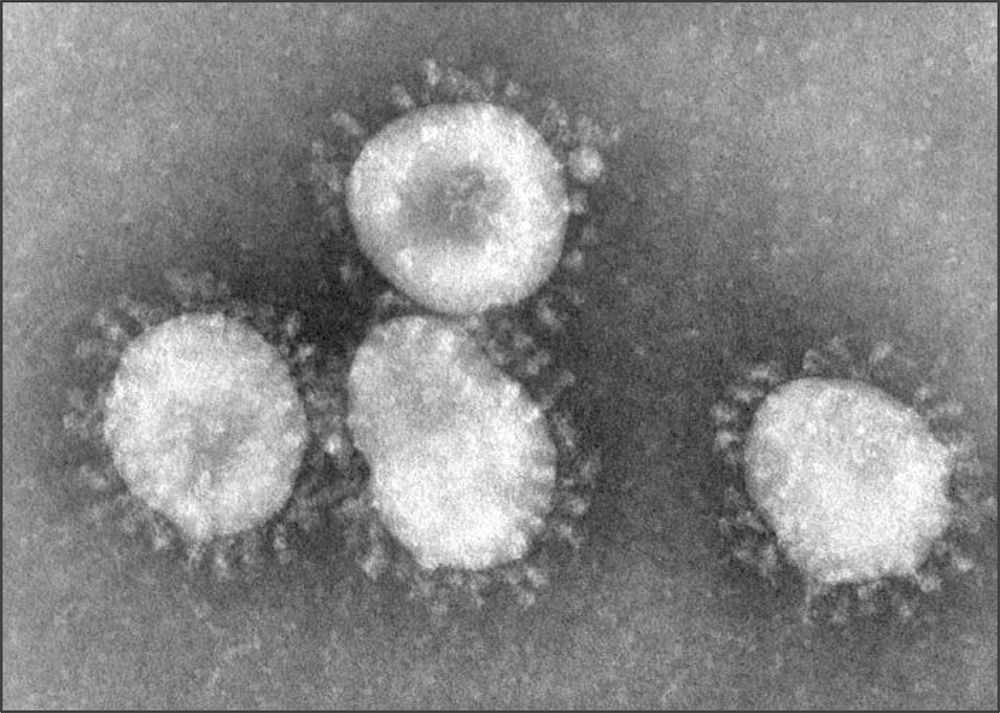
\includegraphics[width = 0.6\textwidth]{../images/coronavirus.png}
	\caption{Coronaviruses as seen under a microscope. The fuzzy blobs on the cell surface are spike proteins, which the virus uses to gain entry to host cells.}
	\label{fig:coronavirus}
\end{figure}

When viewed under a microscope, the two viruses look identical, and they use the same mechanism to infect human cells, when the spike protein on the virus surface bonds to the ACE2 enzyme on a human cell's membrane. So why did SARS fizzle, but SARS-CoV-2, a disease that is on average less harmful and less deadly to individuals who contract it, transform into a pandemic? The most likely explanation for the ability of SARS-CoV-2 to spread across far more countries and remain a public health threat even in the face of lockdowns is that it spreads more easily; that is, it is more \textdefnogloss{infectious}. Is there a molecular basis of this increased infectiousness?

We will place ourselves in the shoes of early SARS-CoV-2 researchers studying the new virus in early 2020. The virus's genome, consisting of nearly 30,000 nucleotides, was published on January 10, and an annotation of this genome showing the position of the virus's genes is shown in \autoref{fig:SARSCoV2Annotation}. Upon sequence comparison, SARS-CoV-2 was found to be related to several coronaviruses isolated from bats and distantly related to SARS-CoV.

\begin{figure}[h]
	\centering
	\mySfFamily
	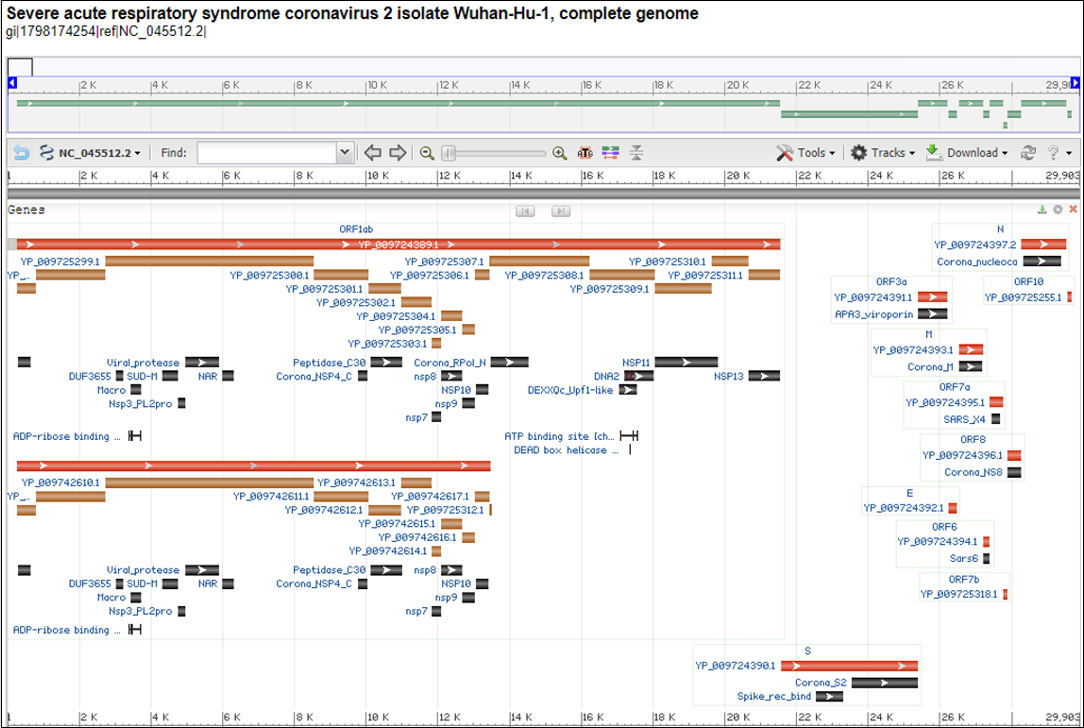
\includegraphics[width = 0.85\textwidth]{../images/SARSCoV2Annotation.png}
	\caption{An annotated genome of SARS-CoV-2. The Spike protein, found at the bottom of this image, is labeled ``S'' and begins at nucleotide position 21,563.}
	\label{fig:SARSCoV2Annotation}
\end{figure}

Recall from our discussion of transcription factors in \autoref{chapter:motifs} that by the central dogma of molecular biology, DNA is transcribed into RNA, which is then translated into protein. According to the genetic code, triplets of RNA nucleotides called codons are converted into single amino acids. The resulting chain of amino acids is called a \textdef{polypeptide}{polypeptide}{a linear chain of amino acids that forms part or all of a protein}.

The gene encoding the spike protein starts at nucleotide position 21,563 of the SARS-CoV-2 genome, and the corresponding translated polypeptide chain is shown in \autoref{fig:spike_protein_sequence}. Each of 20 possible amino acids is represented by a letter taken from the Latin alphabet (all letters except for ``B'', ``J'', ``O'', ``U'', ``X'', and ``Z'' are used for amino acids). As you examine the string of letters in this figure, consider how global mayhem can ultimately be caused by something so tiny.

\begin{figure}[h]
\begin{ttsequence}[0.93]MFVFLVLLPLVSSQCVNLTTRTQLPPAYTNSFTRGVYYPDKVFRSSVLHSTQDLFLPFFSNVTWFHAIHV\\
SGTNGTKRFDNPVLPFNDGVYFASTEKSNIIRGWIFGTTLDSKTQSLLIVNNATNVVIKVCEFQFCNDPF\\
LGVYYHKNNKSWMESEFRVYSSANNCTFEYVSQPFLMDLEGKQGNFKNLREFVFKNIDGYFKIYSKHTPI\\
NLVRDLPQGFSALEPLVDLPIGINITRFQTLLALHRSYLTPGDSSSGWTAGAAAYYVGYLQPRTFLLKYN\\
ENGTITDAVDCALDPLSETKCTLKSFTVEKGIYQTSNFRVQPTESIVRFPNITNLCPFGEVFNATRFASV\\
YAWNRKRISNCVADYSVLYNSASFSTFKCYGVSPTKLNDLCFTNVYADSFVIRGDEVRQIAPGQTGKIAD\\
YNYKLPDDFTGCVIAWNSNNLDSKVGGNYNYLYRLFRKSNLKPFERDISTEIYQAGSTPCNGVEGFNCYF\\
PLQSYGFQPTNGVGYQPYRVVVLSFELLHAPATVCGPKKSTNLVKNKCVNFNFNGLTGTGVLTESNKKFL\\
PFQQFGRDIADTTDAVRDPQTLEILDITPCSFGGVSVITPGTNTSNQVAVLYQDVNCTEVPVAIHADQLT\\
PTWRVYSTGSNVFQTRAGCLIGAEHVNNSYECDIPIGAGICASYQTQTNSPRRARSVASQSIIAYTMSLG\\
AENSVAYSNNSIAIPTNFTISVTTEILPVSMTKTSVDCTMYICGDSTECSNLLLQYGSFCTQLNRALTGI\\
AVEQDKNTQEVFAQVKQIYKTPPIKDFGGFNFSQILPDPSKPSKRSFIEDLLFNKVTLADAGFIKQYGDC\\
LGDIAARDLICAQKFNGLTVLPPLLTDEMIAQYTSALLAGTITSGWTFGAGAALQIPFAMQMAYRFNGIG\\
VTQNVLYENQKLIANQFNSAIGKIQDSLSSTASALGKLQDVVNQNAQALNTLVKQLSSNFGAISSVLNDI\\
LSRLDKVEAEVQIDRLITGRLQSLQTYVTQQLIRAAEIRASANLAATKMSECVLGQSKRVDFCGKGYHLM\\
SFPQSAPHGVVFLHVTYVPAQEKNFTTAPAICHDGKAHFPREGVFVSNGTHWFVTQRNFYEPQIITTDNT\\
FVSGNCDVVIGIVNNTVYDPLQPELDSFKEELDKYFKNHTSPDVDLGDISGINASVVNIQKEIDRLNEVA\\
KNLNESLIDLQELGKYEQYIKWPWYIWLGFIAGLIAIVMVTIMLCCMTSCCSCLKGCCSCGSCCKFDEDD\\
SEPVLKGVKLHYT\phantom{QCVNLTTRTQLPPAYTNSFTRGVYYPDKVFRSSVLHSTQDLFLPFFSNVTWFHAIHV}
\end{ttsequence}
\caption{The 1,273 amino acid sequence of the SARS-CoV-2 spike protein. Each symbol represents one of 20 amino acids.}
\label{fig:spike_protein_sequence}
\end{figure}

\phantomsection
\subsection{Nature's magic protein folding algorithm}

After the SARS-CoV-2 spike protein polypeptide chain is formed, it will ``fold'' into a three-dimensional shape. This folding process occurs spontaneously for all proteins and without any outside influence, and the same polypeptide chain will almost always fold into the same 3-D structure in a manner of microseconds. This means that nature applies some ``magic algorithm'' to produce the folded structure of a protein from its sequence of amino acids.

Predicting the folded structure of a polypeptide is called \textdef{protein structure prediction}{protein structure prediction}{the problem of predicting the folded three-dimensional structure of a polypeptide from its nucleotide sequence}, and this problem is simple to state but deceptively difficult to solve. In fact, it has been an active area of biological research for several decades.

Why do we care about protein structure? Knowing a protein's structure is essential to determining its function and how it interacts with other proteins or molecules in its environment. Determining protein function is still an active area of research: we still do not know the function of a few thousand human genes, and \autoref{fig:different_protein_shapes_2020} shows the huge variety of protein shapes in the 2020 ``proteins of the month'' named by the \textdef{Protein Data Bank (PDB)}{Protein Data Bank (PDB)}{a public database for the structural study of proteins}. (Note that the June 2020 winner is the SARS-CoV-2 spike protein.)

\begin{figure}[h]
	\centering
	\mySfFamily
	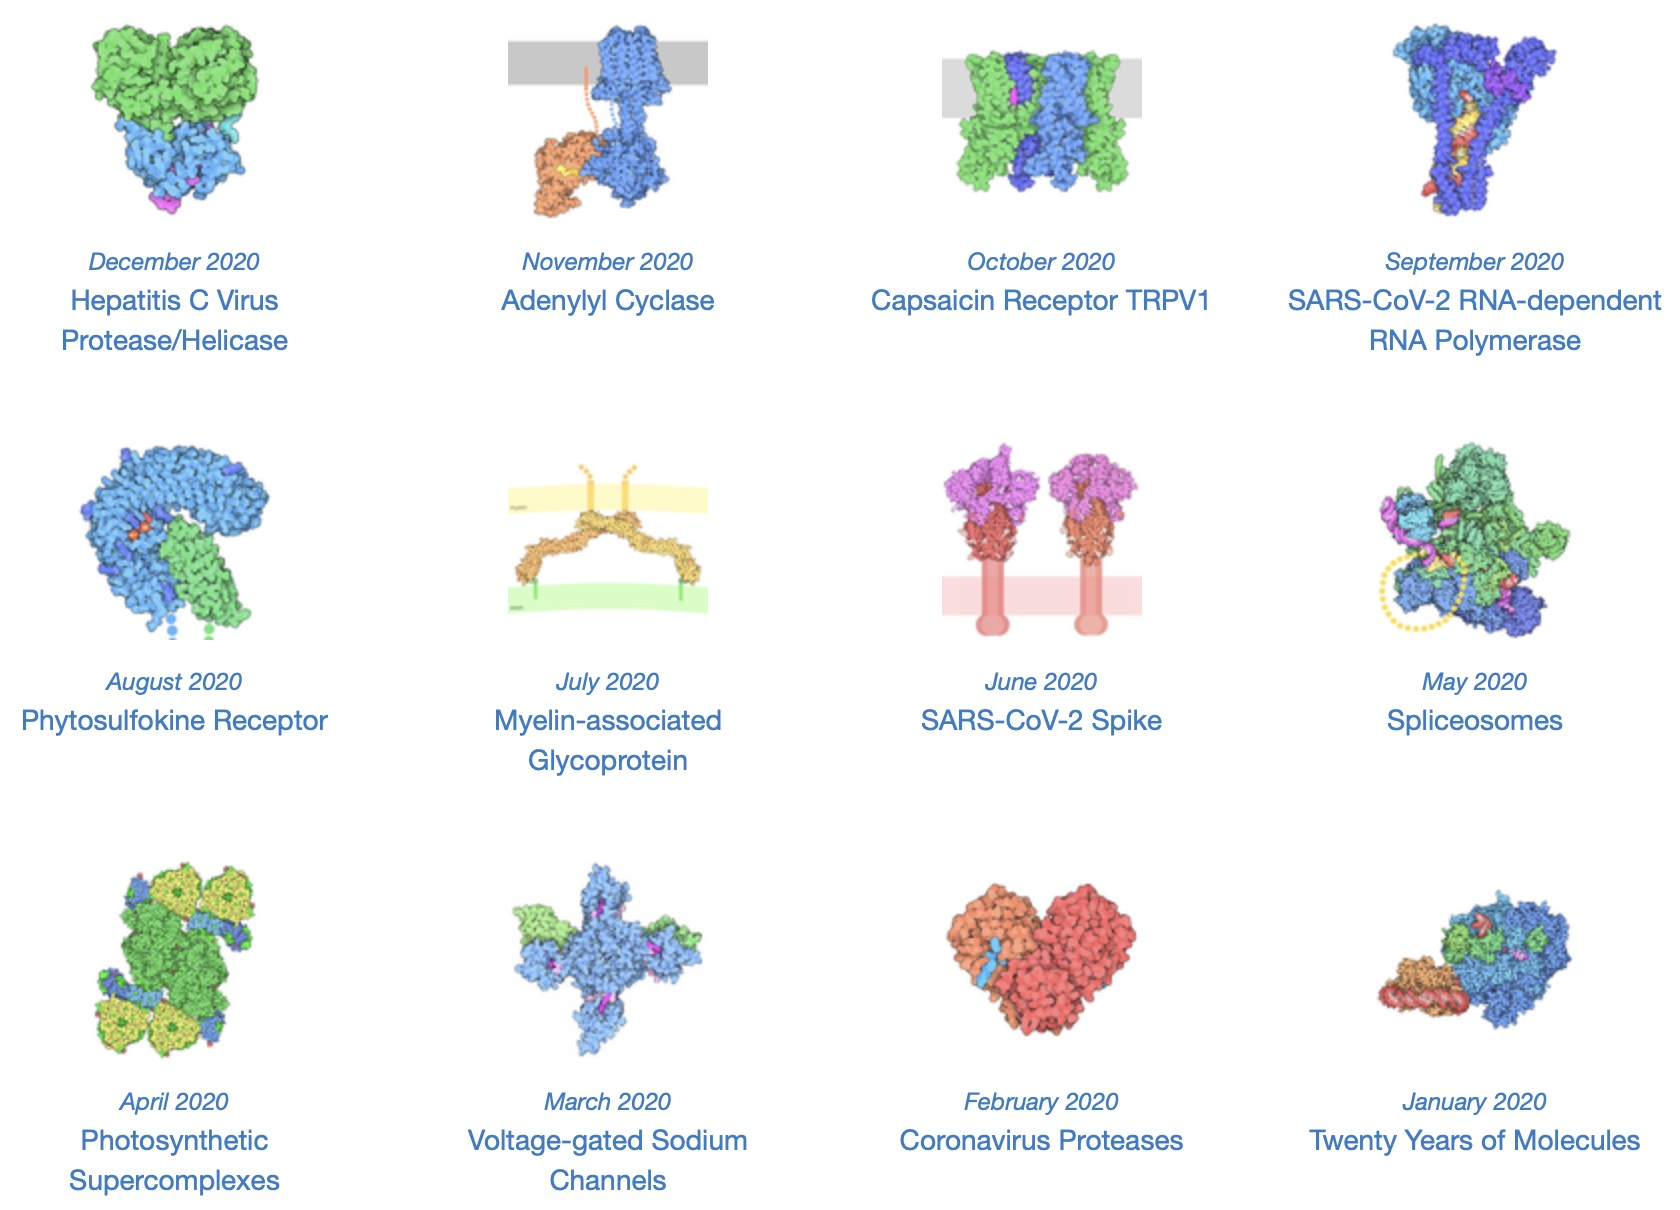
\includegraphics[width = 0.85\textwidth]{../images/different_protein_shapes_2020.jpg}
	\caption{Each ``molecule of the month'' in 2020 named by the PDB. These proteins have widely varying shapes and accomplish a wide variety of cellular tasks. The SARS-CoV-2 spike protein was the molecule of the month in June.}
	\label{fig:different_protein_shapes_2020}
\end{figure}

Another central problem in protein structural research is devoted to understanding protein interactions. For example, a disease may be caused by a faulty protein, in which case researchers want to find a drug that binds to the protein and causes some change of interest in that protein, such as inhibiting its behavior.

In our work with SARS-CoV-2 spike protein analysis, we will consider two questions. First, can we reverse engineer nature's magic algorithm and determine the spike protein's shape from its sequence of amino acids in \autoref{fig:spike_protein_sequence}? Second, once we know this molecular structure of the SARS-CoV-2 spike protein, how does its structure and function differ from the same protein in SARS-CoV?

These two questions are both significant, and so we will split our work on them over two chapters. If you are already familiar with protein structure prediction, then you may want to skip ahead to \autoref{chapter:coronavirus_2}, in which we discuss how to identify structural differences between the spike proteins of the two viruses.\\

\FloatBarrier
\phantomsection

\section{Protein Structure Prediction is Difficult}
\label{sec:structure_intro}

\phantomsection
\subsection{Experimental methods for determining protein structure}

Although we would like to infer nature's magic algorithm for inferring protein structure from amino acid sequence, biochemists can determine the structure of a protein experimentally. In \textdef{X-ray crystallography}{X-ray crystallography}{an experimental process in which researchers crystallize many copies of a molecule such as a protein and then shine an intense beam of X-rays at the crystal in order to determine the molecule's structure}, researchers crystallize many copies of a protein and then shine an intense beam of X-rays at the crystal. The light hitting the protein is diffracted, creating patterns from which the position of every atom in the protein can be inferred.

X-ray crystallography is over a century old and has been the \textit{de facto} approach for protein structure determination for decades. Yet a newer method is now rapidly replacing X-ray crystallography. In \textdef{cryo-electron microscopy (cryo-EM)}{cryo-electron microscopy (cryo-EM)}{an experimental process in which researchers preserve thousands of copies of a molecule such as a protein in non-crystalline ice and then examine these copies with an electron microscope}, researchers preserve thousands of copies of a protein in non-crystalline ice and then examine these copies with an electron microscope.

Unfortunately, laboratory approaches for structure determination are expensive and cannot be used on all proteins. An X-ray crystallography experiment for a single protein costs upward of \$2,000, and building an electron microscope can cost millions of dollars. When applying X-ray crystallography, crystallizing a protein is a challenging task, and each copy of the protein must line up in the same way, which does not work for very flexible proteins  And to study bacterial proteins, we need to culture the bacteria in the lab, but microbiologists have estimated that less than 2\% of bacteria can be cultured with current approaches.

Protein structures that have been determined experimentally are typically stored in the PDB, which contains over 160,000 protein structures. This number may seem large, but a recent study estimated that the 20,000 human genes translate into between 620,000 and 6.13 million protein isoforms (i.e., protein variants with slightly different structures). If we hope to catalog the proteins of all living things, then our work on structure determination is just beginning.

\FloatBarrier
\phantomsection
\subsection{Protein sequence and structure do not correlate well}

Predicting protein structure from amino acid sequence is very challenging. On the one hand, small perturbations in the sequence of a protein can drastically change the protein's shape and even render it useless; sickle cell anemia is caused by a single amino acid mutation in hemoglobin subunit beta that causes hemoglobin molecules to bind into long chains, which winds up altering the shape of the red blood cells carrying hemoglobin. On the other hand, different amino acids can have similar chemical properties, and so some mutations will hardly change the shape of the protein. As a result, two very different amino acid sequences can fold into proteins with similar structure and comparable function.

For example, \autoref{fig:SequenceStructureExample} compares the sequences and structures of hemoglobin subunit alpha taken from three species: humans, shortfin mako sharks, and emus. Hemoglobin is the oxygen-transport protein in the blood, consisting of two alpha ``subunit'' proteins and two beta subunit proteins that combine into a protein complex; because hemoglobin is well-studied and much shorter than the SARS-CoV-2 spike protein (the alpha and beta subunits are only 140 and 146 amino acids long, respectively), we will use it as an example throughout this chapter. The alpha subunits for the three species are markedly different in terms of amino acid sequence, and yet their structures are essentially identical.\\

\begin{figure}[h]
	\centering
	\mySfFamily
	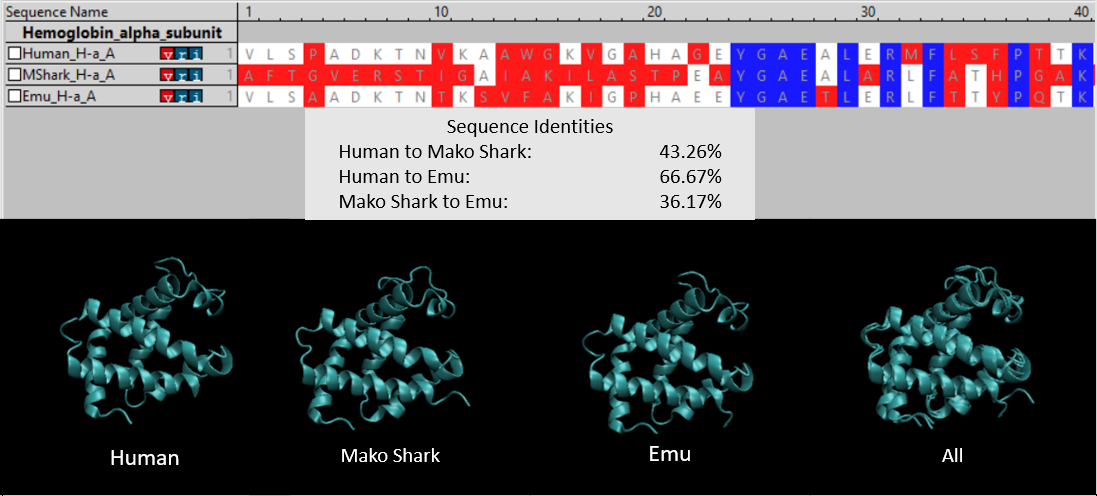
\includegraphics[width = 0.85\textwidth]{../images/SequenceStructureExample.png}
	\caption{(Top) An amino acid sequence comparison of the first 40 (out of 140) amino acids of hemoglobin subunit alpha for three species: human (PDB entry: 1si4), shortfin mako shark (PDB entry: 3mkb), and emu (PDB entry: 3wtg). A column is colored blue if all three species have the same amino acid, white if two species have the same amino acid, and red if all amino acids are different. Sequence identity calculates the number of positions in two amino acid sequences that share the same amino acid. (Bottom) Side by side comparisons of the 3-D structures of the three proteins. The final figure on the right superimposes the first three structures to highlight their similarities.}
	\label{fig:SequenceStructureExample}
\end{figure}

\phantomsection
\subsection{Flexible polypeptide chains can fold into many possible structures}

Another reason why protein structure prediction is so difficult is because a polypeptide is very flexible, with the ability to rotate in multiple ways at each amino acid, which means that the polypeptide is able to fold into a staggering number of different shapes. This polypeptide flexibility owes to the molecular structure of amino acids. As shown in \autoref{fig:AminoAcid}, an amino acid comprises four parts. In the center, a carbon atom (called the \textdef{alpha carbon}{alpha carbon}{the central carbon atom of an amino acid}) is connected to four different molecules: a hydrogen atom (H), a \textdefnogloss{carboxyl group} ($-\text{COOH}$), an \textdefnogloss{amino group} ($-\text{NH}_2$), and a \textdefnogloss{side chain} (denoted ``R'' and often called an \textbf{R group}). The side chain is a molecule that differs between different amino acids and ranges in mass from a single hydrogen atom (glycine) up to $-\text{C}_8\text{H}_7\text{N}$ (tryptophan).\\

\begin{figure}[h]
	\centering
	\mySfFamily
	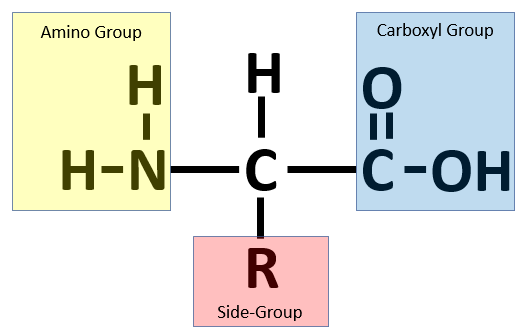
\includegraphics[width = 0.4\textwidth]{../images/AminoAcid.png}
	\caption{An amino acid consists of a central, alpha carbon attached to a hydrogen atom, a side group, a carboxyl group, and an amino group.}
	\label{fig:AminoAcid}
\end{figure}

To form a polypeptide chain, consecutive amino acids are linked together during a condensation reaction in which the amino group of one amino acid is joined to the carboxyl group of another, while a water molecule ($\text{H}_2\text{O}$) is expelled (\autoref{fig:condensation} (top)). The resulting bond that is produced between the carbon atom of one amino acid's carboxyl group and the nitrogen atom of the next amino acid's amino group, called a \textdefnogloss{peptide bond}, is very strong. The peptide has very little rotation around this bond, which is almost always locked at 180\textdegree. As peptide bonds are formed between adjacent amino acids, the polypeptide chain takes shape (\autoref{fig:condensation} (bottom)).

\begin{figure}[h]
	\centering
	\mySfFamily
	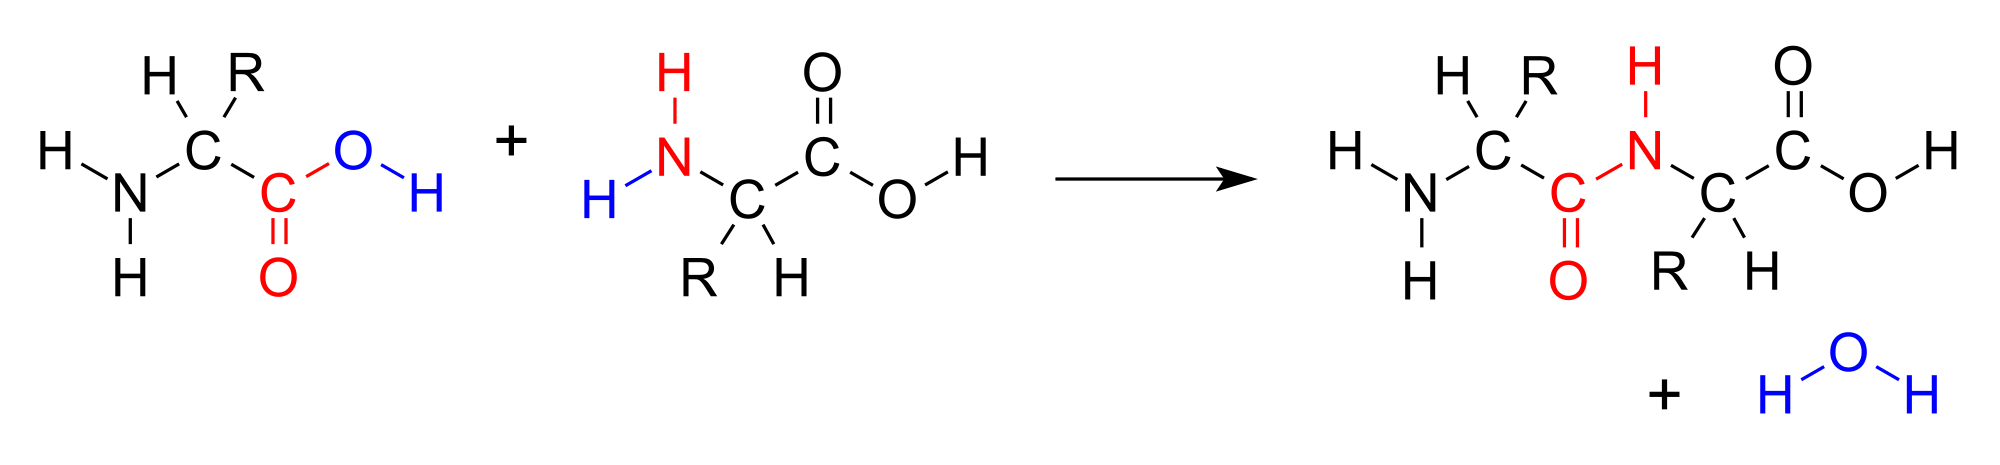
\includegraphics[width = 0.85\textwidth]{../images/dipeptide_reaction.png}\\[0.5ex]
	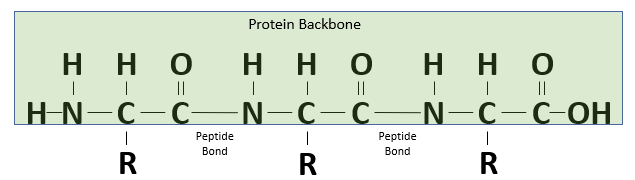
\includegraphics[width = 0.6\textwidth]{../images/Backbone.png}
	\caption{(Top) A condensation reaction joins two amino acids into a ``dipeptide'' by joining the amino group of one amino acid to the carboxyl group of the other, with a water molecule expelled. (Bottom) A protein backbone formed of three amino acids.}
	\label{fig:condensation}
\end{figure}

However, the bonds \textit{within} an amino acid, joining the alpha carbon to its carboxyl group and amino group, are not as rigid, and the polypeptide is free to rotate around these two bonds. This rotation produces two angles of interest, called the \textdefnogloss{phi angle} ($\phi$) and \textdefnogloss{psi angle} ($\psi$) (\autoref{fig:torsion_angles}), which are formed at the alpha carbon's connections to its amino group and carboxyl group, respectively.

\begin{figure}[b]
	\centering
	\mySfFamily
	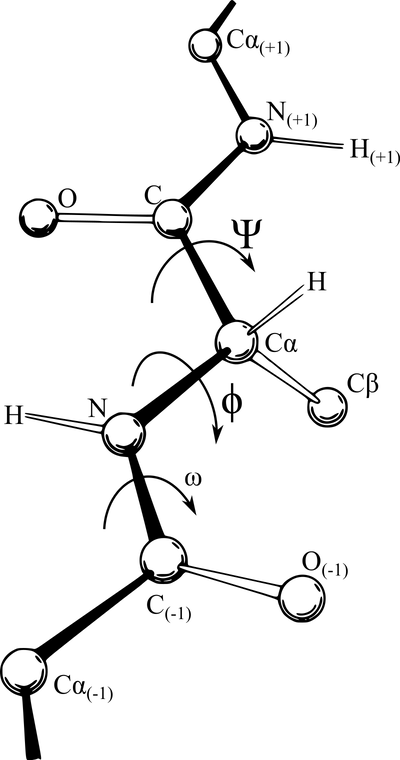
\includegraphics[width = 0.25\textwidth]{../images/torsion_angles.png}
	\caption{A polypeptide chain of multiple amino acids with the torsion angles $\phi$ and $\psi$ indicated. The angle ω indicates the angle of the peptide bond, which is typically 180\textdegree.}
	\label{fig:torsion_angles}
\end{figure}

A good analogy for polypeptide flexibility is the ``Rubik's Twist'' puzzle, which consists of a linear chain of flexible blocks that can form many different shapes. \autoref{fig:rubiks_twist_four_panel} shows the Rubik's Twist folding into a ball.

\begin{figure}[h]
	\centering
	\mySfFamily
	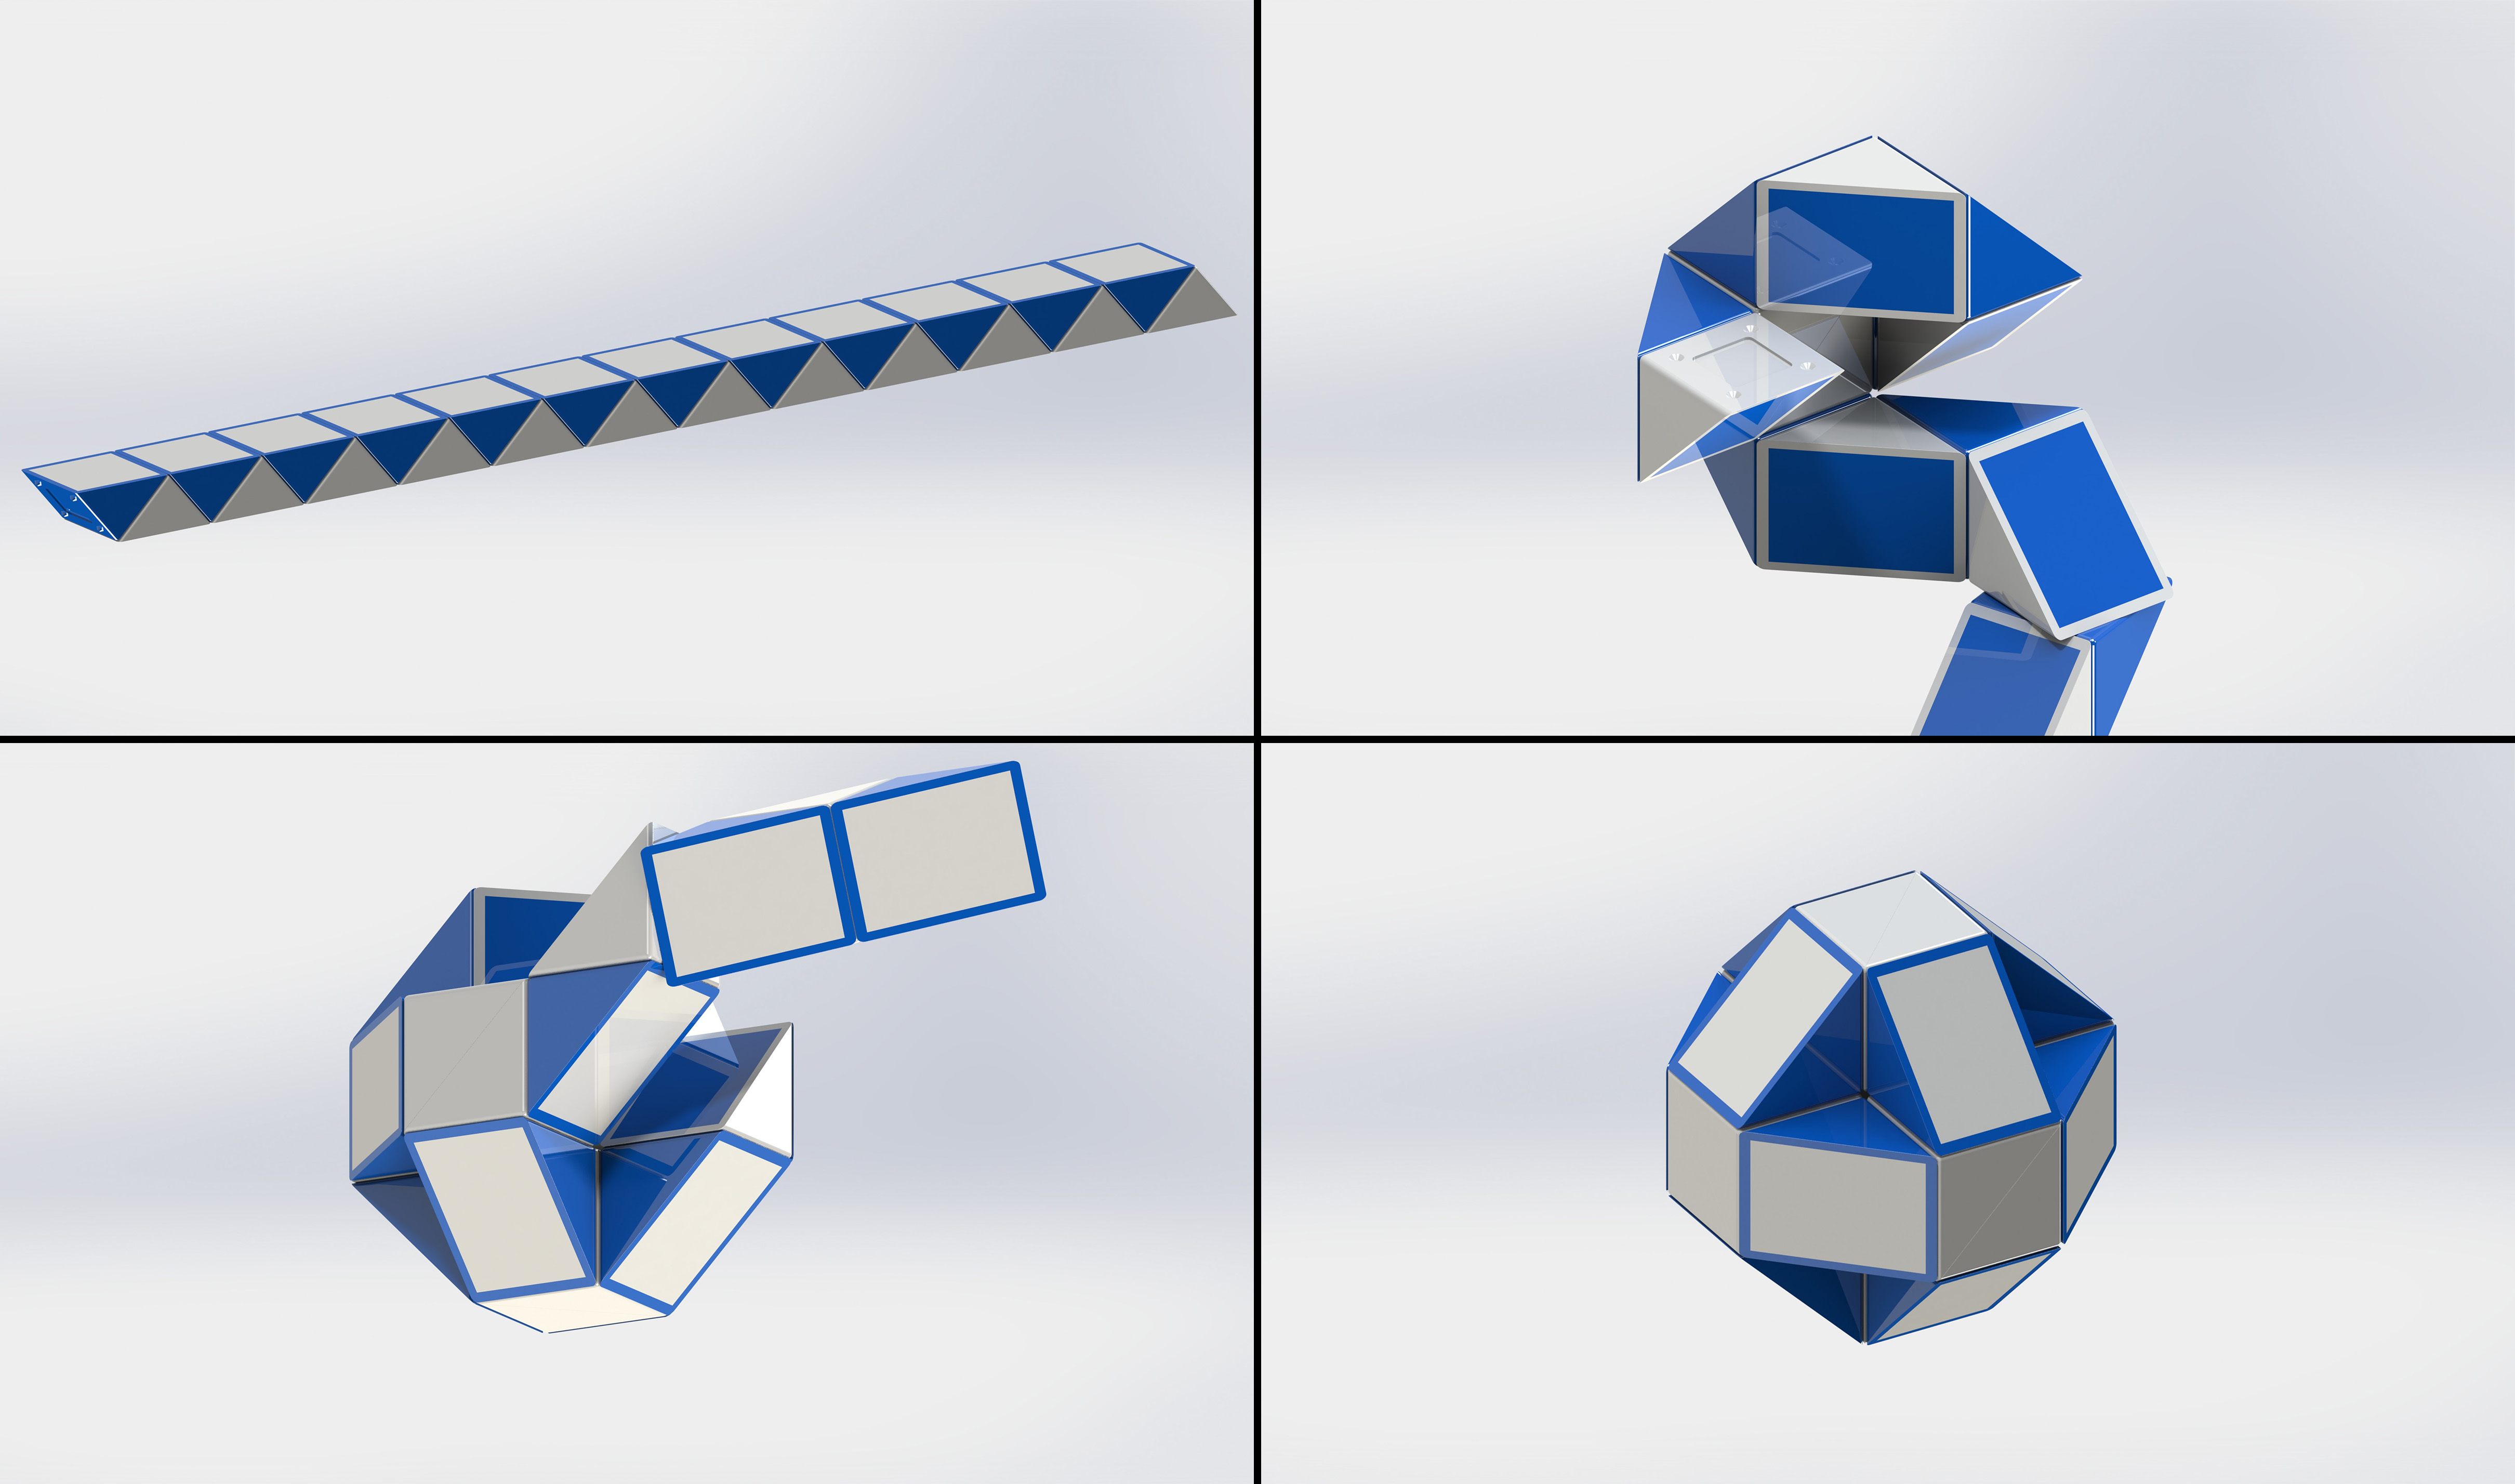
\includegraphics[width = 0.85\textwidth]{../images/rubiks_twist_four_panel.jpg}
	\caption{Each section of the Rubik's Twist puzzle can be rotated, allowing the toy to take on many different conformations such as a ball.}
	\label{fig:rubiks_twist_four_panel}
\end{figure}

A polypeptide with \textit{n} amino acids will have $n - 1$ peptide bonds, meaning that its shape is influenced by $n - 1$ phi angles and $n - 1$ psi angles. If each bond has \textit{k} stable conformations, then the polypeptide has $k^{2n-2}$ total possible conformations. If \textit{k} is equal to 3 and \textit{n} is equal to only 100 (representing a short polypeptide), then the number of potential protein structures is more than the number of atoms in the universe! The ability of the magic algorithm to reliably find a single conformation despite such an enormous number of potential shapes is called \textdef{Levinthal's paradox}{Levinthal's paradox}{the conundrum that a protein reliably folds into a single conformation despite there being an enormous number of potential structures for that protein}.

Although protein structure prediction is difficult, it is not impossible; the magic algorithm is not, after all, magic. But before discussing how we can solve this problem, we will need to learn a few more biochemical details and be more precise about two things. First, we should specify what we mean by the ``structure'' of a protein. Second, although we know that a polypeptide always folds into the same final three-dimensional shape, we have not said anything about \textit{why} a protein folds in a certain way. We will therefore need a better understanding of how the physicochemical properties of amino acids affect a protein's final structure.\\

\FloatBarrier
\phantomsection

\section{Protein Biochemistry}

\FloatBarrier
\phantomsection
\subsection{The four levels of protein structure}

Protein structure is a broad term that encapsulates four different levels of description. A protein's \textdef{primary structure}{primary structure}{the amino acid sequence of a polypeptide chain} refers to the amino acid sequence of the polypeptide chain, which we saw in \autoref{fig:spike_protein_sequence} for the SARS-CoV-2 spike protein.

A protein's \textdef{secondary structure}{secondary structure}{the highly regular, repeating intermediate substructures of a protein that form before the overall protein folding process completes} describes its highly regular, repeating intermediate substructures that form before the overall protein folding process completes. The two most common such substructures, shown in \autoref{fig:hemoglobin_secondary_structure}, are \textdef{alpha helices}{alpha helix}{a protein secondary structure that occurs when nearby amino acids wrap around to form a tube structure} and \textdef{beta sheets}{beta sheet}{a protein secondary structure that occurs when nearby amino acids line up side-by-side}. Alpha helices occur when nearby amino acids wrap around to form a tube structure; beta sheets occur when nearby amino acids line up side-by-side.\\

\begin{figure}[h]
	\centering
	\mySfFamily
	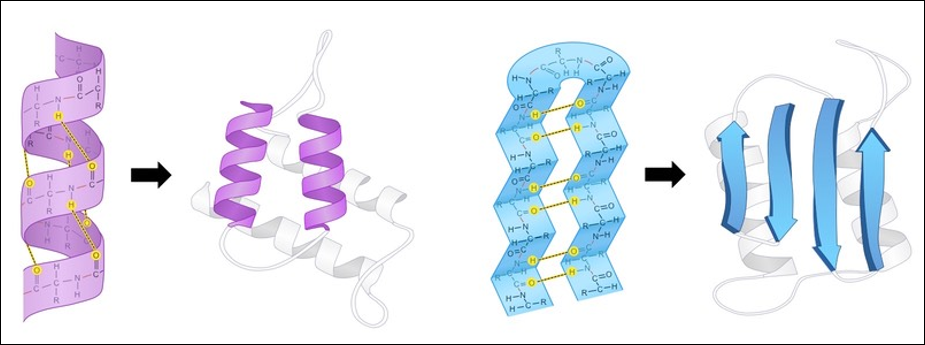
\includegraphics[width = 0.85\textwidth]{../images/hemoglobin_secondary_structure.png}
	\caption{The general shape of alpha helices (left) and beta sheets (right), the two most common protein secondary structures.}
	\label{fig:hemoglobin_secondary_structure}
\end{figure}

A protein's \textdef{tertiary structure}{tertiary structure}{the final, stable 3D shape of a protein's polypeptide chain} describes its final 3D shape after the polypeptide chain has folded and is stable. Throughout this chapter, when discussing the ``shape'' or ``structure'' of a protein, we are almost exclusively referring to its tertiary structure. \autoref{fig:hemoglobin_tertiary_structure} shows the tertiary structure of human hemoglobin subunit alpha. For the sake of simplicity, this figure does not show the position of every atom in the protein but rather represents the protein shape as a composition of secondary structures.

\begin{figure}[h]
	\centering
	\mySfFamily
	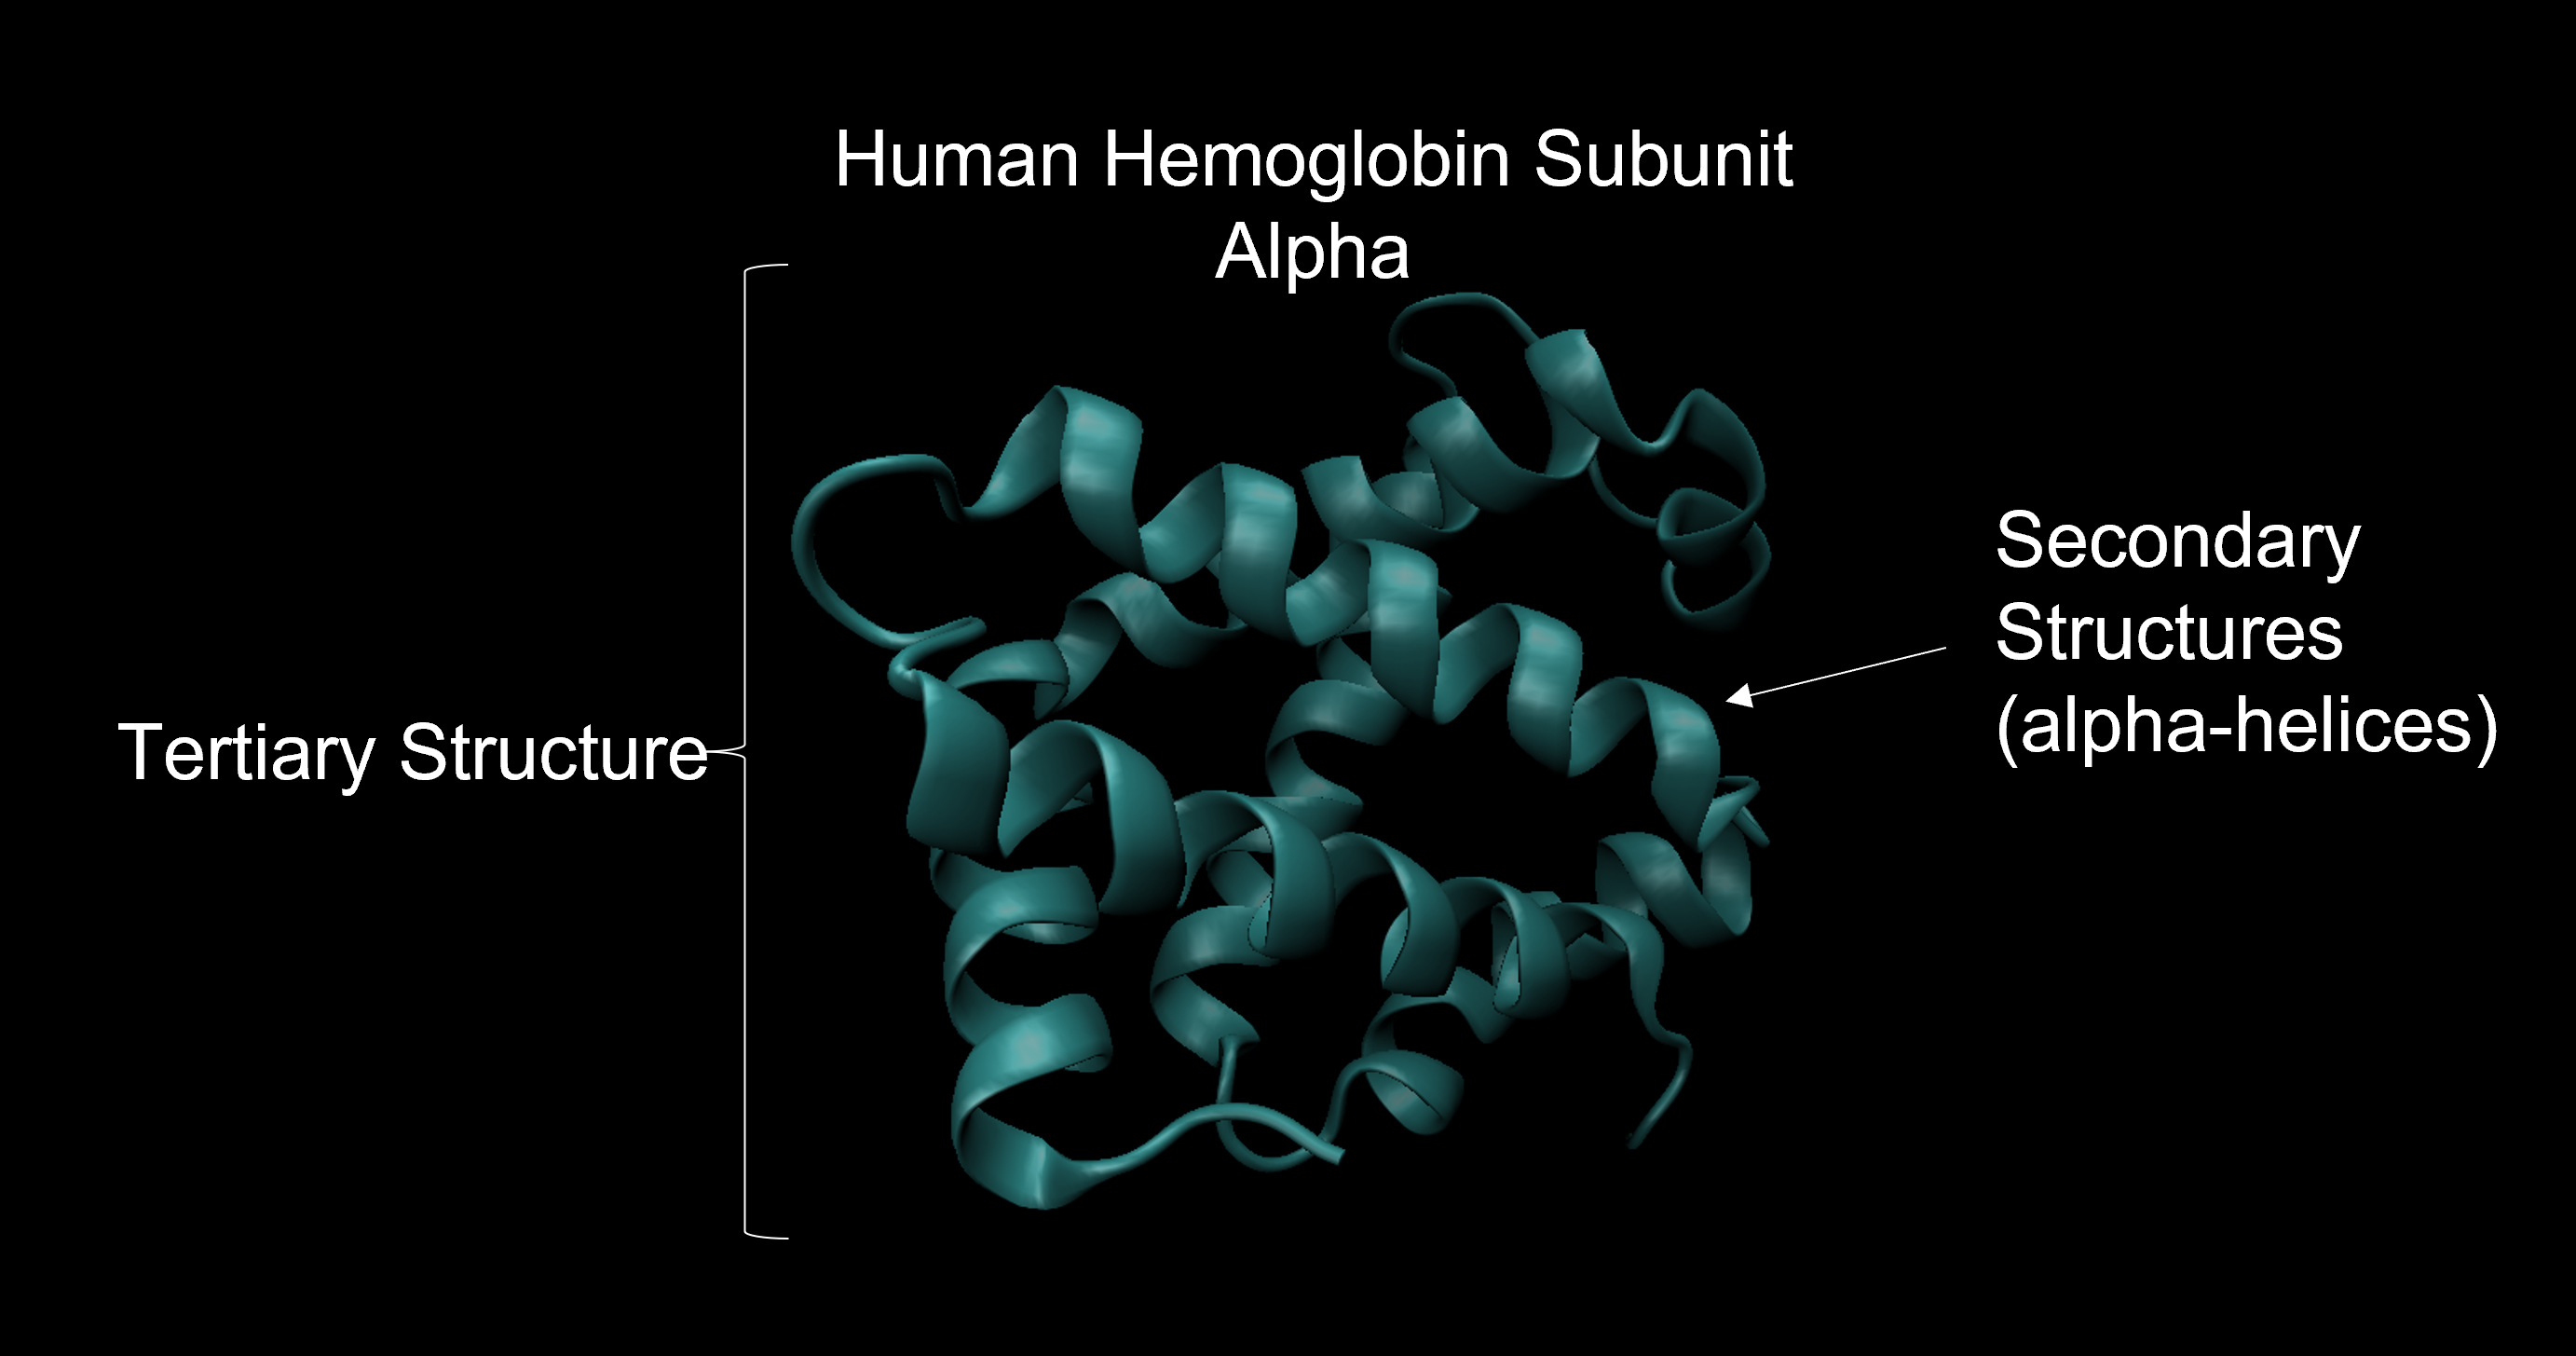
\includegraphics[width = 0.7\textwidth]{../images/hemoglobin_tertiary_structure.png}
	\caption{The tertiary structure of human hemoglobin subunit alpha. Within the structure are multiple alpha helix secondary structures.}
	\label{fig:hemoglobin_tertiary_structure}
\end{figure}

Finally, some proteins have a \textdef{quaternary structure}{quaternary structure}{the arrangement of a protein's subunits with respect to each other to form a single functional unit}, which describes the protein’s interaction with other copies of itself to form a single functional unit, or a \textdef{multimer}{multimer}{a protein formed of more than one polypeptide chain}. Many proteins do not have a quaternary structure and function as an independent monomer. \autoref{fig:quaternary_structure} (left) shows the quaternary structure of hemoglobin, which is a multimer consisting of two alpha subunits and two beta subunits.

As for SARS-CoV and SARS-CoV-2, the spike protein is a \textdefnogloss{homotrimer}, meaning that it is formed of three essentially identical units called \textdef{chains}{chain}{a subunit of a multimer}, each one translated from the corresponding region of the coronavirus's genome; these chains are colored differently in \autoref{fig:quaternary_structure} (right). In this chapter, when discussing the structure of the spike protein, we typically are referring to the structure of a single chain.

\begin{figure}[h]
	\centering
	\mySfFamily
	\tabcolsep = 1em
	\begin{tabular}{c c}
	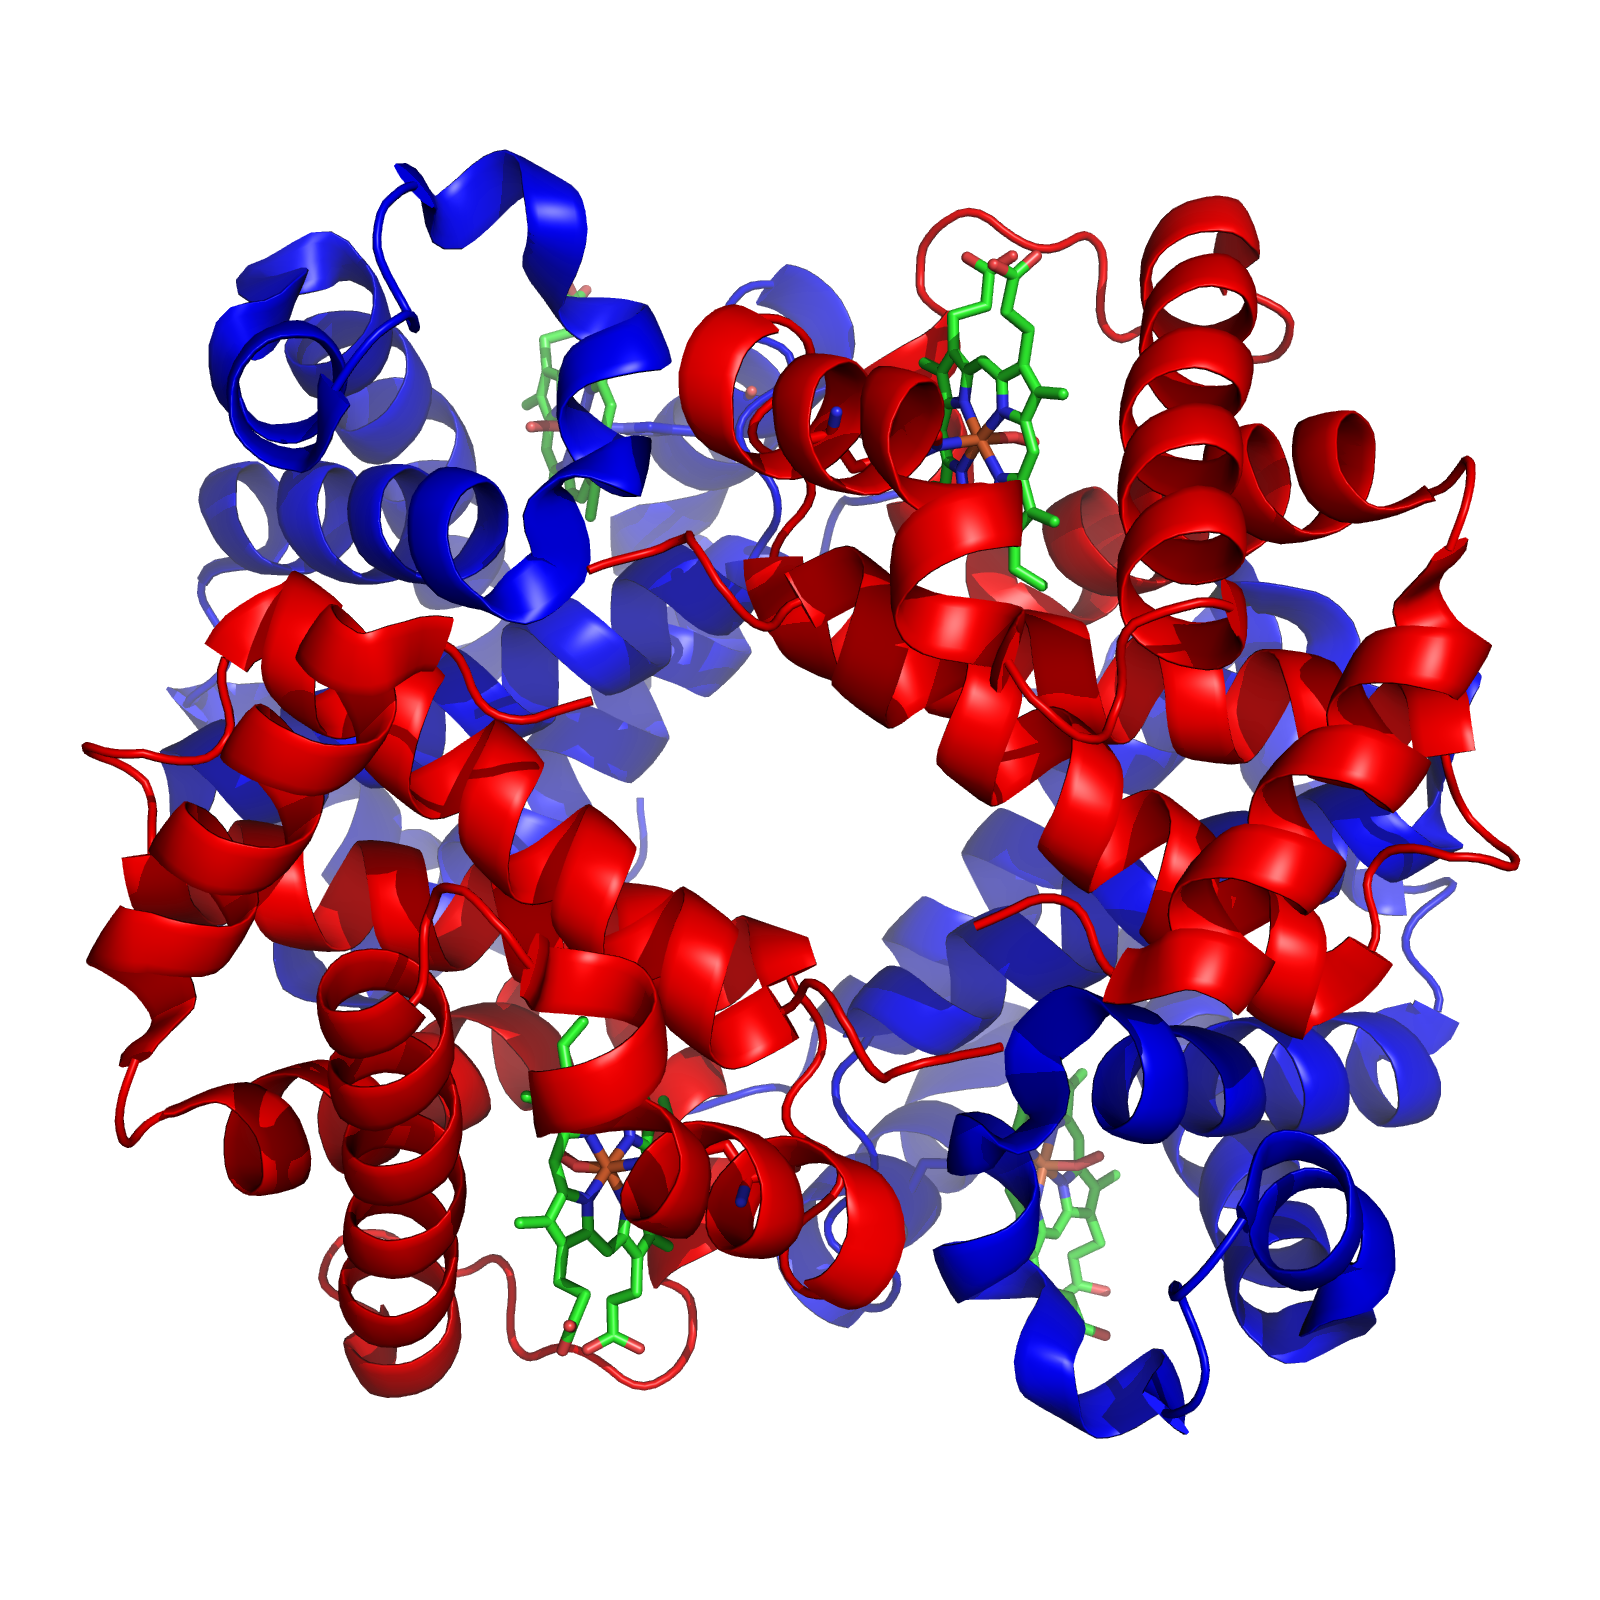
\includegraphics[width = 0.35\textwidth]{../images/hemoglobin_quaternary_structure.png} & 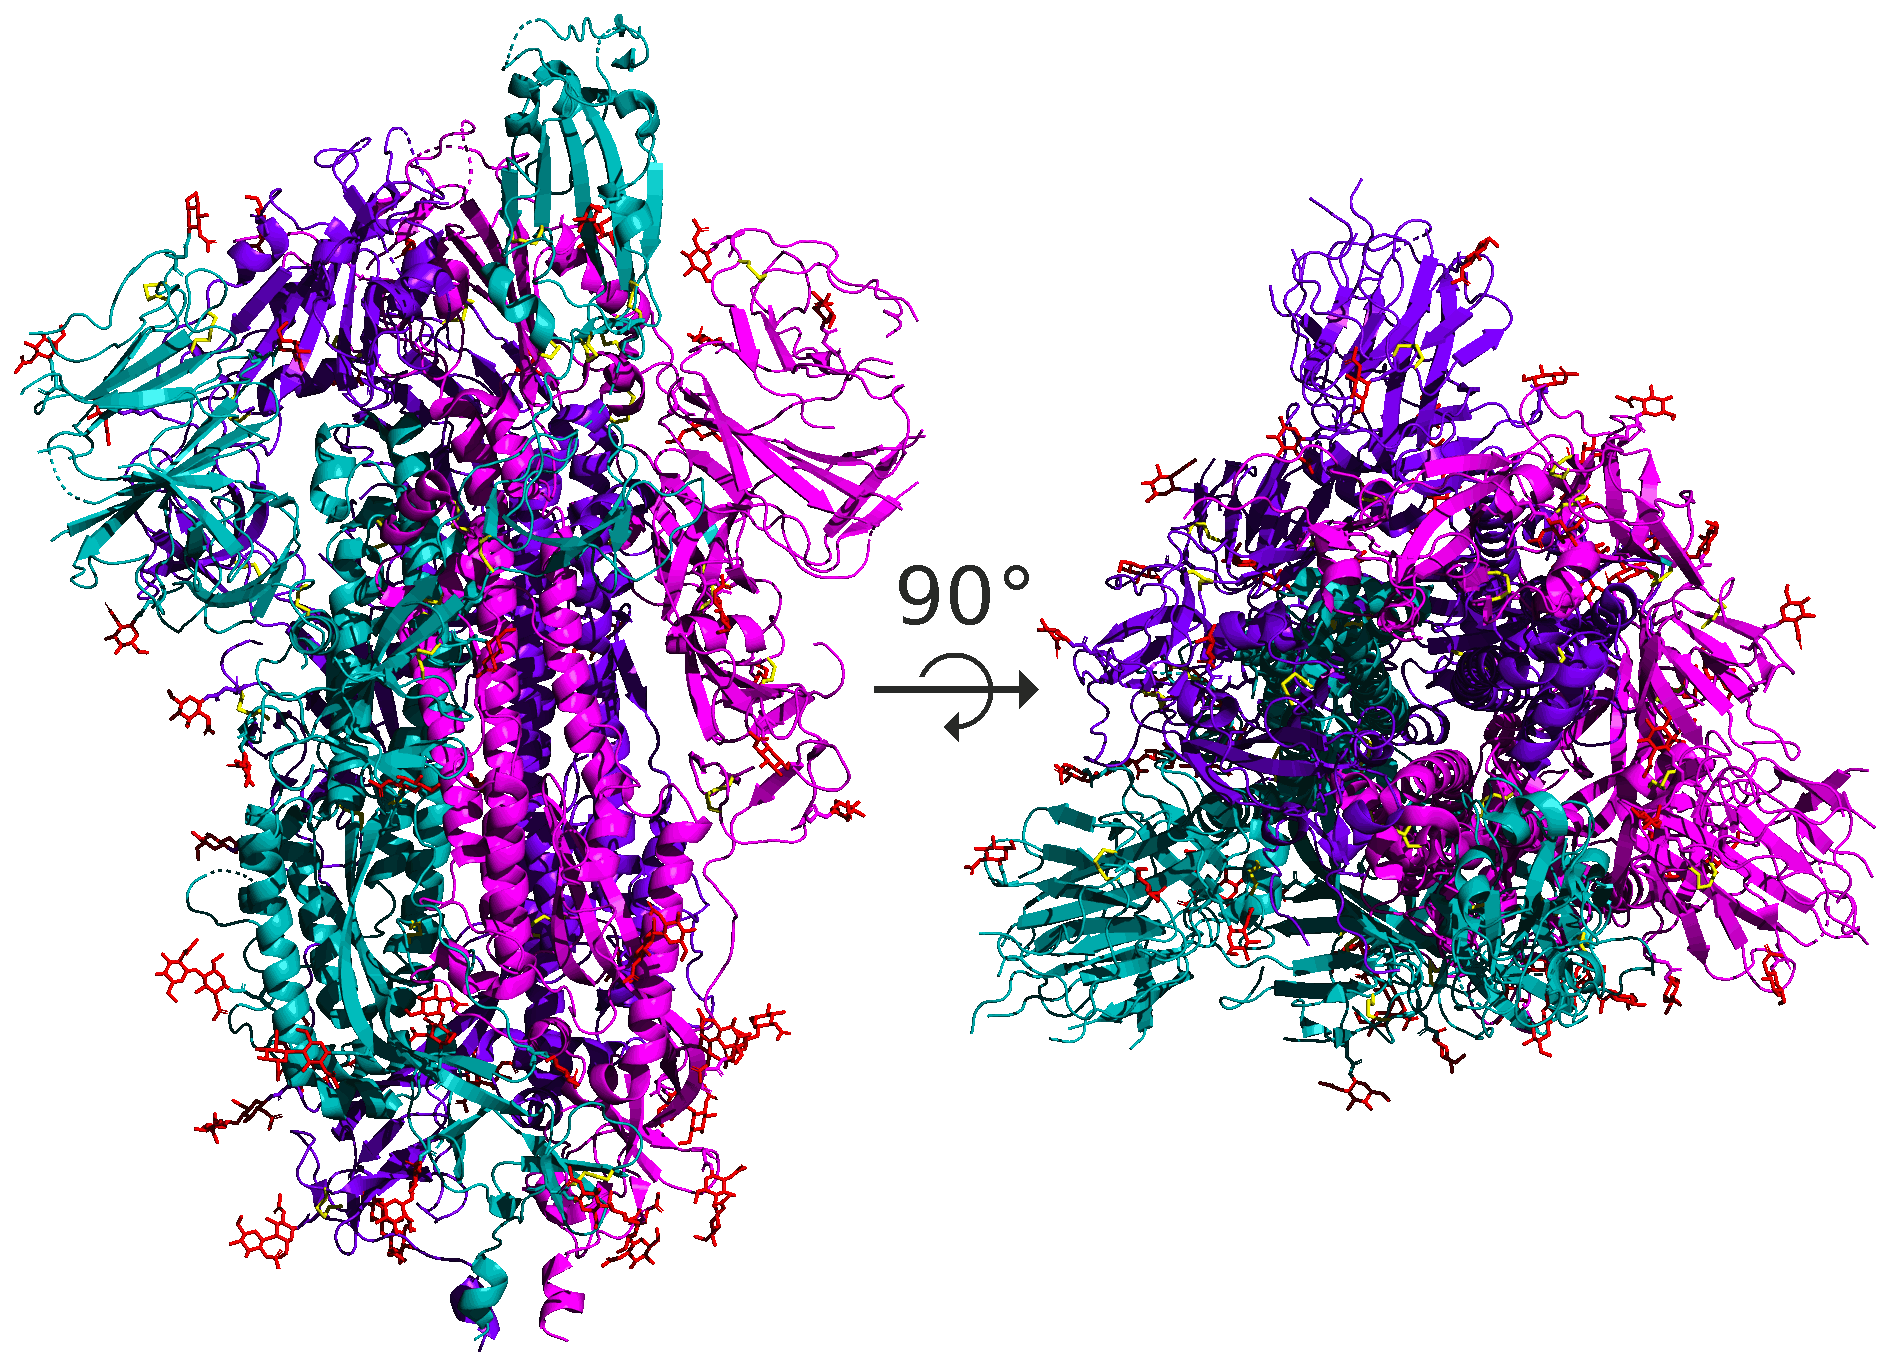
\includegraphics[width = 0.45\textwidth]{../images/spike_protein_homotrimer.png}
	\end{tabular}
	\caption{(Left) The quaternary structure of human hemoglobin, which consists of two alpha subunits (shown in red) and two beta subunits (shown in blue). Note that each alpha subunit is the tertiary structure from \autoref{fig:hemoglobin_tertiary_structure}. (Right) A side and top view of the quaternary structure of the SARS-CoV-2 spike protein homotrimer, with its three chains highlighted using different colors.}
	\label{fig:quaternary_structure}
\end{figure}

The structural units making up proteins are often hierarchical, and the spike protein is no exception. Each spike protein chain is a \textdefnogloss{dimer}, consisting of two subunits called \textdefnogloss{S1} and \textdefnogloss{S2}. Each of these subunits further divides into \textdef{protein domains}{protein domain}{a distinct structural unit within a protein that folds independently and is typically responsible for a specific interaction or function}, distinct structural units within the protein that fold independently and are typically responsible for a specific interaction or function. For example, the SARS-CoV-2 spike protein has a \textdefnogloss{receptor binding domain (RBD)} located on the S1 subunit of the spike protein that is responsible for interacting with the human ACE2 enzyme; the rest of the protein does not come into contact with ACE2. We will say more about the RBD soon.

\FloatBarrier
\subsection{Proteins seek the lowest energy conformation}

Now that we know a bit more about how protein structure is defined, we will discuss why proteins fold in the same every time. In other words, what are the factors driving the magic algorithm?

Amino acids' side chain variety causes amino acids to have different chemical properties, which can lead to different conformations being more chemically ``preferable'' than others. For example, \autoref{fig:AminoAcidChart} groups the twenty amino acids commonly occurring in proteins according to chemical properties. Nine of these amino acids are \textdefnogloss{hydrophobic} (also called \textdefnogloss{nonpolar}), meaning that their side chains tend to be repelled by water, and so we tend to find these amino acids sheltered from the environment on the interior of the protein.

\begin{figure}[h]
	\centering
	\mySfFamily
	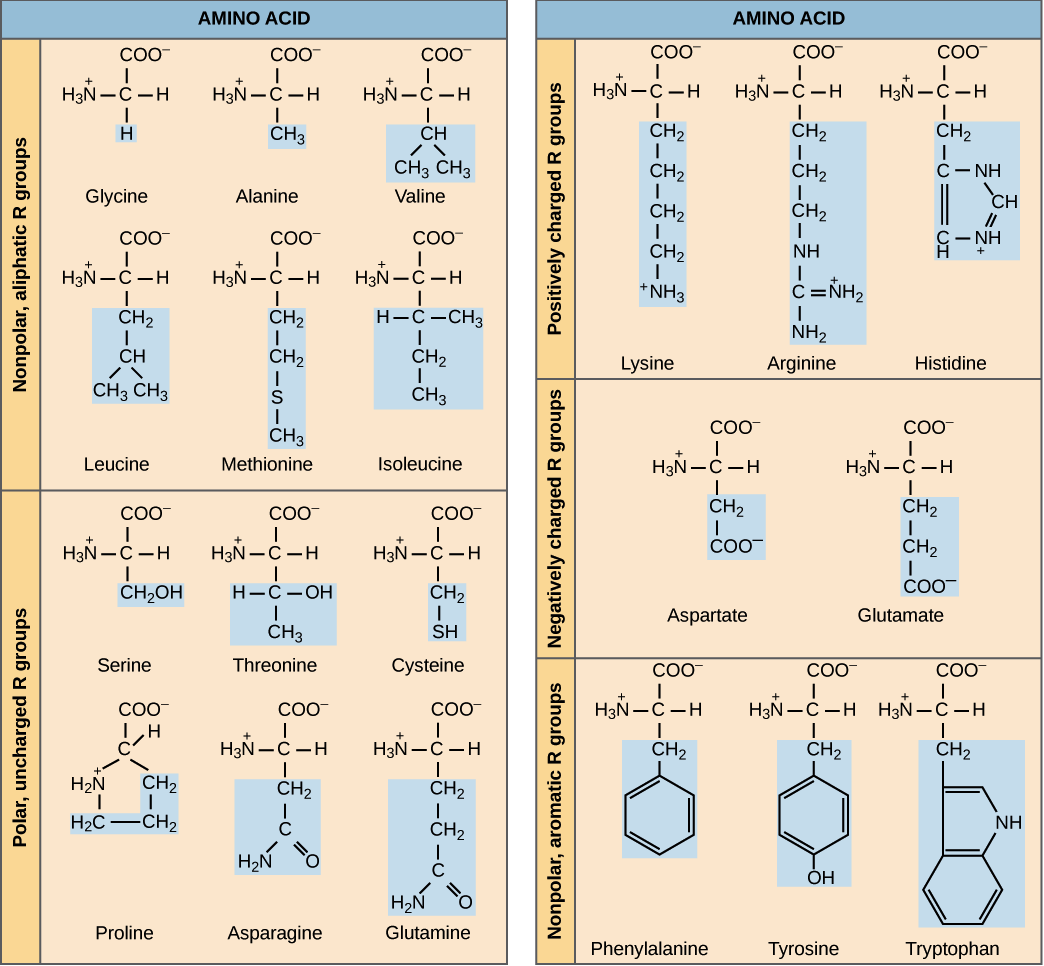
\includegraphics[width = 0.85\textwidth]{../images/AminoAcidChart.png}
	\caption{A chart of the twenty amino acid grouped by chemical properties. The side chain of each amino acid is highlighted in blue.}
	\label{fig:AminoAcidChart}
\end{figure}

We can therefore view protein folding as finding the tertiary structure that is the most \textit{stable} given a polypeptide's primary structure. A central theme of the previous chapter on bacterial chemotaxis was that a system of chemical reactions moves toward equilibrium. The same principle is true of protein folding; when a protein folds into its final structure, it is obtaining a conformation that is as chemically stable as possible.

To be more precise, the \textdef{potential energy}{potential energy}{the energy stored within a molecule due to its position, state, and arrangement, sometimes called free energy} (sometimes called \textdefnogloss{free energy}) of a molecule is the energy stored within an object due to its position, state, and arrangement. In molecular mechanics, the potential energy is made up of the sum of \textdef{bonded energy}{bonded energy}{the potential energy of a molecule deriving from the molecule's covalent bonds} and \textdef{non-bonded energy}{non-bonded energy}{the potential energy of a molecule deriving from electrostatic interactions and van der Waals interactions}.

As the protein bends and twists into a stable conformation, bonded energy derives from the protein's covalent bonds, as well as the bond angles between adjacent amino acids, and the torsion angles that we introduced earlier.

Non-bonded energy comprises \textdef{electrostatic interactions}{electrostatic interactions}{attraction and repulsion forces from electric charge between charged amino acids} and \textdef{van der Waals interactions}{van der Waals interactions}{interactions between nearby atoms due to random imbalances in the locations of electrons}. Electrostatic interactions refer to the attraction and repulsion forces from the electric charge between pairs of charged amino acids. Two of the twenty standard amino acids (arginine and lysine) are positively charged, and two (aspartic acid and glutamic acid) are negatively charged. Two nearby amino acids of opposite charge may interact to form a \textdef{salt bridge}{salt bridge}{an interaction between two nearby amino acids in a protein of opposite charge}. Conformations that contain salt bridges and keep apart similarly charged amino acids will therefore have lower free energy contributed by electrostatic interactions.

As for van der Waals interactions, atoms are dynamic systems, with electrons constantly buzzing around the nucleus. However, due to random chance, the electrons in an atom could momentarily be unevenly distributed on one side of the nucleus. Because electrons are negatively charged, this uneven distribution will cause the atom to have a temporary negative charge on the side with the excess electrons and a temporary positive charge on the opposite side. As a result of this charge, one side of the atom may attract only the oppositely charged components of another atom, creating an \textdefnogloss{induced dipole} in that atom (\autoref{fig:van_der_waals}). Van der Waals forces refer to the attraction and repulsion between atoms because of induced dipoles.\\

%\begin{figure}[h]
%	\centering
%	\mySfFamily
%	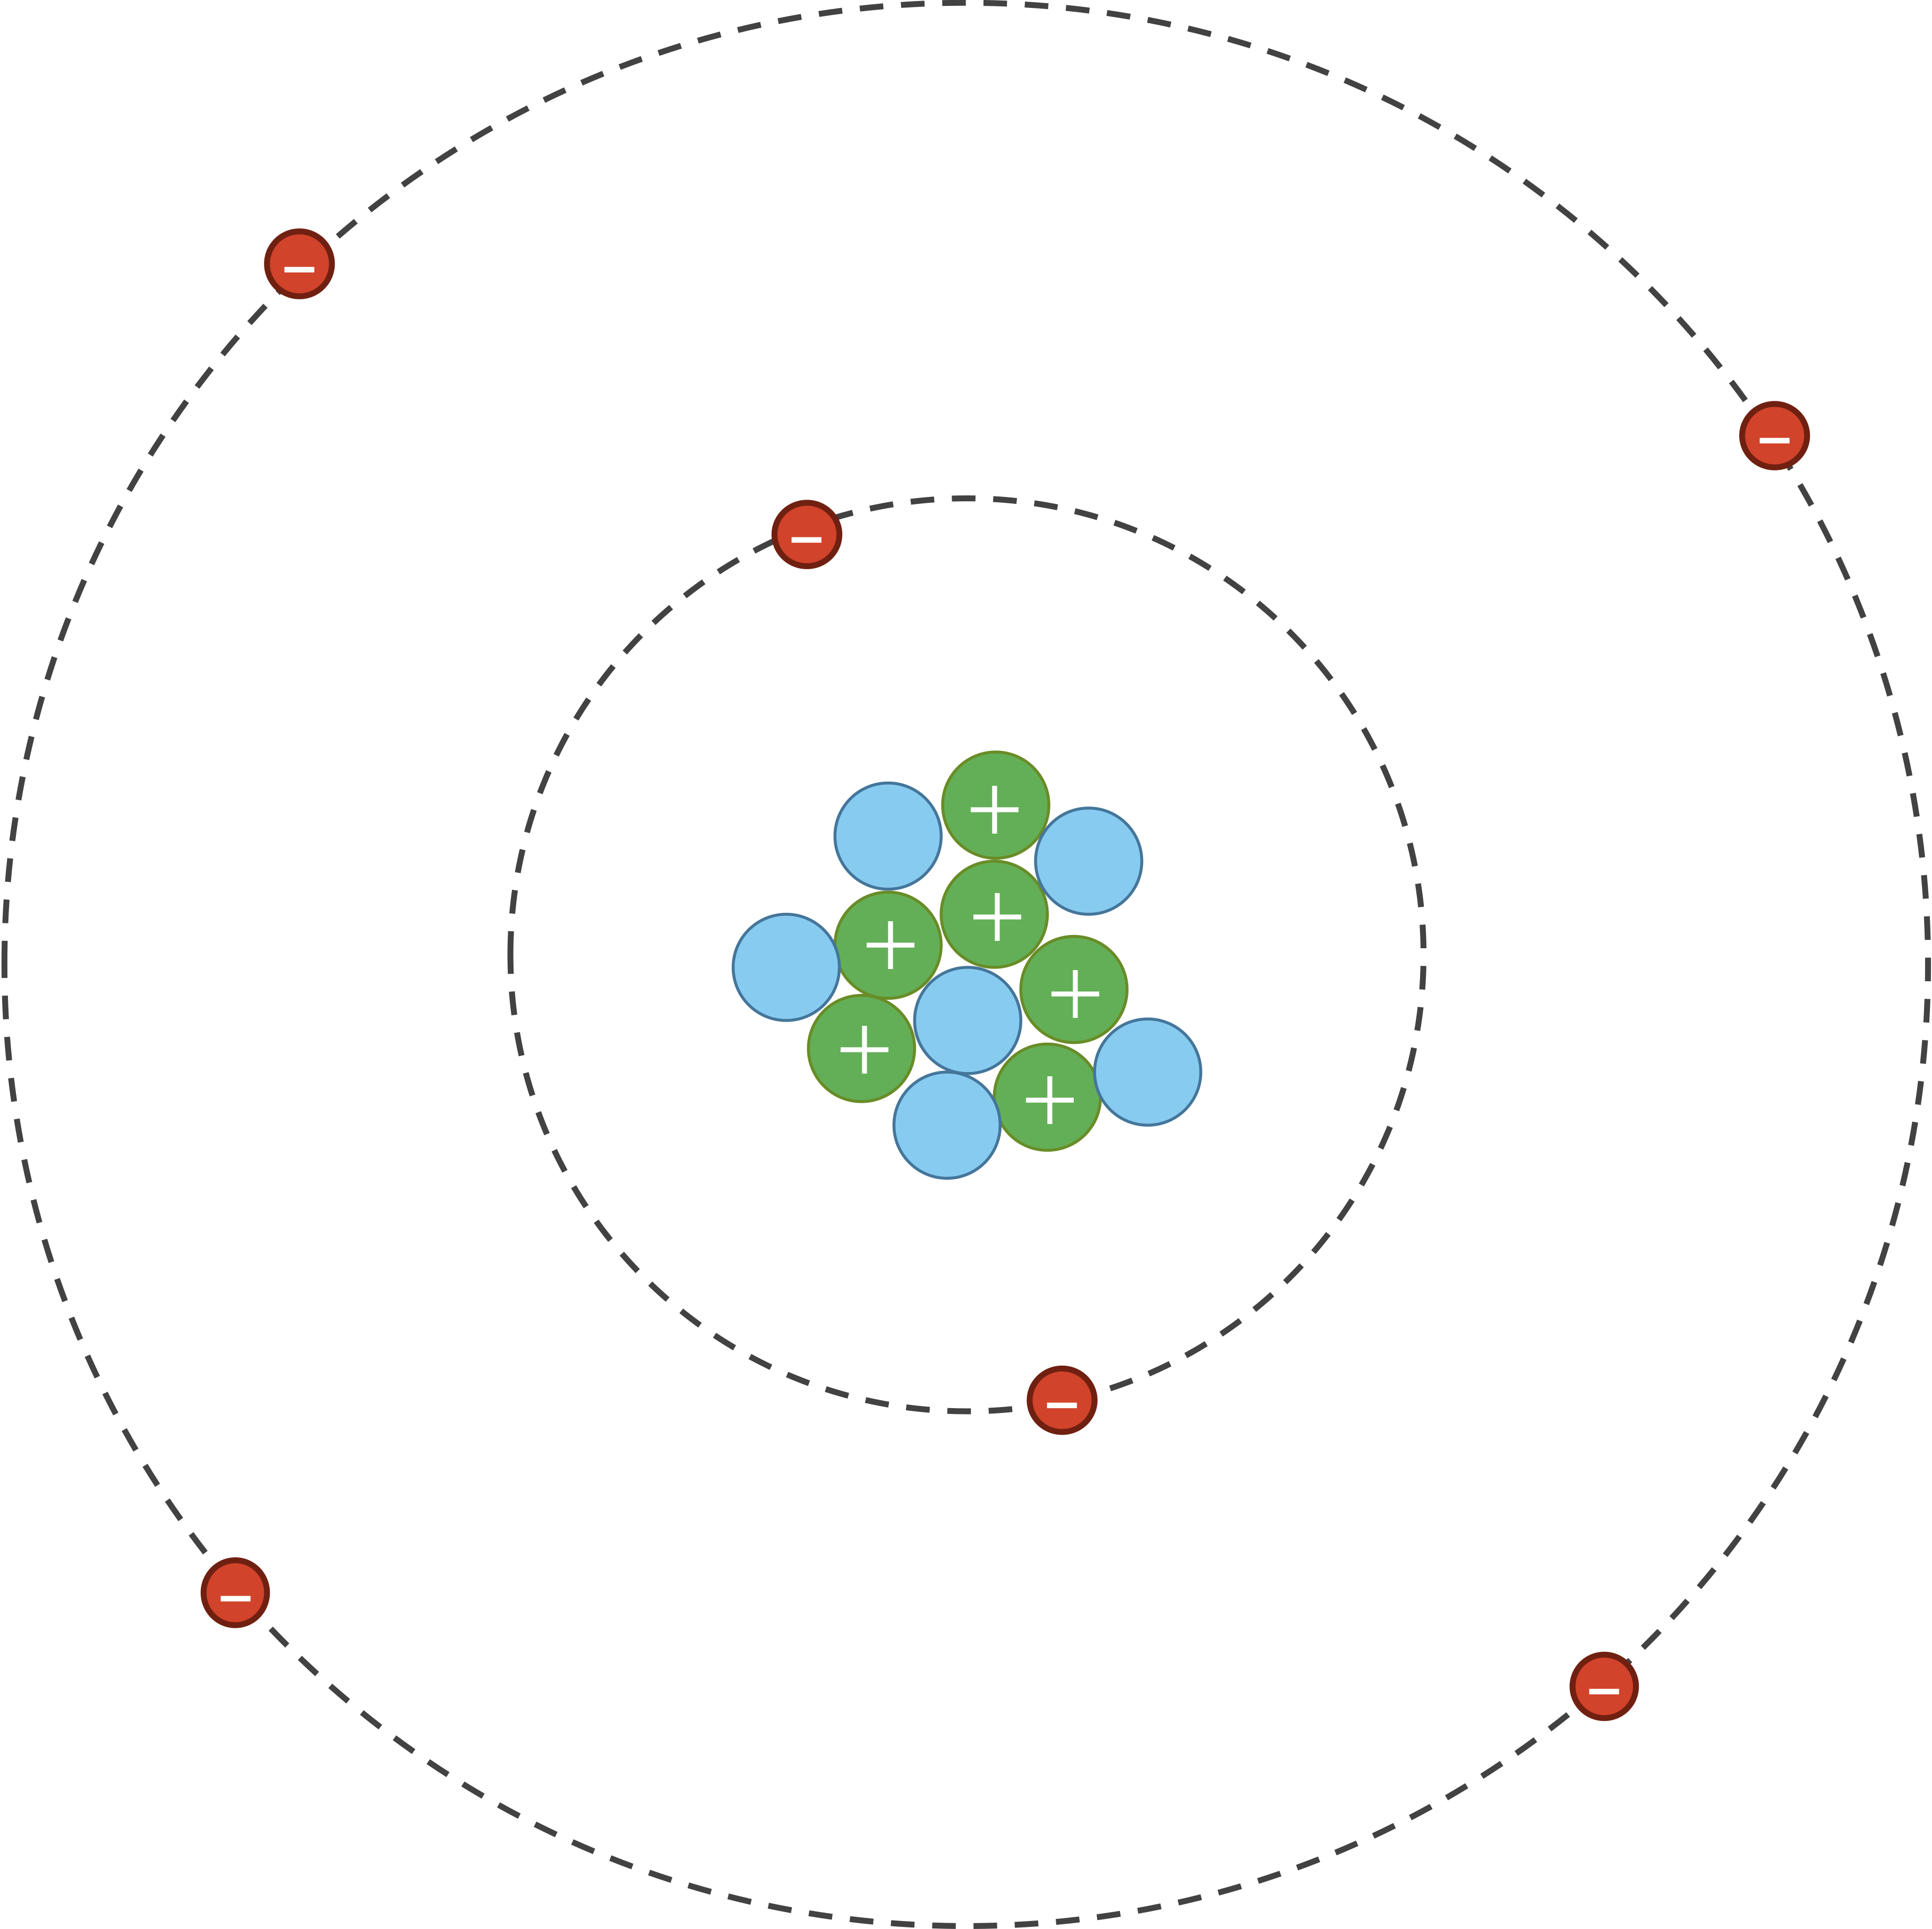
\includegraphics[width = 0.4\textwidth]{../images/van_der_waals_normal.png}
%	\caption{A carbon-12 atom showing six positively charged protons (green), six neutrally charged neutrons (blue), and six negatively charged electrons (red). Under typical circumstances, the electrons will most likely be distributed uniformly around the nucleus.}
%	\label{fig:van_der_waals_normal}
%\end{figure}

\begin{figure}[h]
	\centering
	\mySfFamily
	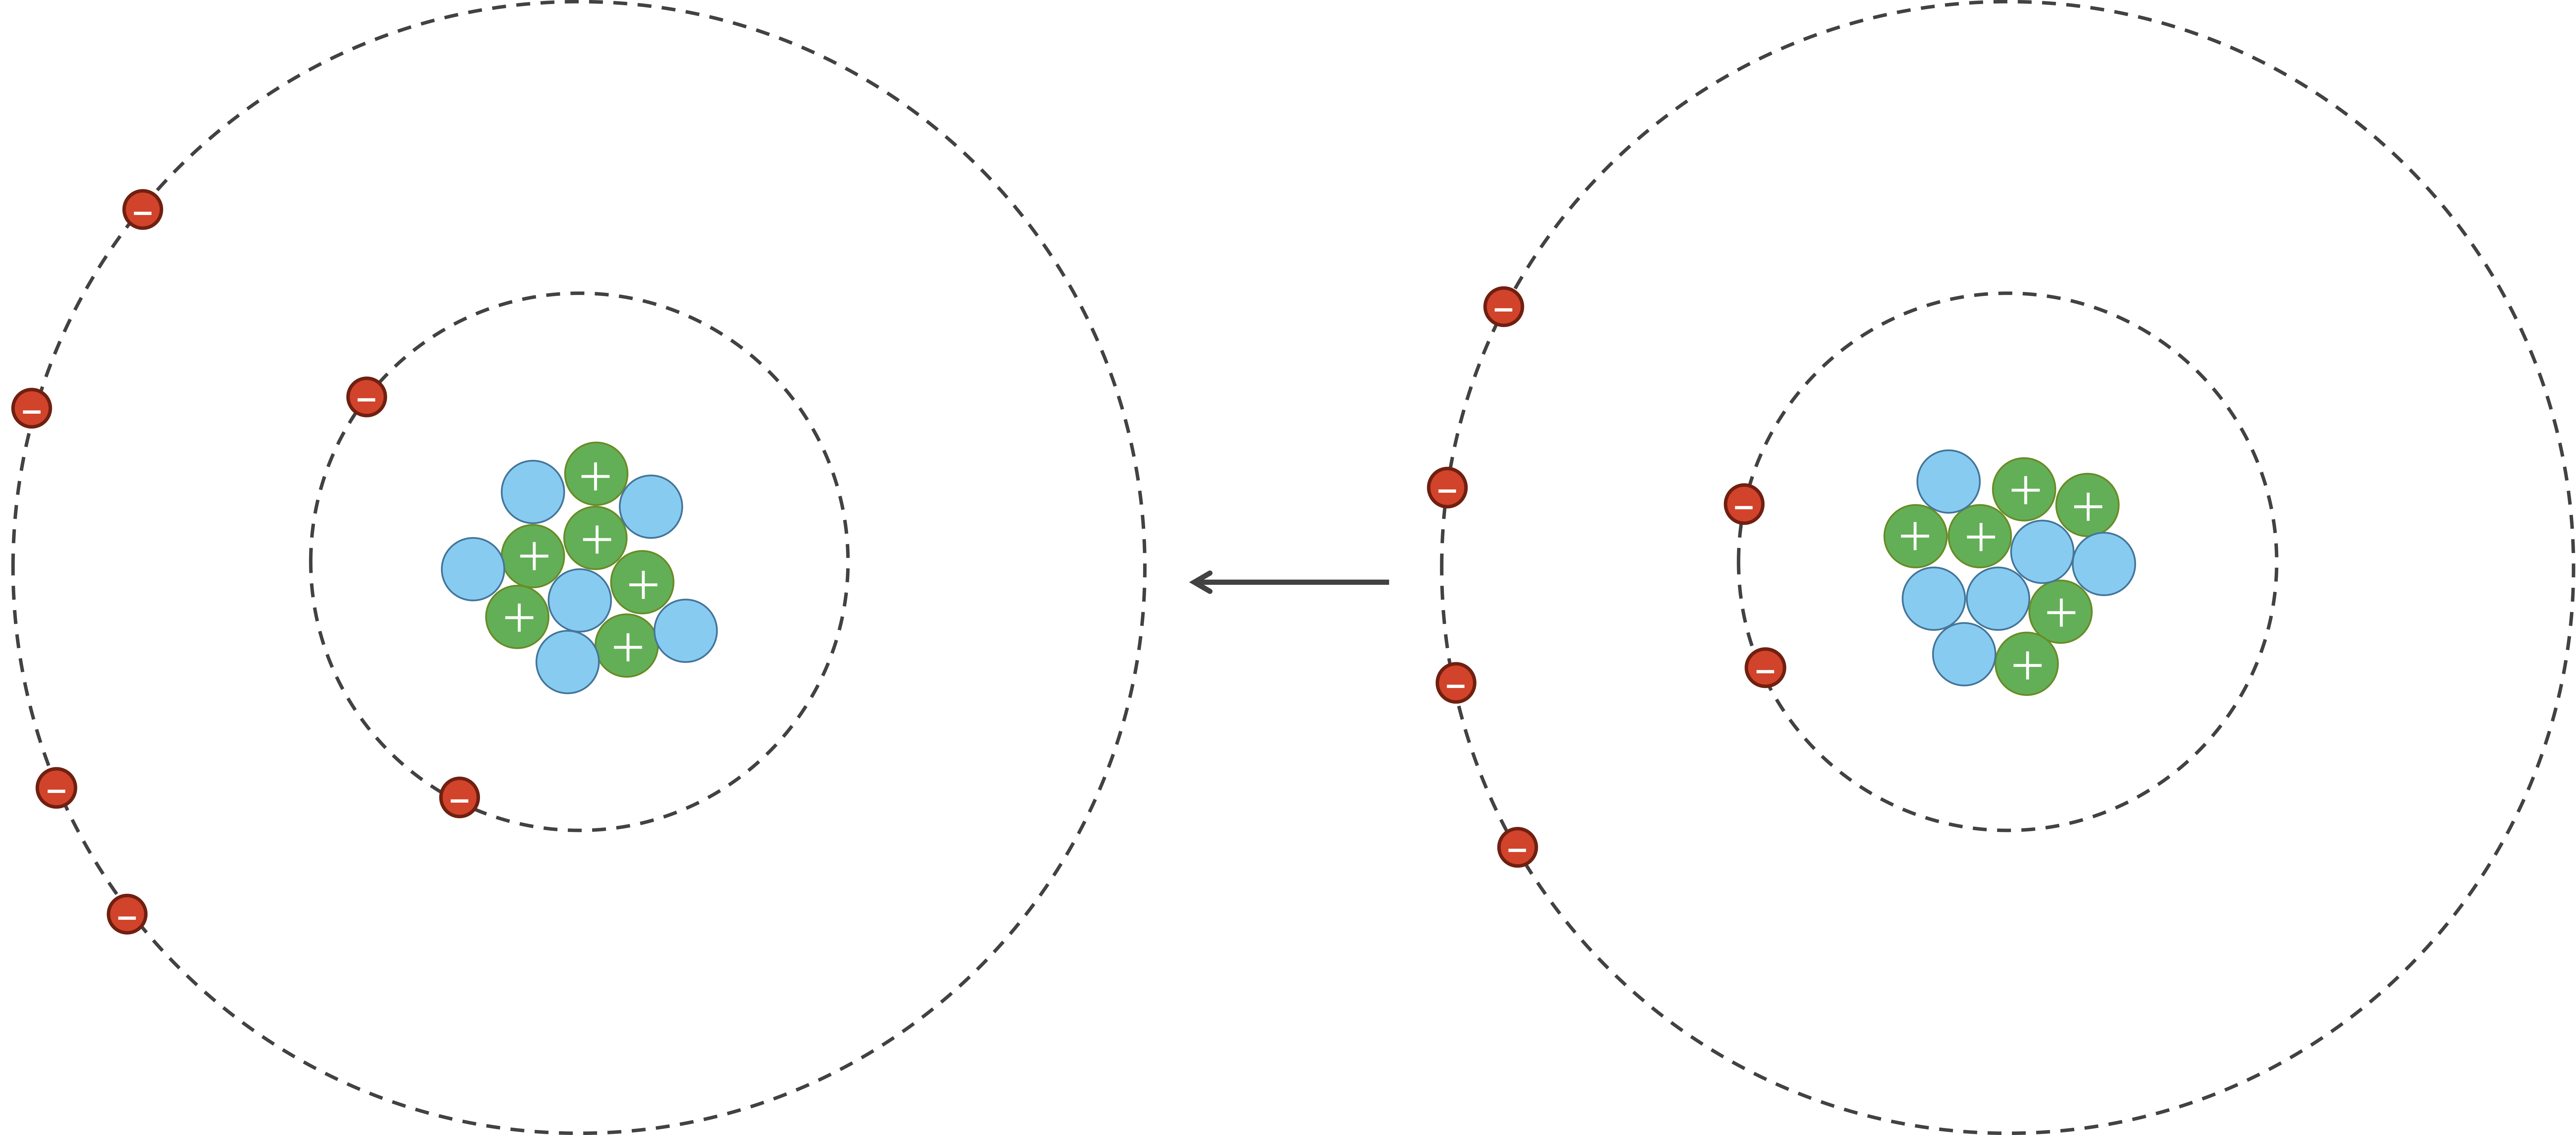
\includegraphics[width = 0.85\textwidth]{../images/van_der_waals.png}
	\caption{Due to random chance, the electrons in the atom on the left have clustered on the left side of the atom, creating a net negative charge on this side of the atom, and therefore a net positive charge on the right side of the atom. This polarity induces a dipole in the atom on the right, whose electrons are attracted because of van der Waals forces.}
	\label{fig:van_der_waals}
\end{figure}

As the protein folds, it seeks a conformation of \textit{lowest} total potential energy based on the combination of all these forces. For an analogy, imagine a ball on a slope (\autoref{fig:EnergyCartoon}). The ball will tend to move down the slope unless it is pushed uphill by some outside force, making it unlikely that the ball will wind up at the top of a hill. We will keep this analogy in mind as we return to the problem of protein structure prediction.\\

\begin{figure}[h]
	\centering
	\mySfFamily
	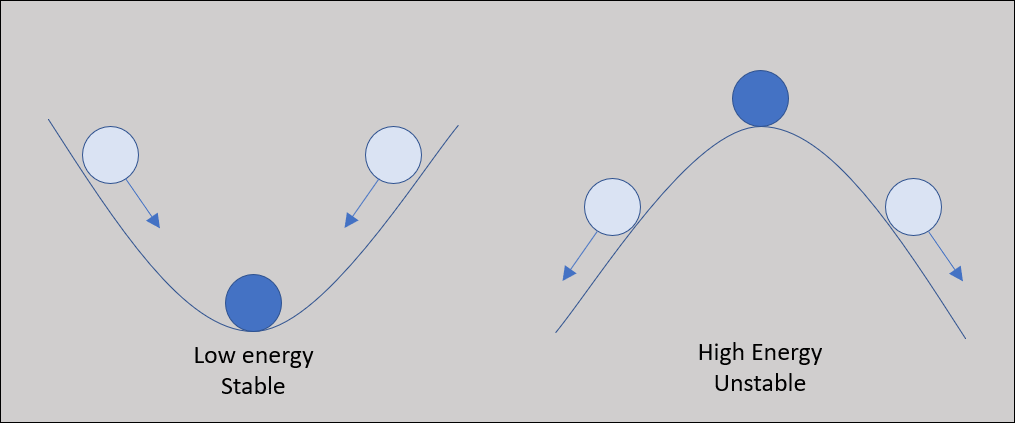
\includegraphics[width = 0.85\textwidth]{../images/EnergyCartoon.png}
	\caption{A ball on a slope offers a classic analogy for a protein folding into the lowest energy structure. As the ball is more likely to move down into a valley, a protein is more likely to fold into a more stable, low-energy conformation.}
	\label{fig:EnergyCartoon}
\end{figure}

\FloatBarrier
\phantomsection

\section{\textit{Ab initio} Protein Structure Prediction}
\label{sec:ab_initio}

\phantomsection
\subsection{Modeling \textit{ab initio} structure prediction as an exploration problem}

Predicting a protein’s structure using only its amino acid sequence is called \textdef{\textit{ab initio} structure prediction}{ab initio structure prediction}{the prediction of a protein's structure using only its amino acid sequence} (\textit{ab initio} means “from the beginning” in Latin). Although many different algorithms have been developed for \textit{ab initio} protein structure over the years, these algorithms all find themselves solving a similar problem.

Biochemical research has contributed to the development of scoring functions called \textdef{force fields}{force field}{an approach that estimates forces between atoms within or between molecules} that use the physicochemical properties of amino acids introduced in the previous section to compute the potential energy of a candidate protein shape. For a given choice of force field, we can think of \textit{ab initio} structure prediction as solving the following problem: given a primary structure of a polypeptide, find its tertiary structure having minimum energy. This problem exemplifies an \textdef{optimization problem}{optimization problem}{a problem in which we are seeking an object maximizing or minimizing some function subject to constraints}, in which we are seeking an object maximizing or minimizing some function subject to constraints.

This formulation of protein structure prediction may not strike you as similar to anything that we have done before in this course. However, consider once more a bacterium exploring an environment for food. Every point in the bacterium's ``search space'' is characterized by a concentration of attractant, and the bacterium's goal is to reach the point of maximum attractant concentration.

In the case of structure prediction, our search space is the collection of all possible conformations of a given protein, and each point in this search space is characterized by the energy of the conformation at the point. Just as we imagined a ball rolling down a hill to find lower energy in \autoref{fig:EnergyCartoon}, we can now imagine exploring the search space of all conformations of a polypeptide to find the conformation having lowest energy. The general problem of exploring a search space to find a point minimizing some function is illustrated in \autoref{fig:energy_landscape}, in which the height of each point represents the function value, and our goal is to find the lowest point in the space.\\

\begin{figure}[h]
	\centering
	\mySfFamily
	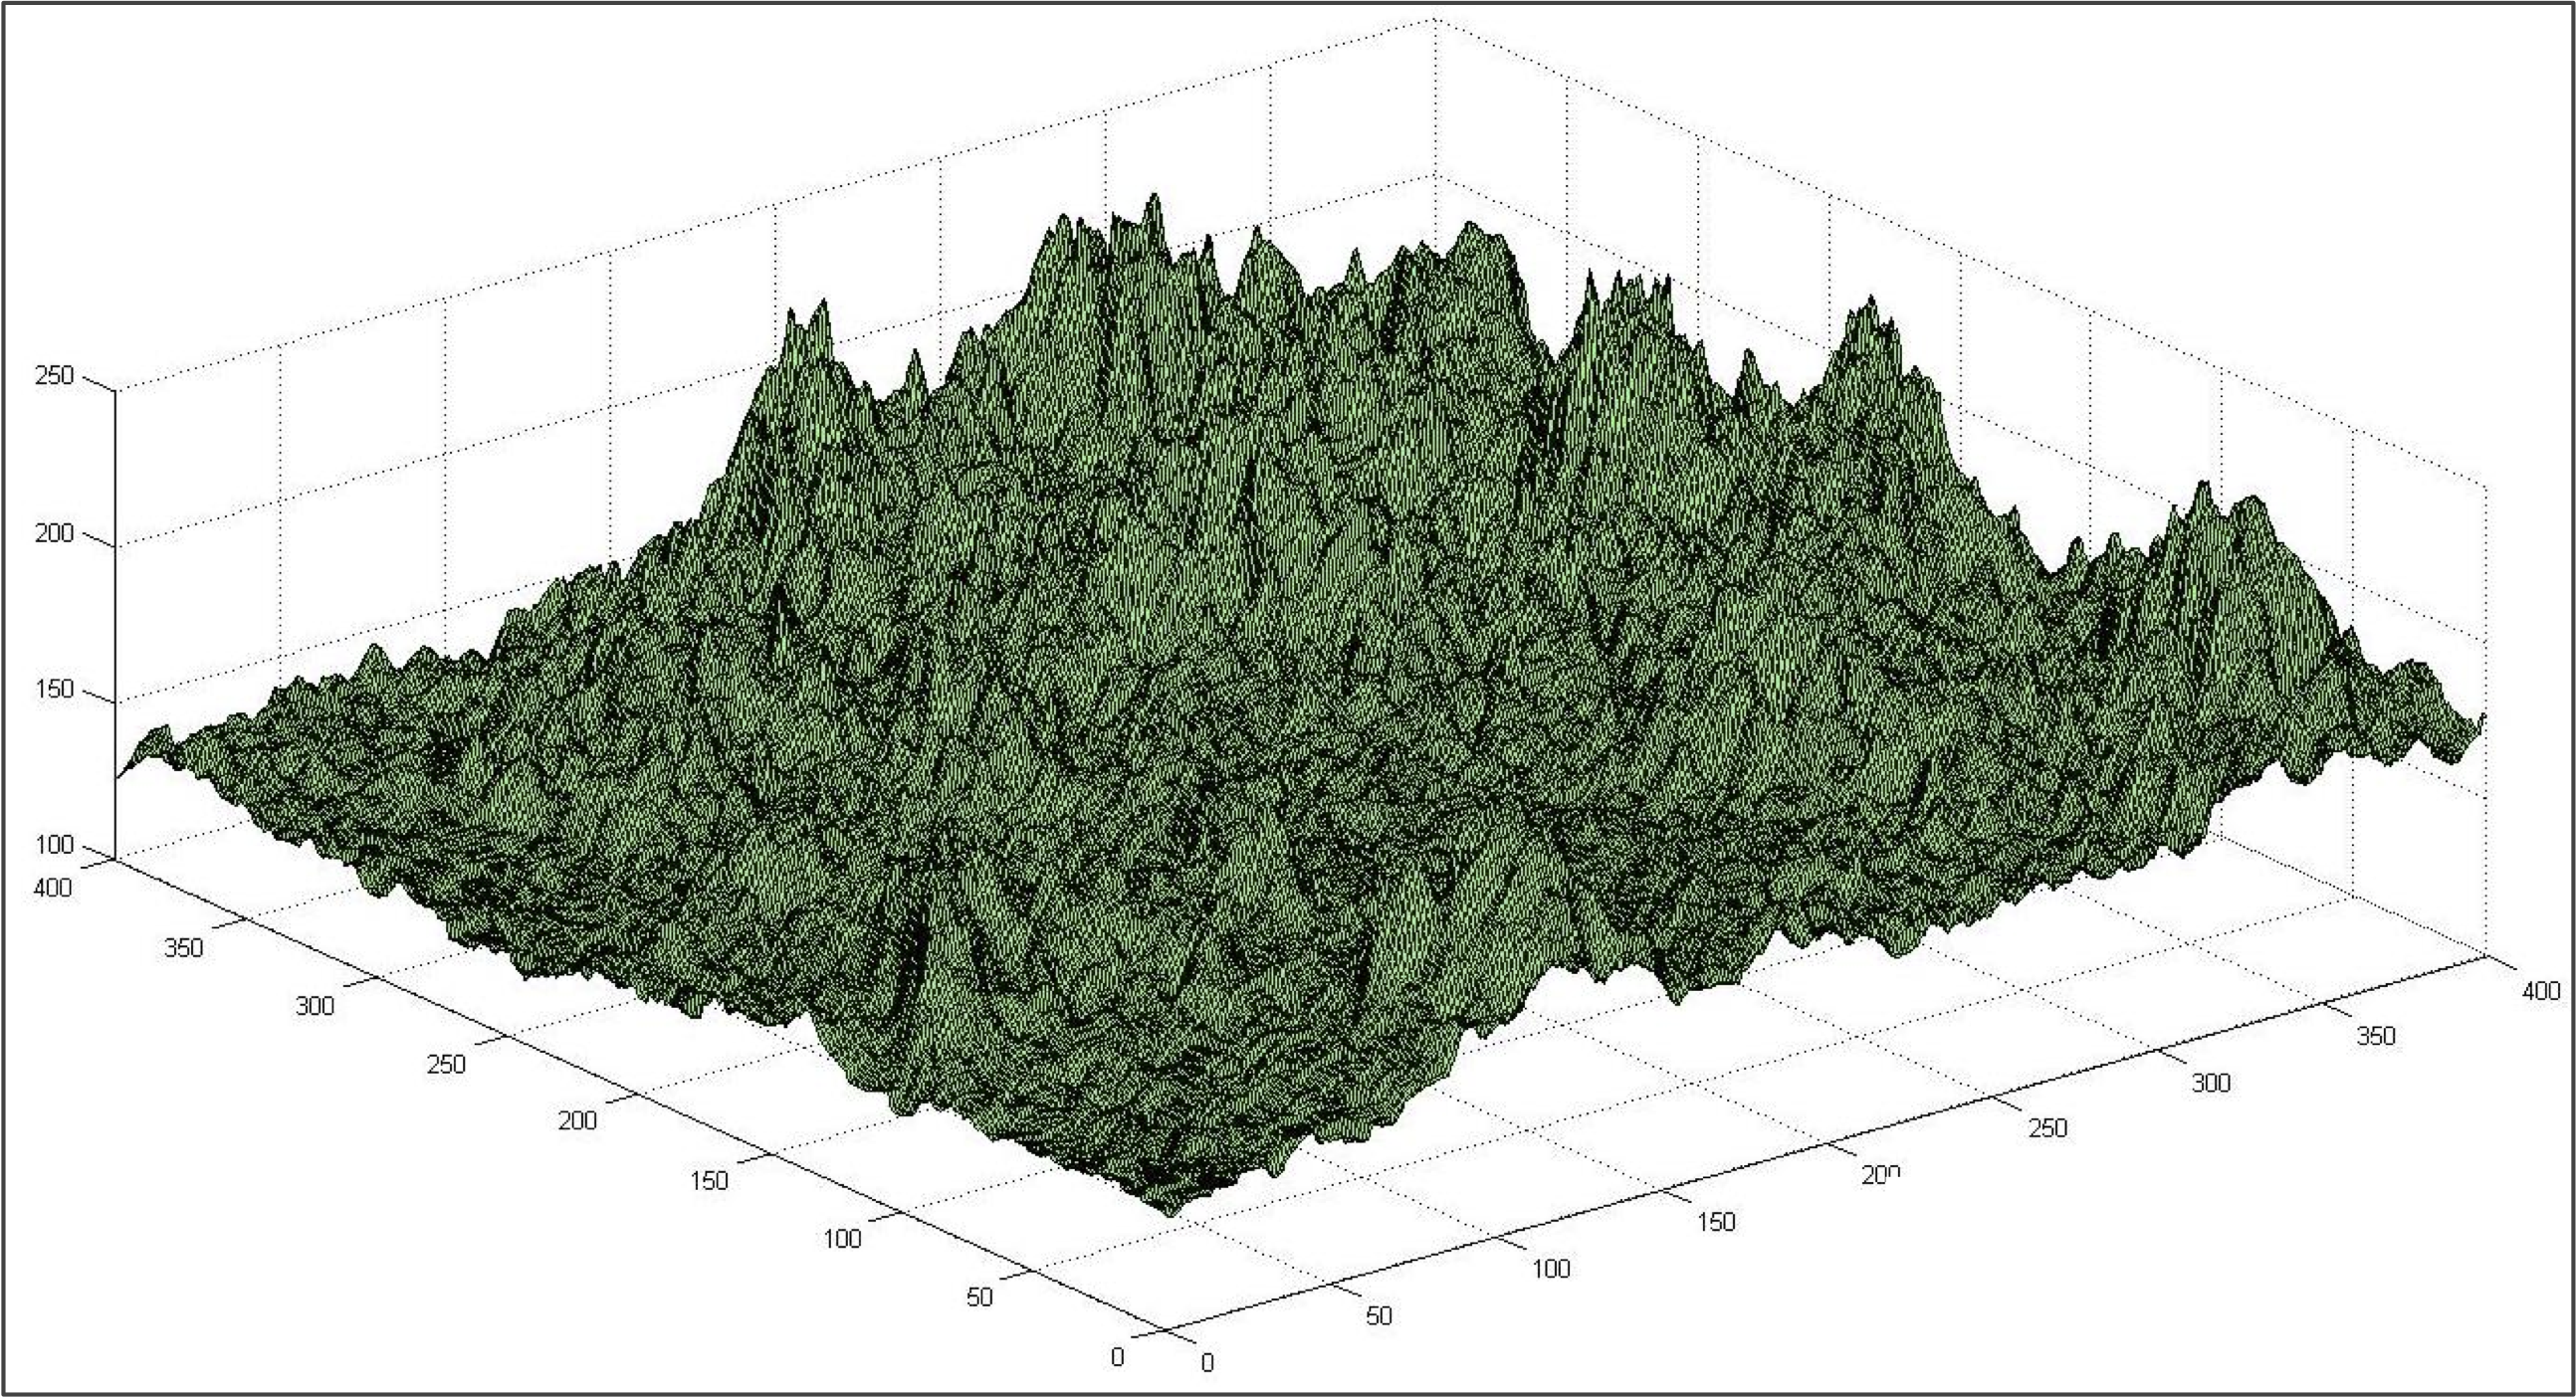
\includegraphics[width = 0.7\textwidth]{../images/energy_landscape.png}
	\caption{Optimization problems can be thought of as exploring a search space, visualized as a landscape, in which the height of a point is the value of the function that we wish to optimize. Finding the highest or lowest point in this landscape corresponds to maximizing or minimizing the function over the search space.}
	\label{fig:energy_landscape}
\end{figure}

\FloatBarrier
\phantomsection
\subsection{A local search algorithm for \textit{ab initio} structure prediction}

Now that we have conceptualized finding the most stable protein structure as exploring a search space, we turn to developing an algorithm to explore this space. Our idea is to use an approach similar to \textit{E. coli}'s clever exploration algorithm from \autoref{chapter:chemotaxis}: over a sequence of steps, we will consult a collection of nearby points in the space, and then move in the ``direction'' in which the energy function decreases by the most. This approach belongs to a broad category of optimization algorithms called \textdef{local search algorithms}{local search algorithm}{an algorithm for an optimization problem that explores a search space by making subsequent small modifications to an object of interest}.

Adapting this exploration algorithm to protein structure prediction requires us to develop a notion of what it means to consider the points ``nearby'' a given conformation in a protein search space. Many \textit{ab initio} algorithms will start at an arbitrary initial conformation and then make a variety of minor modifications to that structure (i.e., nearby points in the space), updating the current conformation to the modification that produces the greatest decrease in free energy. These algorithms then iterate the process of changing the protein structure to have greatest decrease in potential energy. They terminate the search after reaching a structure for which no changes to the structure reduce the free energy.

Yet returning to the chemotaxis analogy, imagine what happens if we were to place many small sugar cubes and one large sugar cube into the bacterium's environment. The bacterium will sense the gradient not of the large sugar cube but of its \textit{nearest} attractant. Because the smaller food sources outnumber the larger food source, the bacterium will likely not reach the point of greatest attractant concentration. In bacterial exploration, this is a feature, not a bug; if the bacterium exhausts one food source, then it will just move to another. But in protein structure prediction, we should be wary of returning a protein structure that does not have minimum free energy but does have the property that no ``nearby'' structures have lower energy.

In general, an object in a search space that has a smaller value of the optimization function than neighboring points is called a \textdef{local minimum}{local minimum}{a candidate solution to an optimization problem that does not solve the problem but that has a smaller value of the optimization function than neighboring structures}. Returning to our landscape analogy from \autoref{fig:energy_landscape}, our search space may have many valleys, but in an optimization problem we would like the one that is as low as possible over the entire space, called a \textdefnogloss{global minimum}.\\

\begin{qbox}[%
	How could we improve our local search approach for structure prediction to avoid winding up in a local minimum?
	]\end{qbox}

Researchers applying local search algorithms have devised a number of ways to avoid local minima, and two are so fundamental as to be worth mentioning here. First, because the initial conformation has a huge influence on the final conformation, we could run the algorithm multiple times with different starting conformations. This is analogous to allowing multiple bacteria to explore their environment at different starting points. Second, every time we reach a local minimum, we could allow ourselves to change the structure with some probability, thus giving our local search algorithm the chance to ``bounce'' out of the local minimum. Once again, randomized algorithms help us solve problems!

\FloatBarrier
\phantomsection
\subsection{Applying an \textit{ab initio} algorithm to a protein sequence}

To run an \textit{ab initio} structure prediction algorithm on a real protein, we will use a software resource called \href{https://zhanglab.ccmb.med.umich.edu/QUARK/}{QUARK}, which is built upon the ideas discussed in the previous section, with some added features. For example, its algorithm applies a combination of \textit{multiple} scoring functions to look for the lowest energy conformation across all of these functions.

Levinthal's paradox means that the search space of all possible structures for a protein is so large that accurately predicting large protein structures with \textit{ab initio} modeling remains very difficult. As such, QUARK limits us to proteins with at most 200 amino acids, and so we will run it only on human hemoglobin subunit alpha.\tutorial[coronavirus/tutorial_ab_initio]

\autoref{fig:ab_initio_results} shows the top five predicted human hemoglobin subunit alpha structures returned by QUARK as well as the protein's experimentally verified structure, and an average of these six structures. It takes a keen eye to see any differences between all these structures. We conclude that although \textit{ab initio} prediction is slow, it is nevertheless accurate. Yet we also wonder if we can speed up our structure prediction algorithms so that they will scale to a larger protein like the SARS-CoV-2 spike protein.\\

\begin{figure}[h]
	\centering
	\mySfFamily
	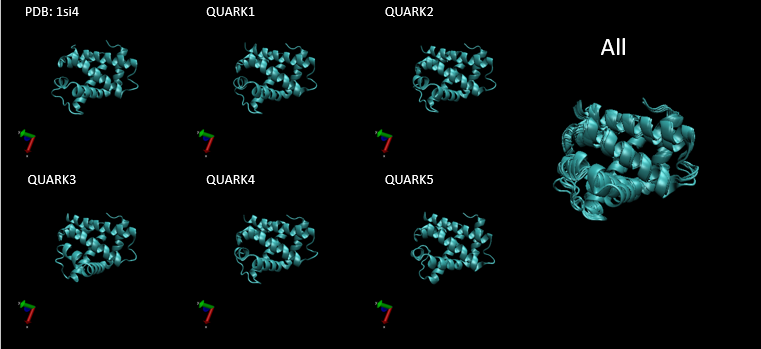
\includegraphics[width = 0.85\textwidth]{../images/ab_initio_results.png}
	\caption{The experimentally verified protein structure of human hemoglobin subunit alpha (top left) along with five models of this protein produced by QUARK from the protein's primary sequence. We can see how close all five models are to the experimentally verified structure, as shown in the superimposition of all six structures at right.}
	\label{fig:ab_initio_results}
\end{figure}

\begin{qbox}[%
What known protein structure(s) would you first want to consult when studying the SARS-CoV-2 spike protein?
]\end{qbox}

\FloatBarrier
\phantomsection

\section{Homology Modeling}
\label{sec:homology}
\phantomsection
\subsection{Homology modeling finds a similar protein structure}

Although \textit{ab initio} structure prediction can be challenging, we also mentioned that researchers have entered over 160,000 experimentally verified structure entries into the PDB. With every new structure that we identify, we gain a little more insight into nature's magic protein folding algorithm. In \textdef{homology modeling}{homology modeling}{an approach for protein structure prediction, also known as comparative modeling, in which we use the information contained in known structures to help us predict the structure of a protein with unknown structure} (also called \textdefnogloss{comparative modeling}), we use the information contained in known structures to help us predict the structure of a protein with unknown structure.

The structure of the SARS-CoV spike protein was determined in 2003. Assuming that the two proteins have similar structure, we will use SARS-CoV spike protein's known structure as a guide to help us predict the structure of the SARS-CoV-2 spike protein. In other words, if the search space of all conformations of the SARS-CoV-2 spike protein is enormous, why not restrict it to those structures that are similar to the SARS-CoV spike protein structure?\\

\begin{qbox}[%
In the case of the SARS-CoV-2 spike protein, we already know that we want to use the SARS-CoV spike protein as a template. However, if we do not know which template to use before we begin, how could we find a candidate protein template?
]\end{qbox}

\phantomsection
\subsection{A similar structure reduces the size of the search space}

Once we have found a protein with potentially similar structure to our protein of interest, we need to use it to predict the structure of this protein. One way of doing so is to include a ``similarity term'' in the energy function that subtracts a structure's similarity to the template structure from the structure's total energy. That is, the more similar that a candidate structure is to the template, the more negative the contribution of this similarity term. To continue our search space analogy, the template protein ``pulls down'' the energy values of nearby structures like a gravity well.

Another way to perform homology modeling is to account for variance in similarity across different regions of the two proteins. The SARS-CoV and SARS-CoV-2 genomes are 96\% similar, but their spike proteins are only 76\% similar. In general, when we examine genomes from related species, we see \textdefnogloss{conserved regions} where the species are very similar and other \textdefnogloss{variable regions} where the species are more different than the average.

The phenomenon of conserved and variable regions also occurs within individual genes. \autoref{fig:spike_protein_similarity} shows that within a spike protein subunit, the S2 domain is 90\% similar between the two viruses, whereas the S1 domain is only 64\% similar. Furthermore, the S1 domain divides into two subunits of differing similarity.

\begin{figure}[h]
	\centering
	\mySfFamily
	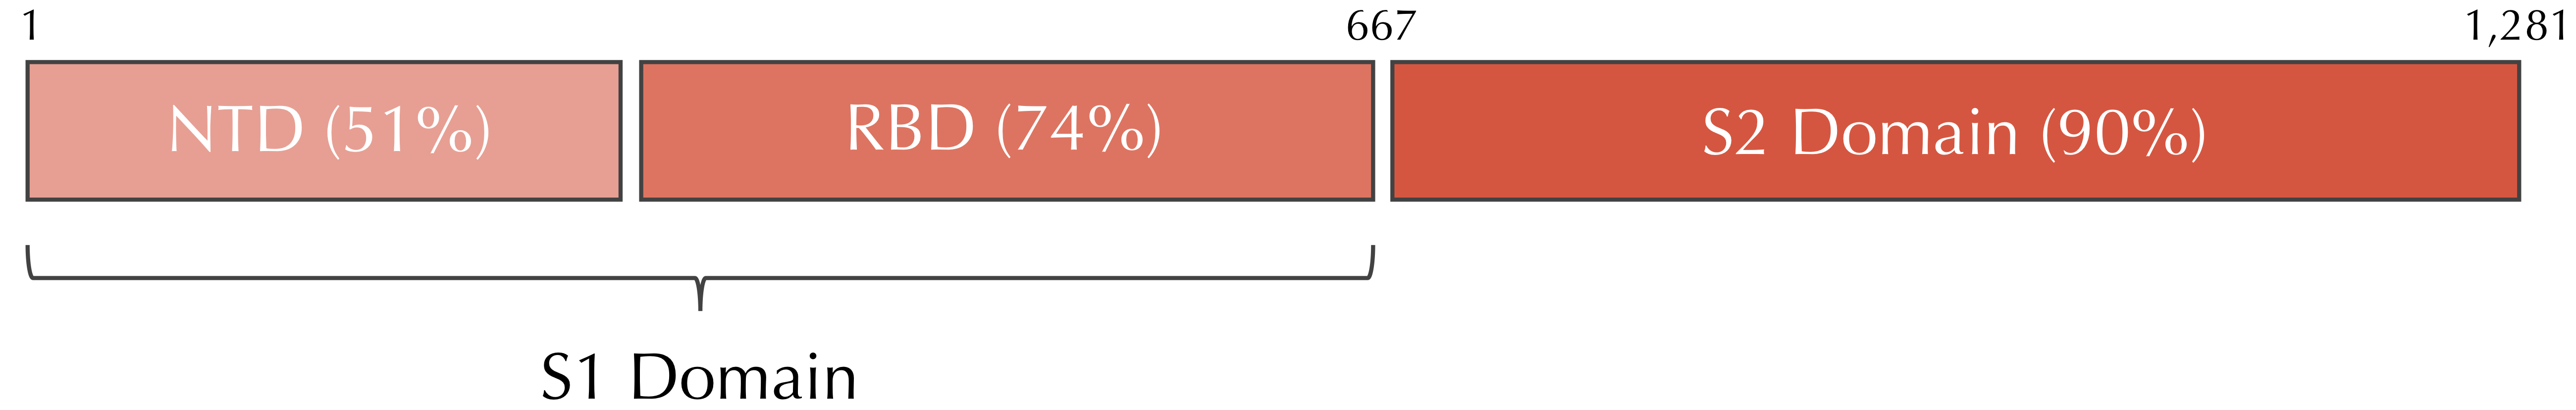
\includegraphics[width = 0.85\textwidth]{../images/spike_protein_similarity.png}\\
	\caption{Variable and conserved regions in the SARS-CoV and SARS-CoV-2 spike proteins. The S1 domain tends to be more variable, whereas the S2 domain is more conserved. In this figure, ``NTD'' stands for ``N-terminal domain'' and ``RBD'' stands for ``receptor binding domain'', two subunits of the S1 domain.}
	\label{fig:spike_protein_similarity}
\end{figure}

Some homology modeling algorithms account for variable and conserved regions by assuming that very conserved regions in the two genes correspond to essentially identical structures in the proteins. That is, the structure of our protein of interest in these regions will be the same as those of the template protein. We can then use a \textdefnogloss{fragment library}, a catalog of known substructures from many proteins, to fill in the structure of non-conserved regions based on structures of fragments whose sequence is similar to these regions. This approach is called \textdef{fragment assembly}{fragment assembly}{the process of using a library of known substructures from many proteins to fill in the structure of non-conserved regions when predicting a protein's structure}.

We will model the SARS-CoV-2 spike protein using homology modeling software from three publicly available fragment assembly servers (SWISS-MODEL, Robetta, and GalaxyWEB). If the results are similar, then we have faith in the \textit{robustness} of our predictions when using different approaches. Furthermore, comparing the results of multiple different approaches may give us more insights into structure prediction. If you are not interested in following this tutorial, links to the results can be found in \autoref{fig:homology_modeling_results_table}.\tutorial[coronavirus/tutorial_homology]\\

\begin{figure}[h]
	\centering
	\tabcolsep = 1 em
	\mySfFamily
	\begin{tabular}{c c}
		\textbf{Structure Prediction Server} & \textbf{Results} \\
		SWISS-MODEL (spike protein) & \url{https://bit.ly/3gIR1RC} \\
		Robetta (Single-Chain spike protein) & \url{https://bit.ly/34XMmsd} \\
		GalaxyWEB & \url{https://bit.ly/34WsKES} \\
	\end{tabular}
	\caption{A table containing links to the prediction results of three homology modeling software resources. SWISS-MODEL was used to predict the structure of the SARS-CoV-2 spike protein. Robetta was used to predict the structure of a single chain of the spike protein. GalaxyWEB was used to predict the structure of the spike protein's receptor binding domain (RBD).}
	\label{fig:homology_modeling_results_table}
\end{figure}

\FloatBarrier

\phantomsection
\subsection{Experiments determine the structure of the SARS-CoV-2 spike protein}

On February 25, 2020, two months after the publication of the SARS-CoV-2 genome, researchers from the Seattle Structural Genomics Center for Infectious Disease uploaded to the PDB the result of a cryo-EM experiment for the SARS-CoV-2 spike protein, which became entry \href{http://www.rcsb.org/structure/6VXX}{6vxx}.\\

\begin{note}[%
	If you would like to explore the structure of the SARS-CoV-2 spike protein, check out the 3-D protein viewer at \url{https://www.rcsb.org/3d-view/6VXX}.
	]\end{note}
	
We now turn to the problem of comparing our homology modeling results of the SARS-CoV-2 spike protein against the experimentally verified structure of SARS-CoV-2. How to compare two protein structures is a simple question, but it has a complicated answer, to which we will devote an entire section.\\

\FloatBarrier
\phantomsection

\section{Protein Structure Comparison}
\label{sec:accuracy}

\phantomsection
\subsection{Comparing two shapes with the Kabsch algorithm}

Comparing two protein structures is intrinsically similar to comparing two shapes, such as those in \autoref{fig:two_shapes}.\\

\begin{qbox}[%
	How similar are the two shapes in \autoref{fig:two_shapes}?
]\end{qbox}

\begin{figure}[h]
	\centering
	\mySfFamily
	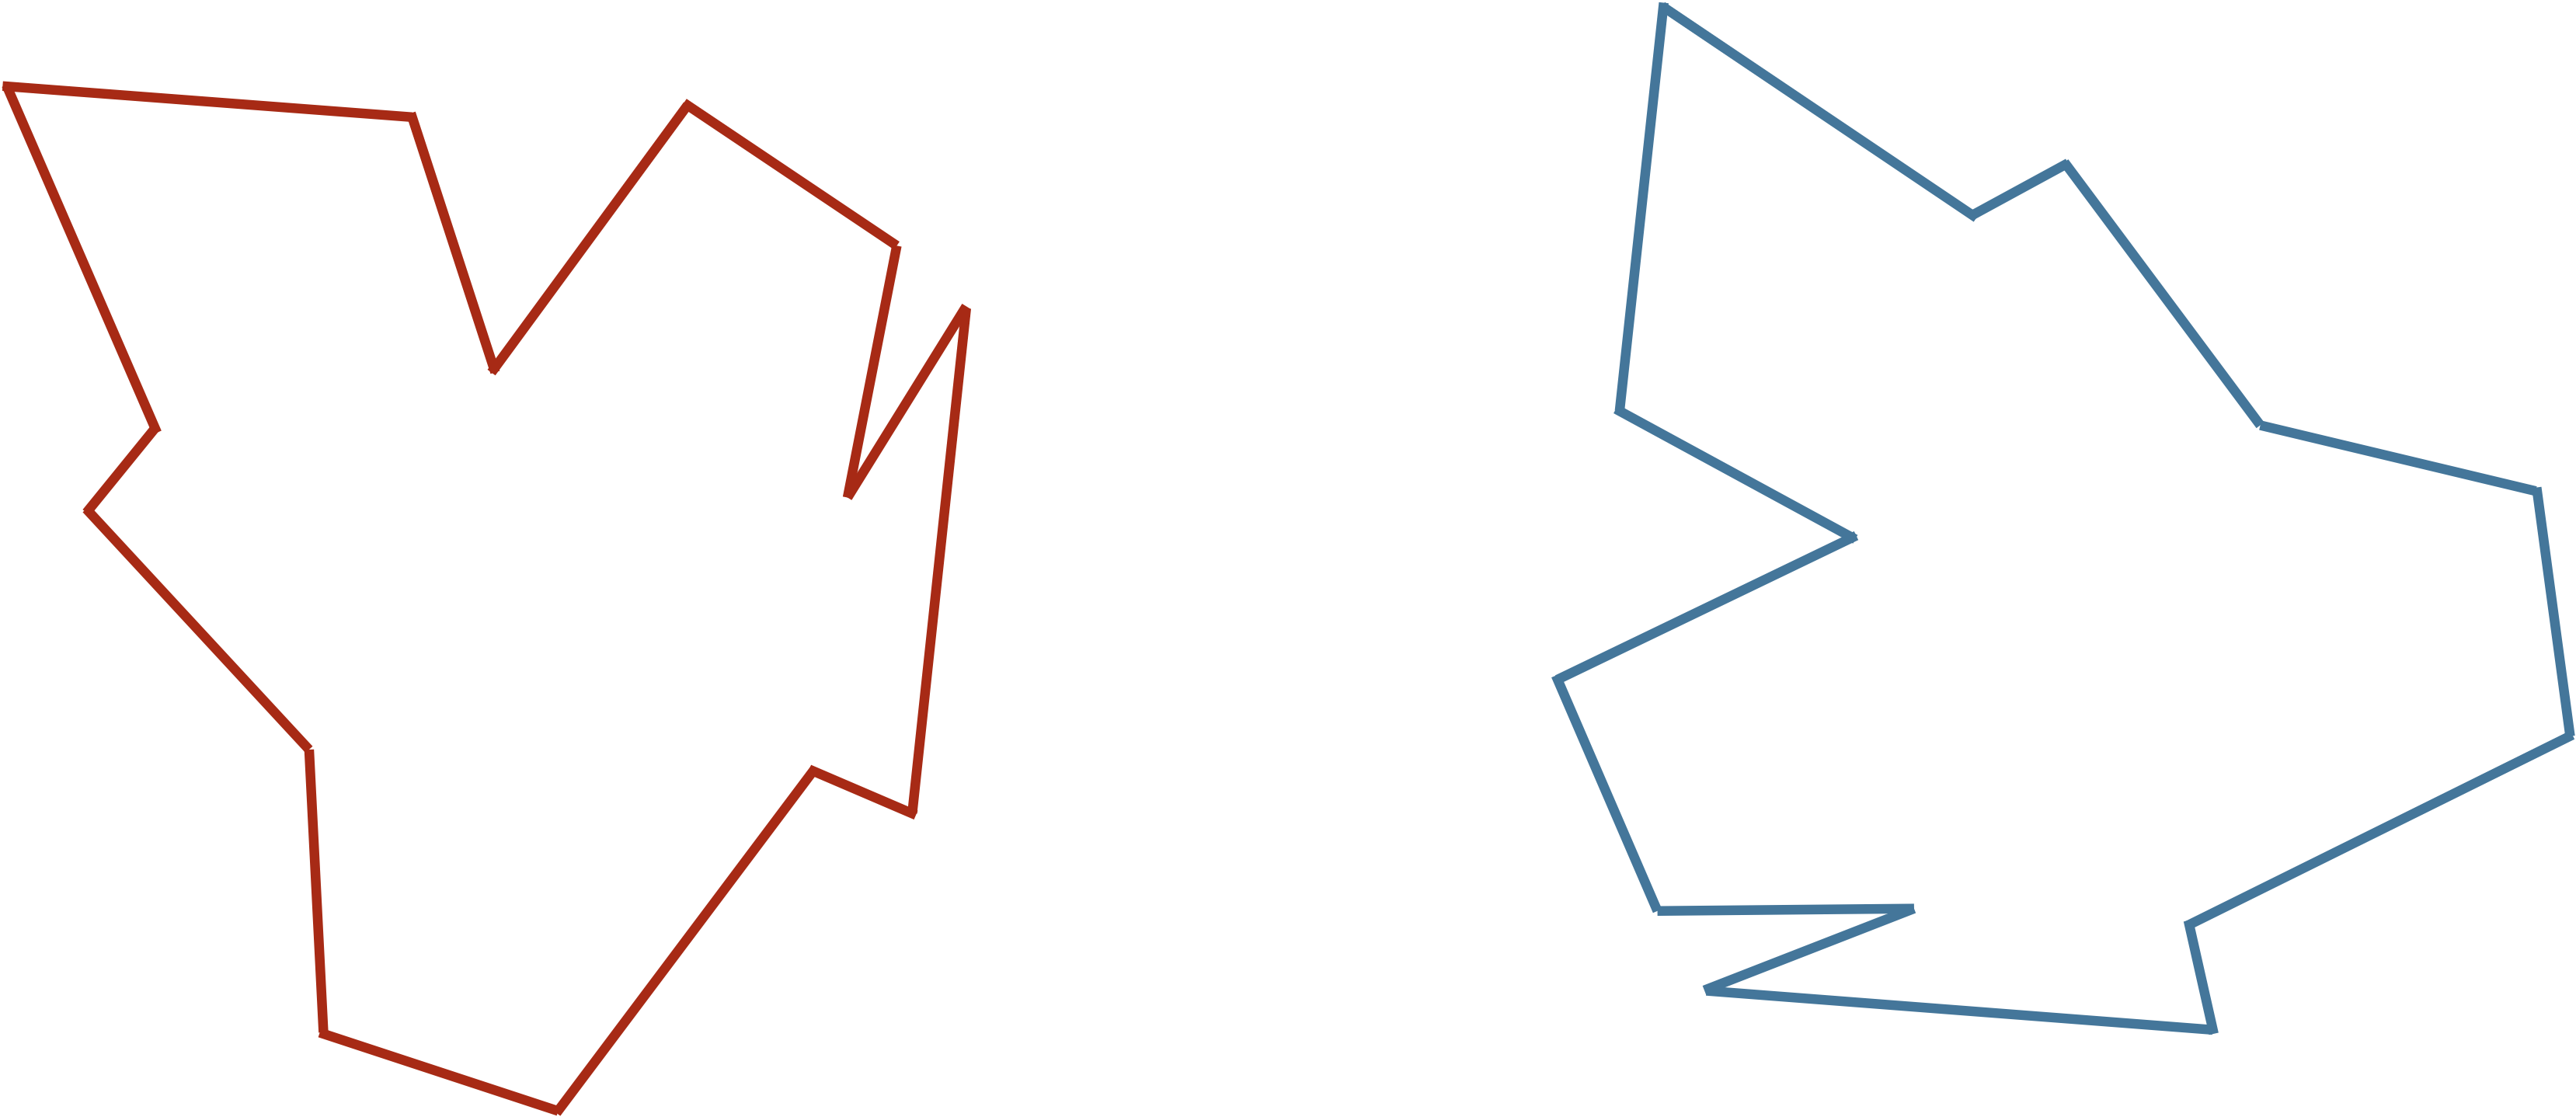
\includegraphics[width = 0.7\textwidth]{../images/two_shapes.png}
	\caption{Two example shapes.}
	\label{fig:two_shapes}
\end{figure}

If you think you have a good handle on comparing the two shapes in \autoref{fig:two_shapes}, then it is because humans have very highly evolved eyes and brains. As we will see in \autoref{chapter:white_blood_cells}, training a computer to detect and differentiate objects is more difficult than you think!

We would like to develop a distance function $d(S, T)$ quantifying how different two shapes \textit{S} and \textit{T} are. If \textit{S} and \textit{T} are the same, then $d(S, T)$ should be equal to zero; the more different \textit{S} and \textit{T} become, the larger \textit{d} should become.

You may have noticed that the two shapes in \autoref{fig:two_shapes} are, in fact, identical. To demonstrate that this is true, we can first move the red shape to superimpose it over the blue shape, then flip the red shape, and finally rotate it so that its boundary coincides with the blue shape (\autoref{fig:shape_transformation}). In general, if a shape \textit{S} can be translated, flipped, and/or rotated to produce shape \textit{T}, then \textit{S} and \textit{T} are the same shape, and so $d(S, T)$ should be equal to zero. The question is what $d(S, T)$ should be if \textit{S} and \textit{T} are not the same shape.

\begin{figure}[p]
	\centering
	\tabcolsep = 1em
	\mySfFamily
	\begin{tabular}{c}
		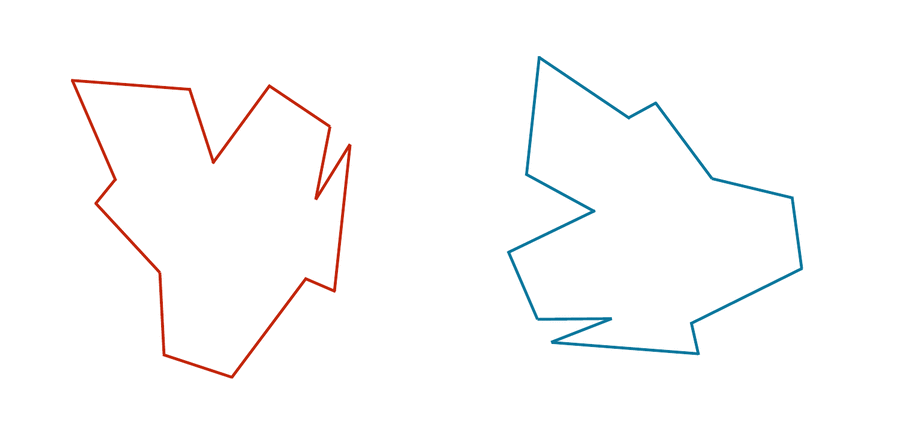
\includegraphics[width = 0.6\textwidth]{../images/shape_transformation1.png}\\[2ex]
		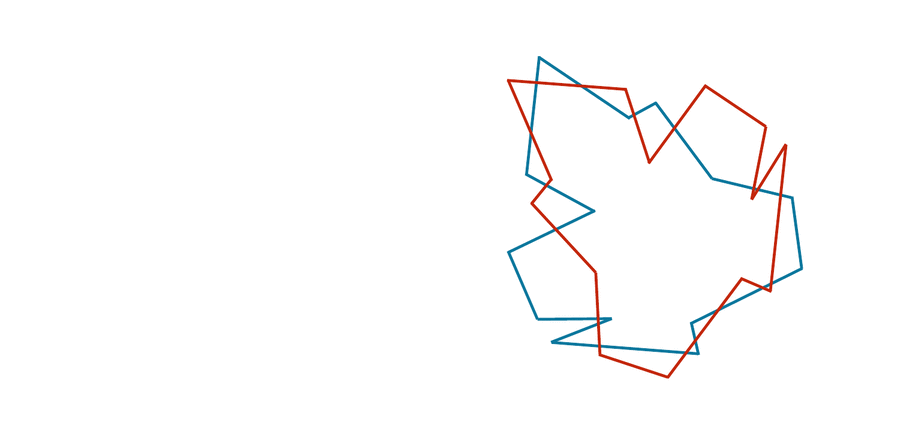
\includegraphics[width = 0.25\textwidth]{../images/shape_transformation2.png} \\[2ex]
		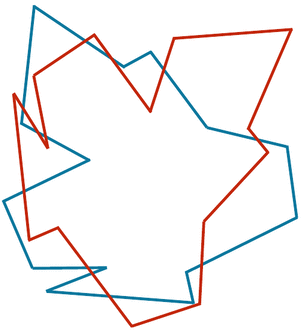
\includegraphics[width = 0.25\textwidth]{../images/shape_transformation3.png}\\[2ex]
		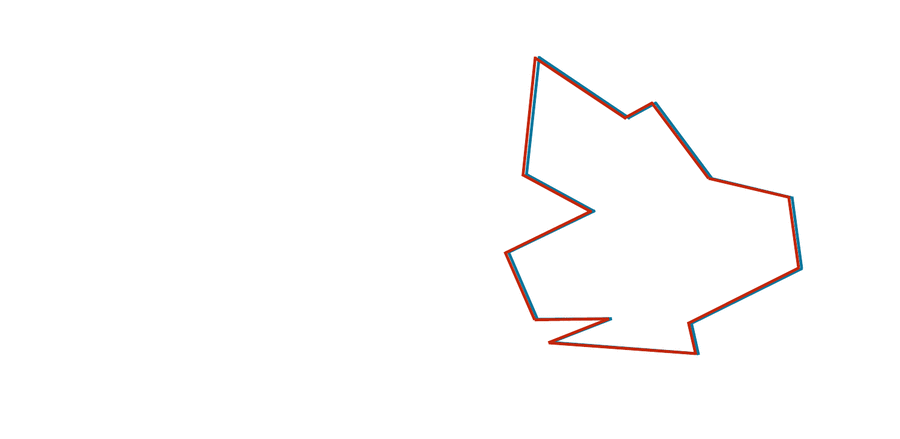
\includegraphics[width = 0.25\textwidth]{../images/shape_transformation4.png} \\
	\end{tabular}
	\caption{(First panel) The two example shapes from \autoref{fig:two_shapes}. (Second panel) aligning the two shapes. (Third panel) Flipping the red shape across its vertical axis. (Fourth panel) Rotating the red shape reveals that it is identical to the blue shape.}
	\label{fig:shape_transformation}
\end{figure}

Our idea for defining $d(S, T)$, then, is first to translate, flip, and rotate \textit{S} so that it resembles \textit{T} ``as much as possible'' to give us a fair comparison. Once we have done so, we will devise a metric to quantify the difference between the two shapes that will represent $d(S, T)$.

We first translate \textit{S} to have the same \textdef{center of mass}{center of mass}{the point corresponding to a shape whose coordinates are the averages of respective coordinates of points on the shape} as \textit{T}. The center of mass of \textit{S} is found at the point $(x_{S}, y_{S})$ such that $x_{S}$ and $y_{S}$ are the respective averages of the \textit{x}-coordinates and \textit{y}-coordinates on the boundary of \textit{S}.

The center of mass of some shapes can be determined mathematically. But for irregular shapes, we will first sample \textvar{n} points from the boundary of \textvar{S} and then estimate $x_S$ and $y_S$ as the average of all the respective \textvar{x}- and \textvar{y}-coordinates from the sampled points.

After finding the centers of mass of the two shapes \textit{S} and \textit{T} that we wish to compare, we translate \textit{S} so that it has the same center of mass as \textit{T}. We then wish to find the rotation of \textit{S}, possibly along with a flip as well, that makes the shape resemble \textit{T} as much as possible.

Imagine that we have found the desired rotation; we are now ready to define $d(S, T)$ in the following way. We sample \textit{n} points along the boundary of each shape, converting \textit{S} and \textit{T} into \textdefnogloss{vectors} $\mathbf{s} = (s_{1}, \ldots, s_{n})$ and $\mathbf{t} = (t_{1}, \ldots, t_{n})$, where $s_{i}$ is the \textit{i}-th point on the boundary of \textit{S}. The \textdef{root mean square deviation (RMSD)}{root mean square deviation (RMSD)}{the square root of the average squared distance between corresponding points in two vectors} between the two shapes is the square root of the average squared distance between corresponding points in the vectors,

\begin{center}
$\text{RMSD}(\mathbf{s}, \mathbf{t}) = \sqrt{\dfrac{1}{n} \cdot \left(d(s_1, t_1)^2 + d(s_2, t_2)^2 + \cdots + d(s_n, t_n)^2\right)}$\,.
\end{center}

\noindent In this formula, $d(s_{i}, t_{i})$ is the distance between the points $s_{i}$ and $t_{i}$.\\

\begin{note}[%
	RMSD is a very commonly used approach across data science when measuring the differences between two vectors.
	]\end{note}

For an example two-dimensional RMSD calculation, consider \autoref{fig:rmsd_simple_shapes}, which shows two shapes with four points sampled from each. (Note: the shapes purposefully do not have the same center of mass.) The distances between corresponding points in this figure are equal to $\sqrt{2}$, 1, 4, and $\sqrt{2}$. As a result, we compute the RMSD as follows:
\begin{align*}
	\text{RMSD}(\mathbf{s}, \mathbf{t}) &= \sqrt{\dfrac{1}{4} \cdot (\sqrt{2}^2 + 1^2 + 2^2 + \sqrt{2}^2)} \\
	&= \sqrt{\dfrac{1}{4} \cdot 9}\\
	&= \sqrt{\dfrac{9}{4}}\\
	&= \dfrac{3}{2}
\end{align*}

\begin{figure}[h]
	\centering
	\mySfFamily
	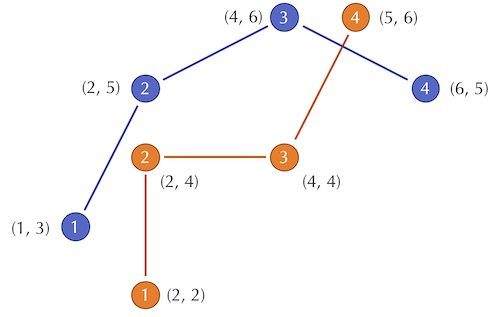
\includegraphics[width = 0.7\textwidth]{../images/rmsd_simple_shapes.png}
	\caption{Two shapes with four points sampled from each.}
	\label{fig:rmsd_simple_shapes}
\end{figure}

\begin{qbox}[%
	Do you see any issues with using RMSD to compare two shapes?
]\end{qbox}

Even if we assume that two shapes have already been overlapped and rotated appropriately, we still should ensure that we sample enough points to give a good approximation of how different the shapes are. Consider a circle inscribed within a square (\autoref{fig:circle_square_undersampling}). If we happened to sample only the four points indicated, then we would sample the same points for each shape and conclude that the RMSD between these two shapes is equal to zero. Fortunately, this issue is easily resolved by making sure to sample enough points from the shape boundaries.\\

\begin{figure}[h]
	\centering
	\mySfFamily
	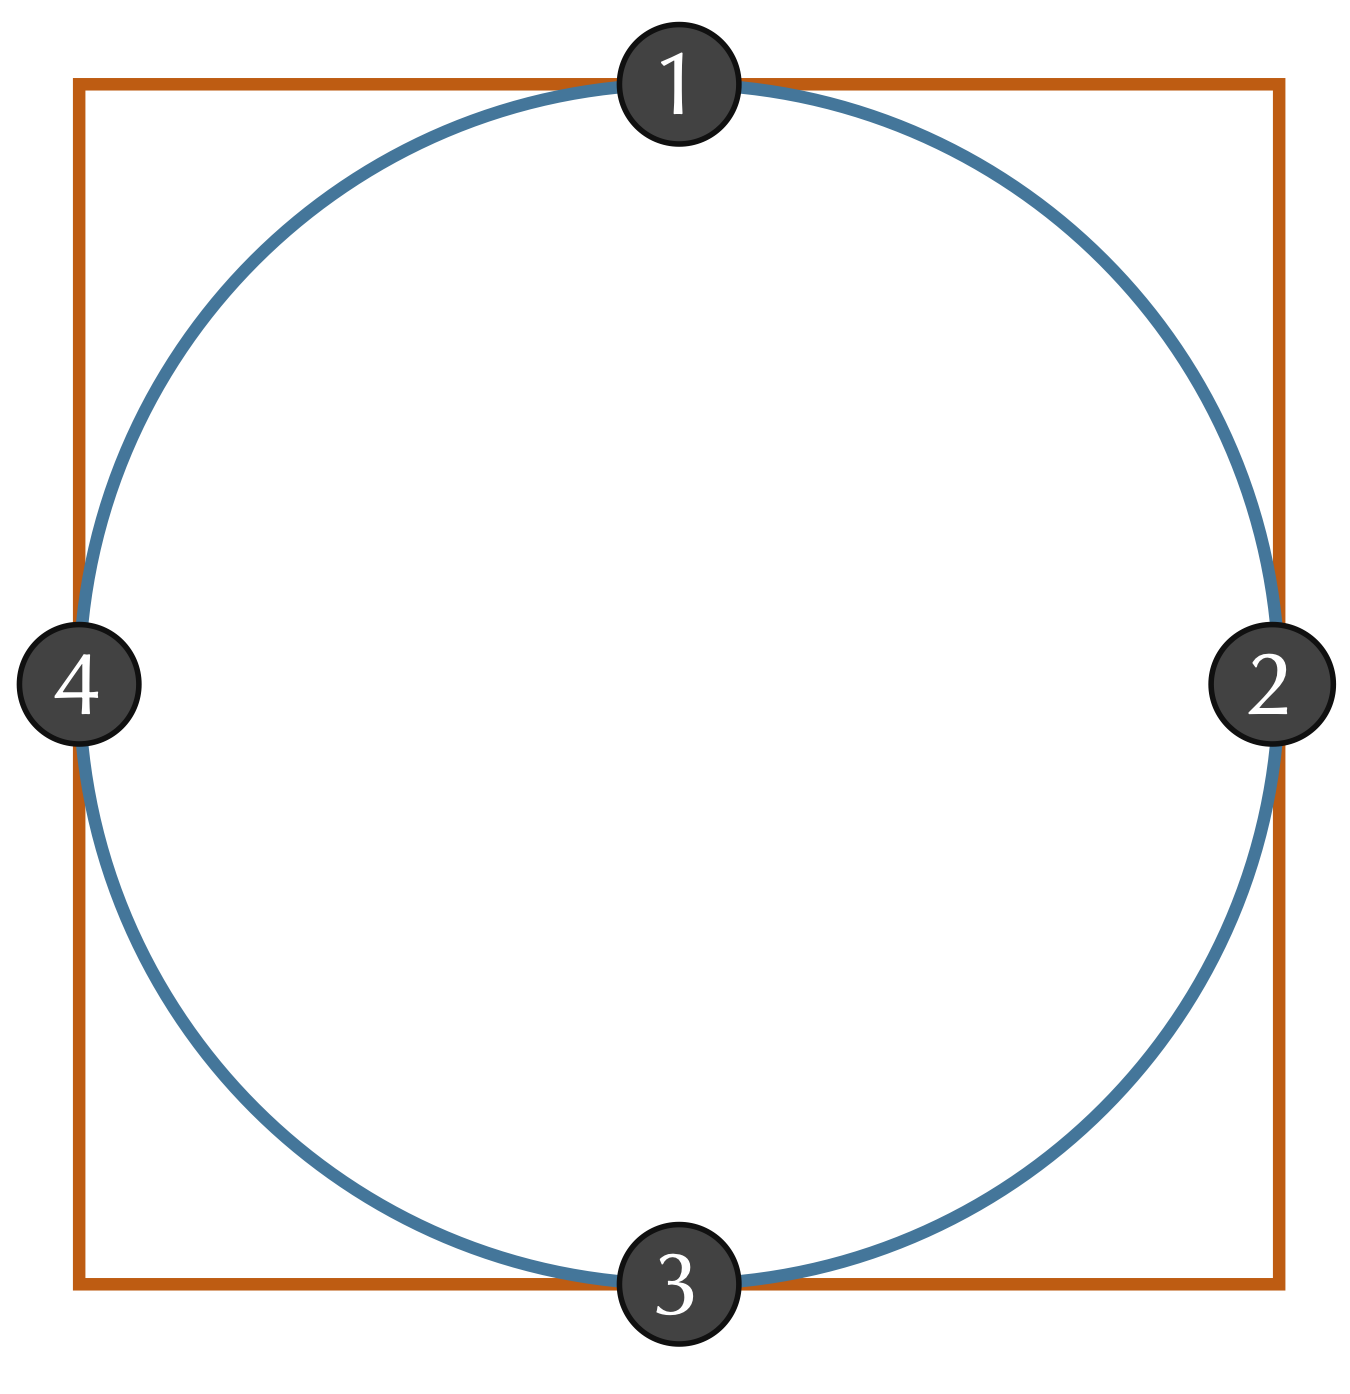
\includegraphics[width = 0.4\textwidth]{../images/circle_square_undersampling.png}
	\caption{A circle inscribed within a square. Sampling of the four points where the shapes intersect will give a flawed estimate of zero for the RMSD.}
	\label{fig:circle_square_undersampling}
\end{figure}

Throughout the above discussion, we have assumed that we already rotated (and possibly flipped) \textit{S} to be as ``similar'' to \textit{T} as possible. In practice, after superimposing \textit{S} and \textit{T} to have the same center of mass, we would like to find the flip and/or rotation of \textit{S} that \textit{minimizes} the RMSD between our vectorizations of \textit{S} and \textit{T} over all possible ways of flipping and rotating \textit{S}; fortunately, this flip and/or rotation can be found with an approach called the \textdef{Kabsch algorithm}{Kabsch algorithm}{an algorithm that identifies the best alignment of two shapes} that relies on some advanced linear algebra and is beyond the scope of this work. After applying the Kabsch algorithm to rotate and/or flip $S$, we set our desired distance $d(S, T)$ equal to the RMSD between the shapes' vectors of sampled points.

\phantomsection
\subsection{PDB format represents a protein's structure}

The Kabsch algorithm offers a compelling way to determine the similarity of two protein structures. We can convert a protein containing \textit{n} amino acids into a vector of length \textit{n} by selecting a single representative point from each amino acid. We typically use the alpha carbon, the amino acid's centrally located carbon atom (recall the chemical structure of an amino acid from \autoref{fig:AminoAcid}).\\

\begin{figure}[h]
\centering
\mySfFamily
\scriptsize
\tabcolsep = 0.4em
\rowcolors{2}{gray!25}{white}
\begin{tabular}{c c c c c c c c c c}
\rowcolor{gray!50}
 & &  &  &  & & & \multicolumn{3}{c}{\textbf{Coordinates}}\\
\rowcolor{gray!50}
 & & \textbf{Index} & \textbf{Element} & \textbf{Amino acid} & \textbf{Chain} & \textbf{Position} & \textit{\textbf{x}} & \textit{\textbf{y}} & \textit{\textbf{z}}\\
\gray{2159} & ATOM & 1 & N & ALA& A & 27 & 171.646& 251.874& 224.877\\
\Green{2160} & \Green{ATOM} & \Green{2} & \Green{CA} & \Green{ALA}& \Green{A} & \Green{27} & \Green{172.298}& \Green{252.181} & \Green{223.613}\\
\gray{2161} & ATOM & 3 & C & ALA& A & 27 & 173.530& 251.298& 223.427\\
\gray{2162} & ATOM & 4 & O & ALA& A & 27 & 174.195& 250.943& 224.405\\
\gray{2163} & ATOM & 5 & CB & ALA& A & 27 & 172.700& 253.664& 223.554\\
\gray{2164} & ATOM & 6 & N & TYR& A & 28 & 173.816& 250.939& 222.166\\ 
\Green{2165} & \Green{ATOM} & \Green{7} & \Green{CA} & \Green{TYR} & \Green{A} & \Green{28} & \Green{174.968} & \Green{250.129} &\Green{221.763}\\
\gray{2166} & ATOM & 8 & C & TYR& A & 28 & 175.652& 250.729& 220.561\\
\gray{2167} & ATOM & 9 & O & TYR& A & 28 & 175.009& 251.379& 219.736\\
\gray{2168} & ATOM & 10 & CB & TYR& A & 28 & 174.546& 248.703& 221.426\\
\gray{2169} & ATOM & 11 & CG & TYR& A & 28 & 174.049& 247.932& 222.586\\
\gray{2170} & ATOM & 12 & CD1& TYR& A & 28 & 172.752& 248.072& 223.009\\
\gray{2171} & ATOM & 13 & CD2& TYR& A & 28 & 174.897& 247.067& 223.225\\
\gray{2172} & ATOM & 14 & CE1& TYR& A & 28 & 172.304& 247.348& 224.080\\
\gray{2173} & ATOM & 15 & CE2& TYR& A & 28 & 174.455& 246.338& 224.291\\
\gray{2174} & ATOM & 16 & CZ & TYR& A & 28 & 173.161& 246.477& 224.723\\
\gray{2175} & ATOM & 17 & OH & TYR& A & 28 & 172.710& 245.746& 225.795
\end{tabular}
\caption{Lines \text{2,159} to \text{2,175} of the \texttt{.pdb} file for the experimentally verified SARS-CoV-2 spike protein structure, PDB entry \href{http://www.rcsb.org/structure/6VXX}{6vxx}. These 17 lines contain information on the atoms taken from two amino acids, alanine and tyrosine. The rows corresponding to these amino acids' alpha carbons are shown in green and appear as ``CA'' under the ``Element'' column.  We have labeled the columns to make it clear what each column corresponds to: ``Index'' refers to the number of the amino acid; ``Element'' identifies the chemical element to which this atom corresponds; ``Chain'' indicates which chain the atom is found on; ``Position'' identifies the position in the protein of the amino acid from which the atom is taken; ``Coordinates'' indicates the \textvar{x}, \textvar{y}, and \textvar{z} coordinates of the atom's location (in angstroms).}
\label{fig:simplifiedPDB}
\end{figure}

Whether a protein structure is experimentally validated or predicted by an algorithm, the structure is often represented in a unified file format used by the PDB called \texttt{.pdb} format (\autoref{fig:simplifiedPDB}). In this format, each atom in the protein is labeled according to several different characteristics, including: the element from which the atom derives; the amino acid in which the atom is contained; the chain on which this amino acid is found; the position of the amino acid within this chain; and the 3D coordinates $(x, y, z)$ of the atom in angstroms ($10^{-10}$ meters).\\

\begin{note}[%
	\autoref{fig:simplifiedPDB} shows just part of the information needed to fully represent a protein structure. For example, a \texttt{.pdb} file will also contain information about the disulfide bonds between amino acids. For more information, consult the \href{http://www.wwpdb.org/documentation/file-format}{official PDB documentation}.
	]\end{note}

\phantomsection
\subsection{The Kabsch algorithm can be fooled}

Although the Kabsch algorithm is powerful, we should be careful when using it. Consider \autoref{fig:RMSD_weakness_mutation}, which shows two toy protein structures; the orange structure (\textit{S}) is identical to the blue structure (\textit{T}) except for a change in a single bond angle between the third and fourth amino acids. And yet this tiny change in the protein's structure causes a significant increase in $d(s_{i}, t_{i})$ for every \textit{i} greater than 3, which inflates the RMSD.

\begin{figure}[p]
	\centering
	\mySfFamily
	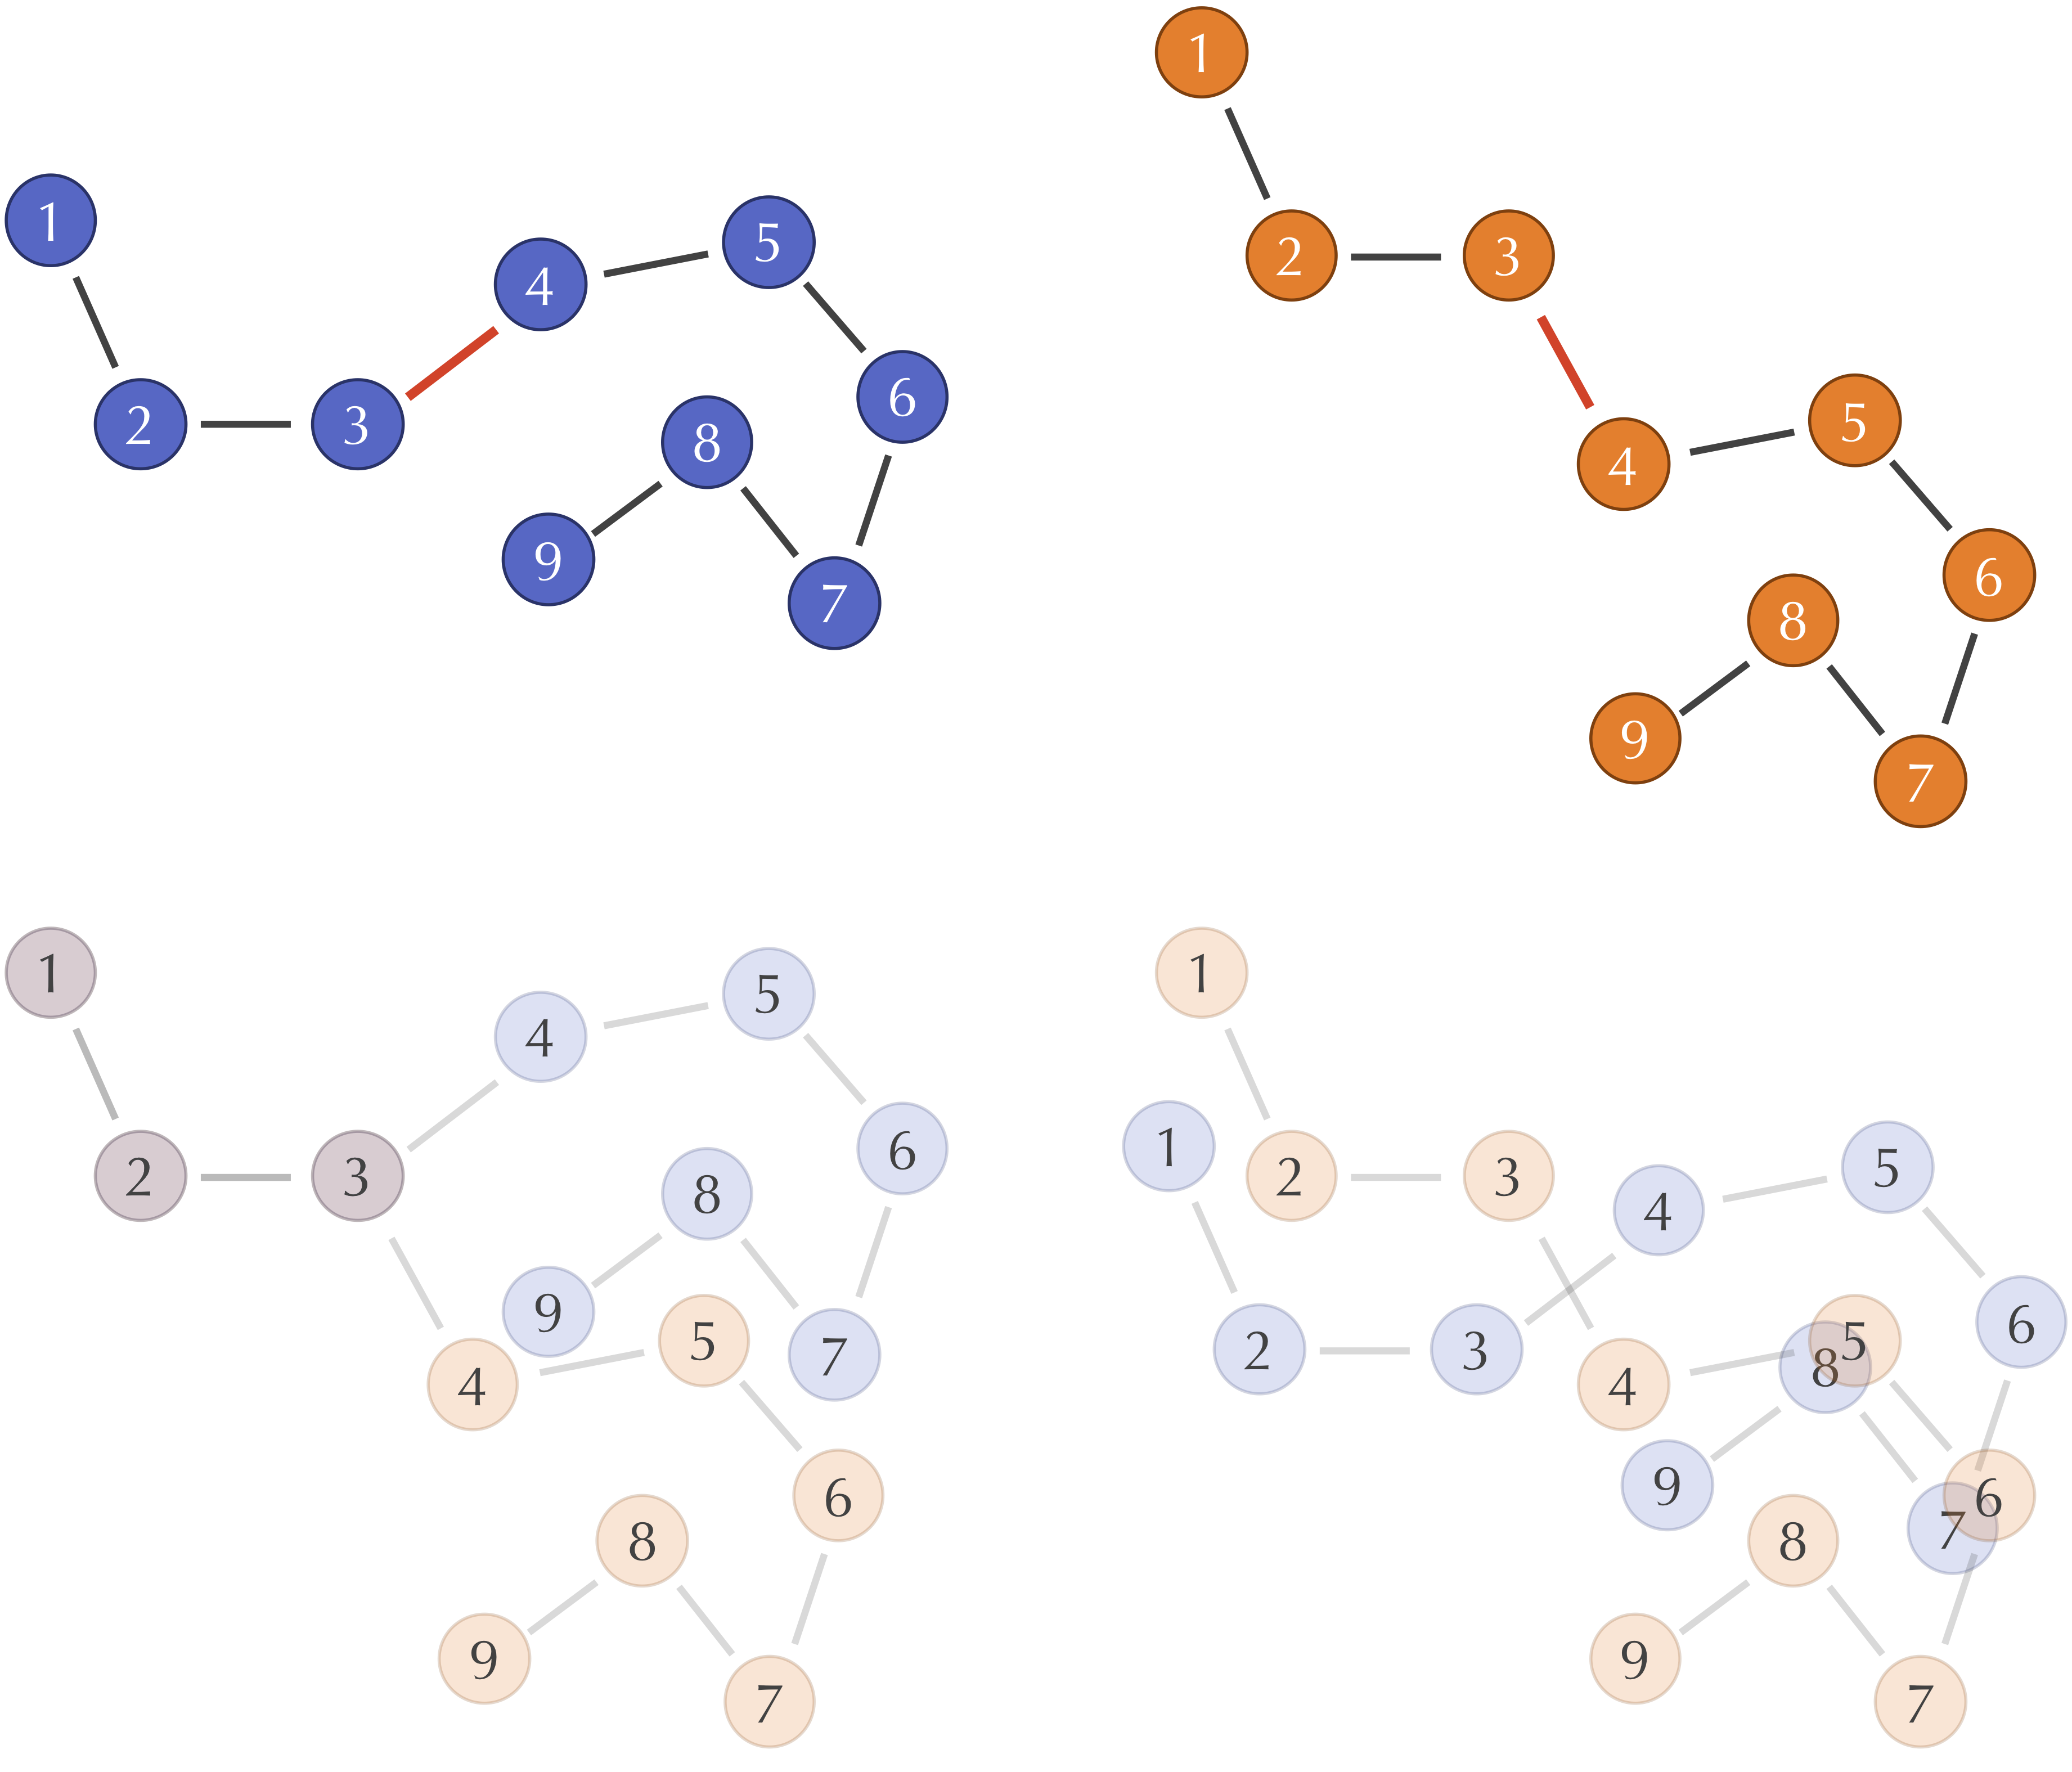
\includegraphics[width = 0.85\textwidth]{../images/RMSD_weakness_mutation.png}
	\caption{(Top) Two hypothetical protein structures that differ in only a single bond angle between the third and fourth amino acids, shown in red. Each circle represents an alpha carbon. (Bottom left) Superimposing the first three amino acids shows how much the change in the bond angle throws off the computation of RMSD by increasing the distances between corresponding alpha carbons. (Bottom right) The Kabsch algorithm would align the centers of gravity of the two structures in order to minimize RMSD between corresponding alpha carbons. This alignment belies the similarity in the structures and makes it difficult for the untrained observer to notice that the two proteins only differ in a single bond angle.}
	\label{fig:RMSD_weakness_mutation}
\end{figure}

Another way in which the Kabsch algorithm can be tricked is in the case of an appended substructure that throws off the ordering of the amino acids. \autoref{fig:RMSD_weakness_loop} shows a toy example of a structure into which we incorporate a loop, thus throwing off the natural order of comparing amino acids. (The same effect is caused if one or more amino acids are deleted from one of the two proteins.)

\begin{figure}[t]
	\centering
	\mySfFamily
	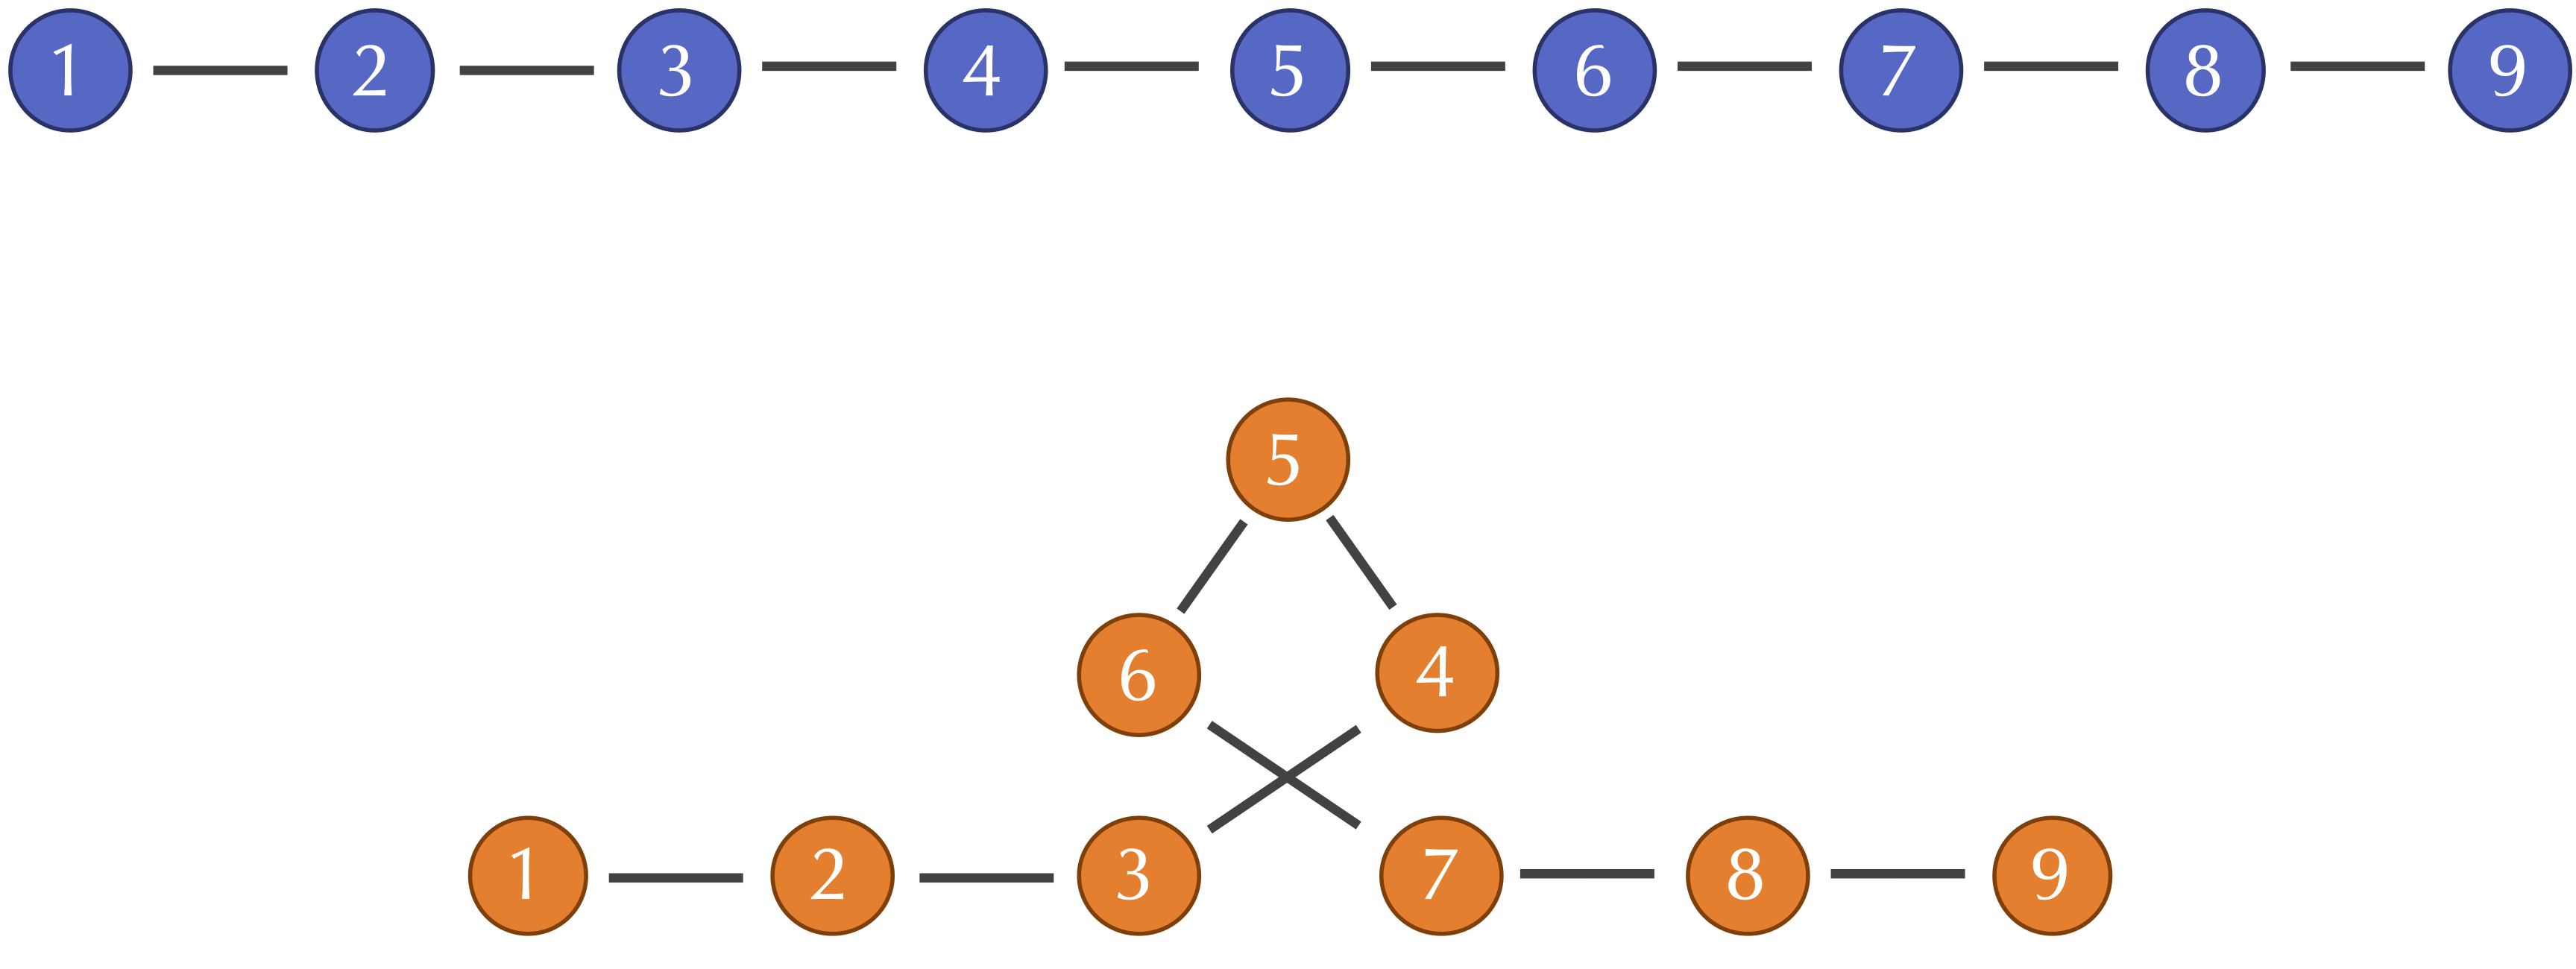
\includegraphics[width = 0.7\textwidth]{../images/RMSD_weakness_loop.png}
	\caption{Two toy protein structures, one of which (bottom) includes a loop of three amino acids. After the loop, each amino acid in the orange structure will be compared against an amino acid that occurs farther long in the blue structure, thus increasing $\textvar{d}(\textvar{s}_{\textvar{i}}, \textvar{t}_{\textvar{i}})$ for each such amino acid and inflating RMSD.}
	\label{fig:RMSD_weakness_loop}
\end{figure}

To address this second issue, biologists will often align the sequences of two proteins first, discarding any positions that do not align well when it comes time to perform the RMSD calculation. We will soon see an example of a protein sequence alignment when comparing the coronavirus spike proteins.

In short, if the RMSD of two proteins is \textit{large}, then we should be wary of concluding that the proteins are very different, and we may need to combine RMSD with other methods of structure comparison. But if the RMSD is \textit{small} (e.g., just a few angstroms), then we can have confidence that the proteins are indeed similar.

We are now ready to apply the Kabsch algorithm to compare the structures that we predicted for human hemoglobin subunit alpha and the SARS-CoV-2 spike protein against their experimentally validated structures. \tutorial[coronavirus/tutorial_rmsd]

\FloatBarrier
\phantomsection
\subsection{Assessing the accuracy of our structure prediction models}

Earlier in this chapter, we used publicly available protein structure prediction servers to predict the structure of human hemoglobin subunit alpha (using \textit{ab initio} modeling) and the SARS-CoV-2 spike protein (using homology modeling). We will now see how well our models performed by showing the values of RMSD produced by the Kabsch algorithm when comparing each of these models against the validated structures.

\autoref{fig:quark_rmsd_table} shows the RMSD between each of the five predicted structures returned by QUARK and the validated structure of human hemoglobin subunit alpha. We are tempted to conclude that our \textit{ab initio} prediction was a success. However, because human hemoglobin subunit alpha is so short (141 amino acids), researchers would consider this RMSD score to be high.\fudgespace

\begin{figure}[h]
	\centering
	\tabcolsep = 1 em
	\mySfFamily
	\begin{tabular}{c c}
		\textbf{QUARK Models} & \textbf{RMSD} \\
		QUARK 1 & 1.58\phantom{xx} \\
		QUARK 2 & 2.0988\\
		QUARK 3 & 3.11\phantom{xx} \\
		QUARK 4 & 1.9343\\
		QUARK 5 & 2.6495
	\end{tabular}
	\caption{The RMSD of five models of human hemoglobin subunit alpha predicted by QUARK compared against the protein's validated structure (PDB entry: \href{https://www.rcsb.org/structure/1si4}{1si4}).}
	\label{fig:quark_rmsd_table}
\end{figure}


\FloatBarrier
\phantomsection
\subsection{Homology models of the SARS-CoV-2 spike protein}

We also used GalaxyWeb to predict the structure of the SARS-CoV-2 spike protein's RBD, Robetta to predict the structure of a single chain, and SWISS-MODEL to predict the structure of the entire protein. \autoref{fig:sars-cov-2_rmsd_table} compiles the RMSD of structures predicted by this homology modeling software against experimental results.\\

\begin{figure}[h]
	\centering
	\tabcolsep = 1 em
	\mySfFamily
	\begin{tabular}{c c}
		\textbf{Predicted Structure} & \textbf{RMSD} \\
		GalaxyWEB 1 & \phantom{x}0.1775 \\
		GalaxyWEB 2 & \phantom{x}0.1459 \\
		GalaxyWEB 3 & \phantom{x}0.1526 \\
		GalaxyWEB 4 & \phantom{x}0.1434 \\
		GalaxyWEB 5 & \phantom{x}0.1202 \\
		Robetta 1 & \phantom{x}3.1189 \\
		Robetta 2 & \phantom{x}3.7568 \\
		Robetta 3 & \phantom{x}2.9972 \\
		Robetta 4 & \phantom{x}2.5852 \\
		Robetta 5 & 12.0975 \\
		SWISS-Model 1 & \phantom{x}5.8518 \\
		SWISS-Model 2 & 11.3432 \\
		SWISS-Model 3 & 11.3432 \\
	\end{tabular}
	\caption{A table containing the RMSD of SARS-CoV-2 spike protein structures predicted by software against the known structure. GalaxyWEB's results are compared against the RBD (PDB entry: \href{https://www.rcsb.org/structure/6lzg}{6lzg}); Robetta's results are compared against a single chain, and SWISS-Model's are compared against the entire protein (PDB entry: \href{https://www.rcsb.org/structure/6vxx}{6vxx}).}
	\label{fig:sars-cov-2_rmsd_table}
\end{figure}

The GalaxyWEB models have an excellent RMSD score and can be considered very accurate. Note that their RMSD is more than an order of magnitude lower than the RMSD computed for our \textit{ab initio} predictions of hemoglobin subunit alpha, despite the fact that the RBD is longer (229 amino acids). As for the other two software resources, although the RMSD values are higher than those of GalaxyWEB, keep in mind that a single chain of the spike protein is 1,281 amino acids long, and so the sensitivity of RMSD to slight changes should give us confidence that our models are on the right track.\\

\begin{qbox}[%
	Which do you think performed more accurately on our predictions: SWISS-MODEL or Robetta?
]\end{qbox}

\phantomsection
\subsection{Distributing the work of protein structure prediction around the world}

Two leading structure prediction projects, \href{https://boinc.bakerlab.org}{Rosetta@home} and \href{https://foldingathome.org}{Folding@home}, encourage volunteers to download their software and contribute to a gigantic \textit{distributed} effort to predict protein shape. Even with a modest laptop, a user can donate some of their computer's idle resources to contribute to the problem of protein structure prediction. While some researchers were working to elucidate the structure of the SARS-CoV-2 spike protein experimentally, thousands of users were devoting their computers to the cause of predicting the protein's structure computationally.

The RMSD values for the models predicted by Rosetta@Home are shown in \autoref{fig:ssgcid_rmsd_table}. As we might expect due to having access to thousands of users' computers, these models outperform our own from \autoref{fig:sars-cov-2_rmsd_table}. Yet a typical threshold for whether a predicted structure is accurate is if its RMSD compared to a validated structure is smaller than 2.0 angstroms, a test that the models in \autoref{fig:ssgcid_rmsd_table} do not pass.

\begin{figure}[h]
	\centering
	\tabcolsep = 1 em
	\mySfFamily
	\begin{tabular}{c c c}
		\textbf{Rosetta@Home Models} & \textbf{RMSD (Single Chain)} & \textbf{RMSD (Full Protein)}\\
		Model 1  & 2.7843 & 3.505\phantom{x}  \\
		Model 2  & 2.107\phantom{x} & 2.3274 \\
		Model 3  & 1.866\phantom{x} & 2.12\phantom{xx} \\
		Model 4  & 2.047\phantom{x} & 2.0854 \\
		Model 5  & 4.6443 & 4.9636
	\end{tabular}
	\caption{A table containing the the calculated RMSD of the Rosetta@Home models of SARS-CoV-2 spike protein, full protein and single chain, compared to the validated structure (PDB entry: 6vxx).}
	\label{fig:ssgcid_rmsd_table}
\end{figure}

The inability of even powerful models to obtain an accurate predicted structure may make it seem that protein structure prediction is a lost cause. Perhaps biochemists should head back to expensive experimental validations and ignore the musings of computational scientists. In the conclusion to this chapter, we will find hope.\\

\FloatBarrier
\phantomsection

\section{Conclusion: Protein Structure Prediction is Solved?}
\label{sec:conclusion_part_1}
\phantomsection

Protein structure prediction is an old problem. In 1967, the Soviets founded an entire research institute dedicated to solving ``the protein problem''; this institute still lives on today. Despite the difficulty of protein structure prediction, gradual algorithmic improvements and increasing computational resources have led biologists around the world to wish for the day when they could consider protein structure prediction to be solved.

That day has come. Kind of.

Every two years since 1994, a global contest called \textdefnogloss{Critical Assessment of protein Structure Prediction (CASP)} has allowed modelers to test their protein structure prediction algorithms against each other. The contest organizers compile a (secret) collection of experimentally verified protein structures and then run all submitted algorithms against these proteins.

In 2020, the 14th iteration of this contest (CASP14) was won in a landslide. The second version of \href{https://bit.ly/3sKl6pH}{\textdefnogloss{AlphaFold}}, a DeepMind project, vastly outperformed the world's foremost structure prediction approaches. The algorithm powering AlphaFold is an extremely involved method based on deep learning, a topic that we will touch upon in \autoref{chapter:white_blood_cells}.

Instead of using RMSD, CASP scores a predicted structure against a known structure using the \textdefnogloss{global distance test (GDT)}. We first ask, ``How many corresponding alpha carbons are close to each other in the two structures?'' To answer this question, we take the percentage of corresponding alpha carbon positions having distance apart that is at most equal to some threshold \textit{t}. The GDT score averages the percentages obtained when \textit{t} is equal to each of 1, 2, 4, and 8 angstroms. A GDT score of 90\% is considered good, and a score of GDT 95\% is considered excellent (i.e., comparable to minor errors resulting from experimentation).

We will show a few plots to illustrate the decisiveness of AlphaFold's CASP14 victory. In \autoref{fig:AlphaFold2_BAKER_Zhang} (top), we compare the GDT scores of AlphaFold against the second-place algorithm (a product of David Baker's laboratory, which developed the Robetta and Rosetta@Home software that we encountered in this chapter). We can appreciate the size of this margin of victory if we compare it against the difference between the second and third place competitors (\autoref{fig:AlphaFold2_BAKER_Zhang} (bottom)).

\begin{figure}[h]
	\centering
	\mySfFamily
	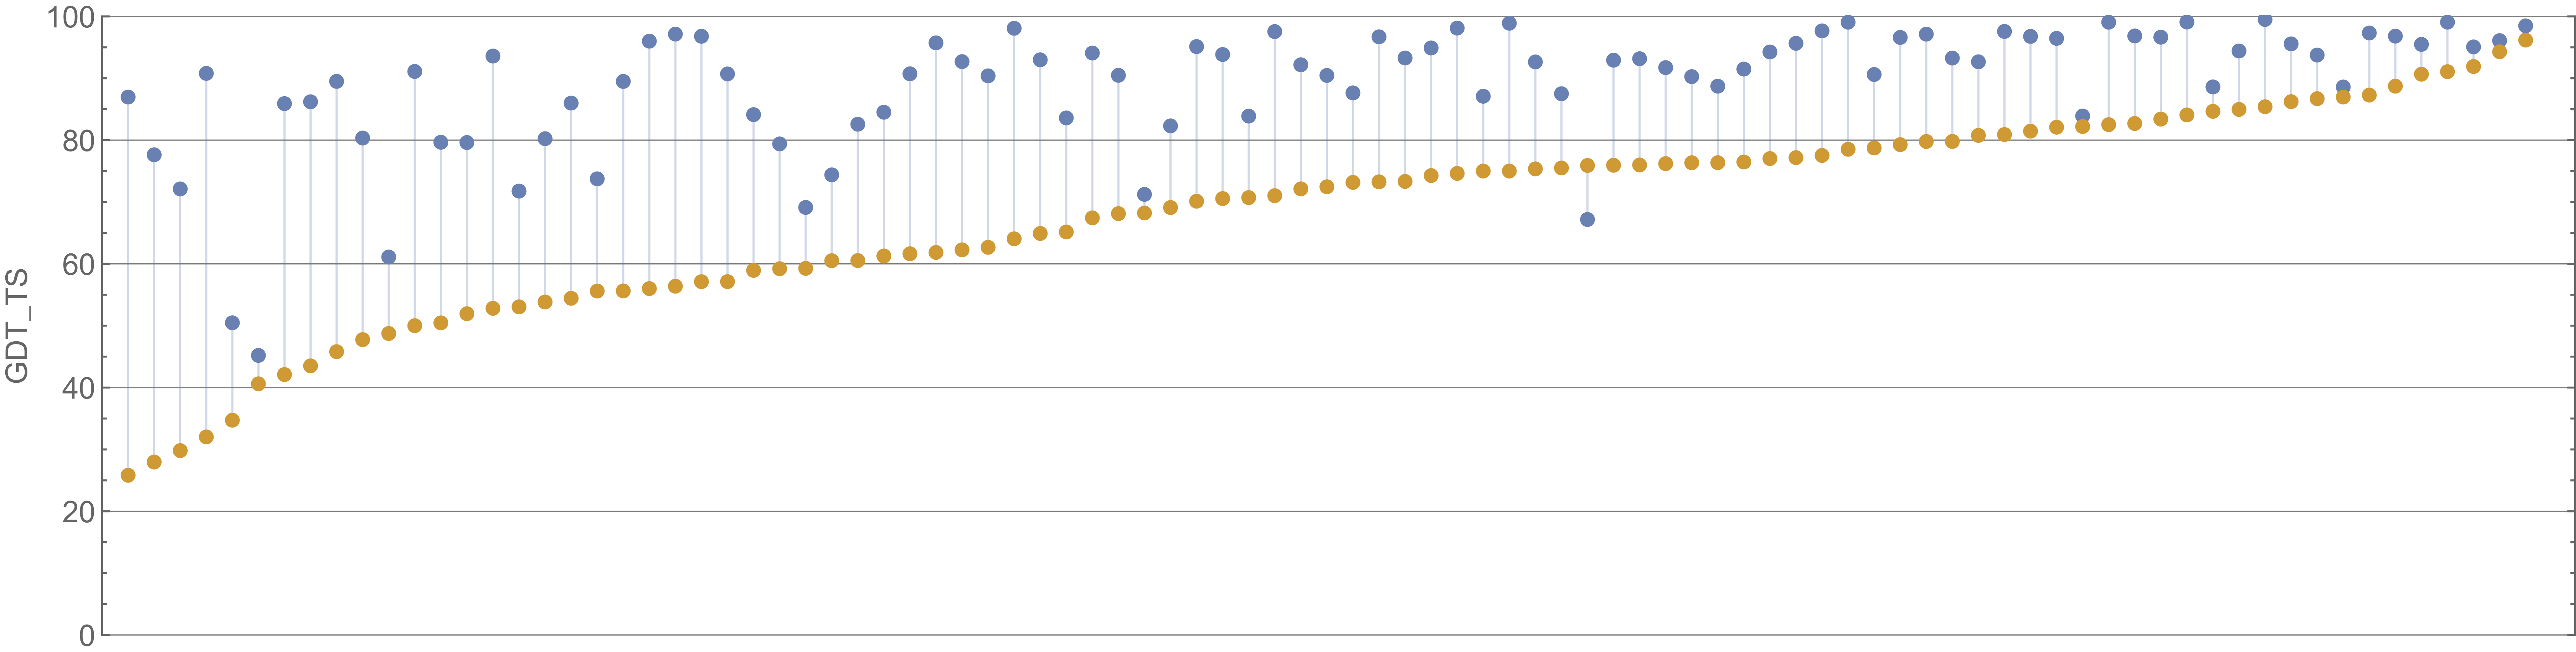
\includegraphics[width = 0.85\textwidth]{../images/AlphaFold2_BAKER.png}\\[4ex]
	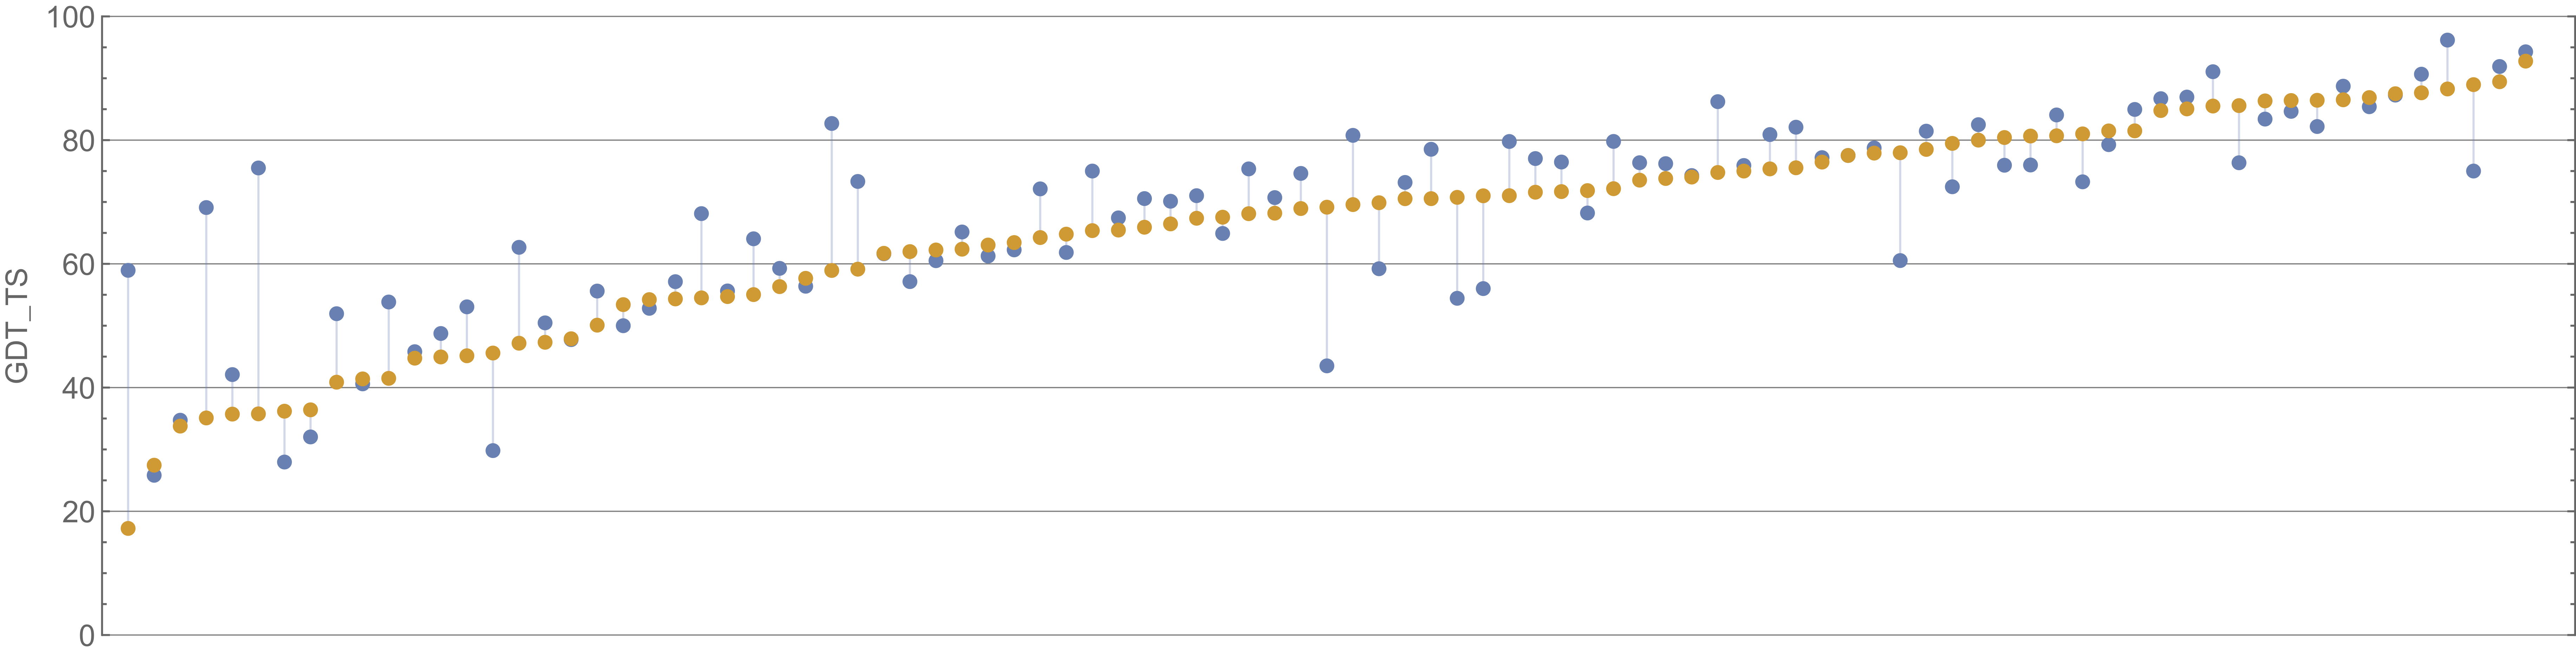
\includegraphics[width = 0.85\textwidth]{../images/BAKER_Zhang.png}
	\caption{(Top) A plot of GDT scores for the AlphaFold2 (blue) and Baker lab (orange) submissions over all proteins in the CASP14 contest. AlphaFold2 finished first in CASP14, and Baker lab finished second. (Bottom) A plot of GDT scores for the Baker lab (blue) and Zhang lab (orange) submissions for all proteins in the CASP14 contest. Zhang lab finished third in CASP14.}
	\label{fig:AlphaFold2_BAKER_Zhang}
\end{figure}

For each protein in the CASP14 contest, we can also compute each algorithm's \textdefnogloss{z-score}, defined as the number of standard deviations that the algorithm's GDT score falls from the mean GDT score over all competitors. For example, a z-score of 1.4 would imply that the approach performed 1.4 standard deviations above the mean, and a z-score of $-0.9$ would imply that the approach performed 0.9 standard deviations below the mean.

By summing all of an algorithm's positive z-scores, we obtain a reasonable metric for the relative quality of an algorithm compared to its competitors. If this sum of z-scores is large, then the algorithm racked up lots of positive z-scores, meaning that it is performing significantly above average on the prediction of some proteins. \autoref{fig:CASP14_overall_results} shows the sum of z-scores for all CASP14 participants and reiterates the margin of AlphaFold's victory, since its sum of z-scores was twice that of the second place algorithm.

\begin{figure}[h]
	\centering
	\mySfFamily
	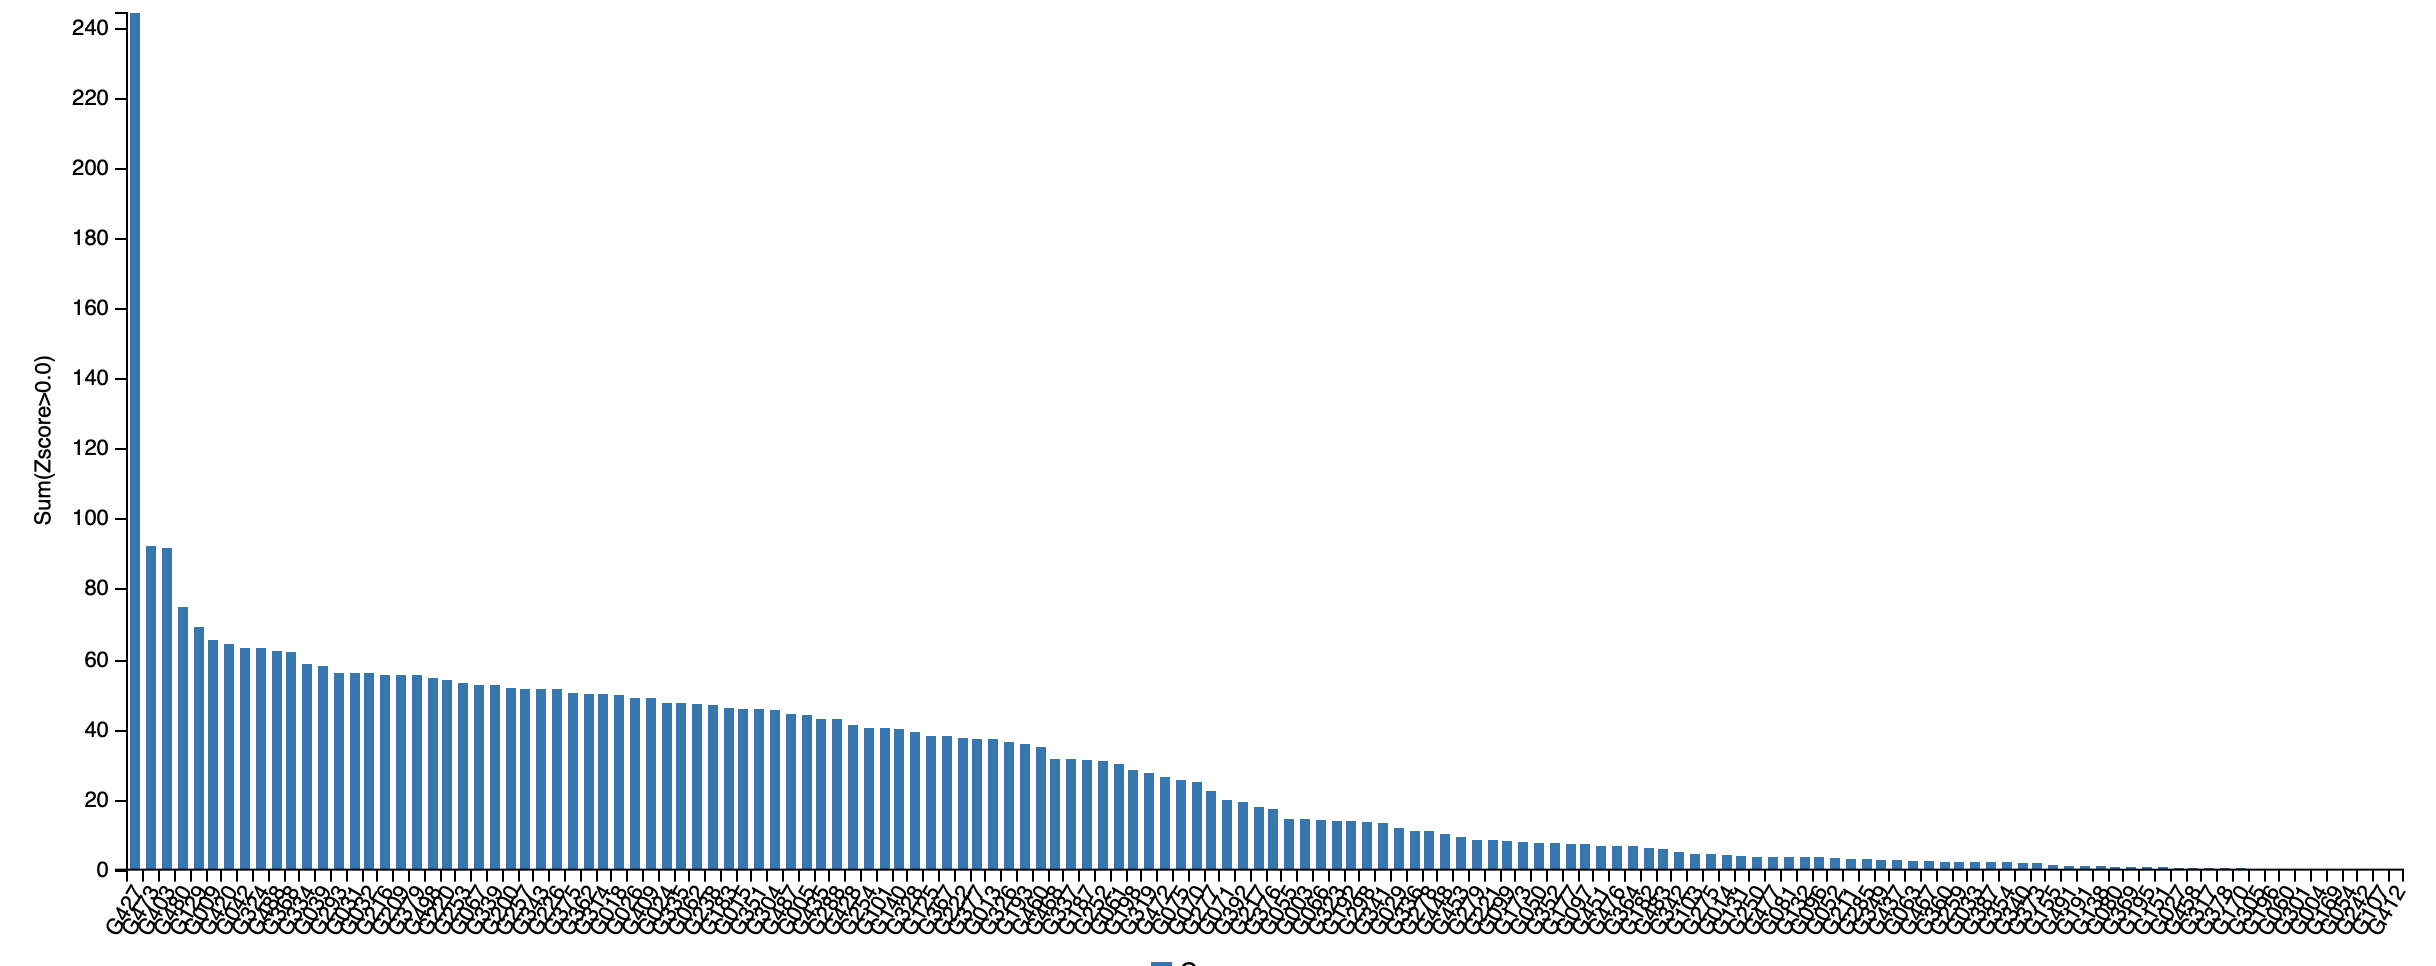
\includegraphics[width = 0.85\textwidth]{../images/CASP14_overall_results.png}
	\caption{A bar chart plotting the sum of z-scores for every entrant in the CASP14 contest. AlphaFold2 is shown on the far left; its sum of z-scores is over double that of the second-place submission.}
	\label{fig:CASP14_overall_results}
\end{figure}

AlphaFold's CASP14 triumph led some scientists --- and media outlets --- to declare that protein structure prediction had finally been solved. Yet some critics remained skeptical.

Although AlphaFold obtained an impressive median RMSD of 1.6 angstroms for its predicted proteins, about a third of these predictions have an RMSD over 2.0 angstroms, which we mentioned earlier is often used as a threshold for whether a predicted structure is reliable. We will not know in advance whether AlphaFold's predicted structure is outside of this range unless we experimentally validate the protein's structure.

Furthermore, some experts have claimed that to be completely trustworthy for a sensitive application like designing drugs to target proteins implicated in diseases, the RMSD of predicted protein structures would need to be nearly an order of magnitude lower, i.e., closer to 0.2 angstroms.

Finally, the AlphaFold algorithm is ``trained'' using a database of known protein structures, which makes it more likely to succeed if a protein is similar to a known structure. But the proteins with structures that are \textit{dissimilar} to any known structure are the ones possessing some of the greatest scientific interest.

Pronouncing protein structure prediction to be solved may be hasty, but we will likely never again see such a clear improvement to the state of the art for structure prediction. AlphaFold represents, perhaps, the final great innovation for a research problem that has puzzled biologists for over half a century.

Thus ends our discussion of protein structure prediction, but we still have much more to say. In particular, when comparing two protein structures, we have relied only upon the RMSD between the vectorizations of these two structures after applying the Kabsch algorithm. But using a single statistic to represent the differences between two protein structures belies what those differences might be. Furthermore, proteins are not static objects; they bend and shape in their environment as they perform their tasks. We will therefore now transition into a second part of our treatment of protein analysis, in which we show additional methods used to compare proteins and apply these techniques to the validated structures of the SARS-CoV and SARS-CoV-2 spike proteins.

\newpage

\FloatBarrier
\phantomsection

\section{Exercises}

\phantomsection
\subsection{Determining a shape's center of mass mathematically}

In the main text, we noted that the center of some shapes can be computed mathematically. Consider the semicircular arc shown in \autoref{fig:semicircular_arc}, with endpoints $(-1, 0)$ and $(1, 0)$.\\

%The \textit{x}-coordinate $x_{S}$ is zero, but computing $y_{S}$ requires us to apply a little calculus, taking the average of the \textit{y}-coordinates along the entire semicircle:
%\begin{align*}
%	y_S &= \dfrac{\int_{0}^{\pi}{\sin{\theta}}}{\pi} \\
%	&= \dfrac{-\cos{\pi} + \cos{0}}{\pi} \\
%	&= \dfrac{2}{\pi}
%\end{align*}

\begin{figure}[h]
	\centering
	\mySfFamily
	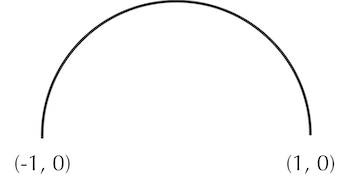
\includegraphics[width = 0.4\textwidth]{../images/semicircular_arc.png}
	\caption{A semicircular arc with radius 1 corresponding to a circle whose center is at the origin.}
	\label{fig:semicircular_arc}
\end{figure}

\begin{exercise}[%
Determine the center of mass of the shape in \autoref{fig:semicircular_arc}. (Hint: finding the x-coordinate of the center of mass is easy, but finding the y-coordinate requires a little calculus for finding an average value.)
]\end{exercise}

\begin{exercise}[%
	Say that we connect $(-1, 0)$ and $(0, 1)$ to form a closed semicircle. What will be the center of mass of the resulting shape?
]\end{exercise}

\phantomsection
\subsection{Calculating RMSD}

Consider the two (very) hypothetical protein structures shown in \autoref{fig:rmsd_exercise} with vectorizations of eight points each.\\

\begin{figure}[h]
	\centering
	\mySfFamily
	\tabcolsep = 2em
	\begin{tabular}{c c}
	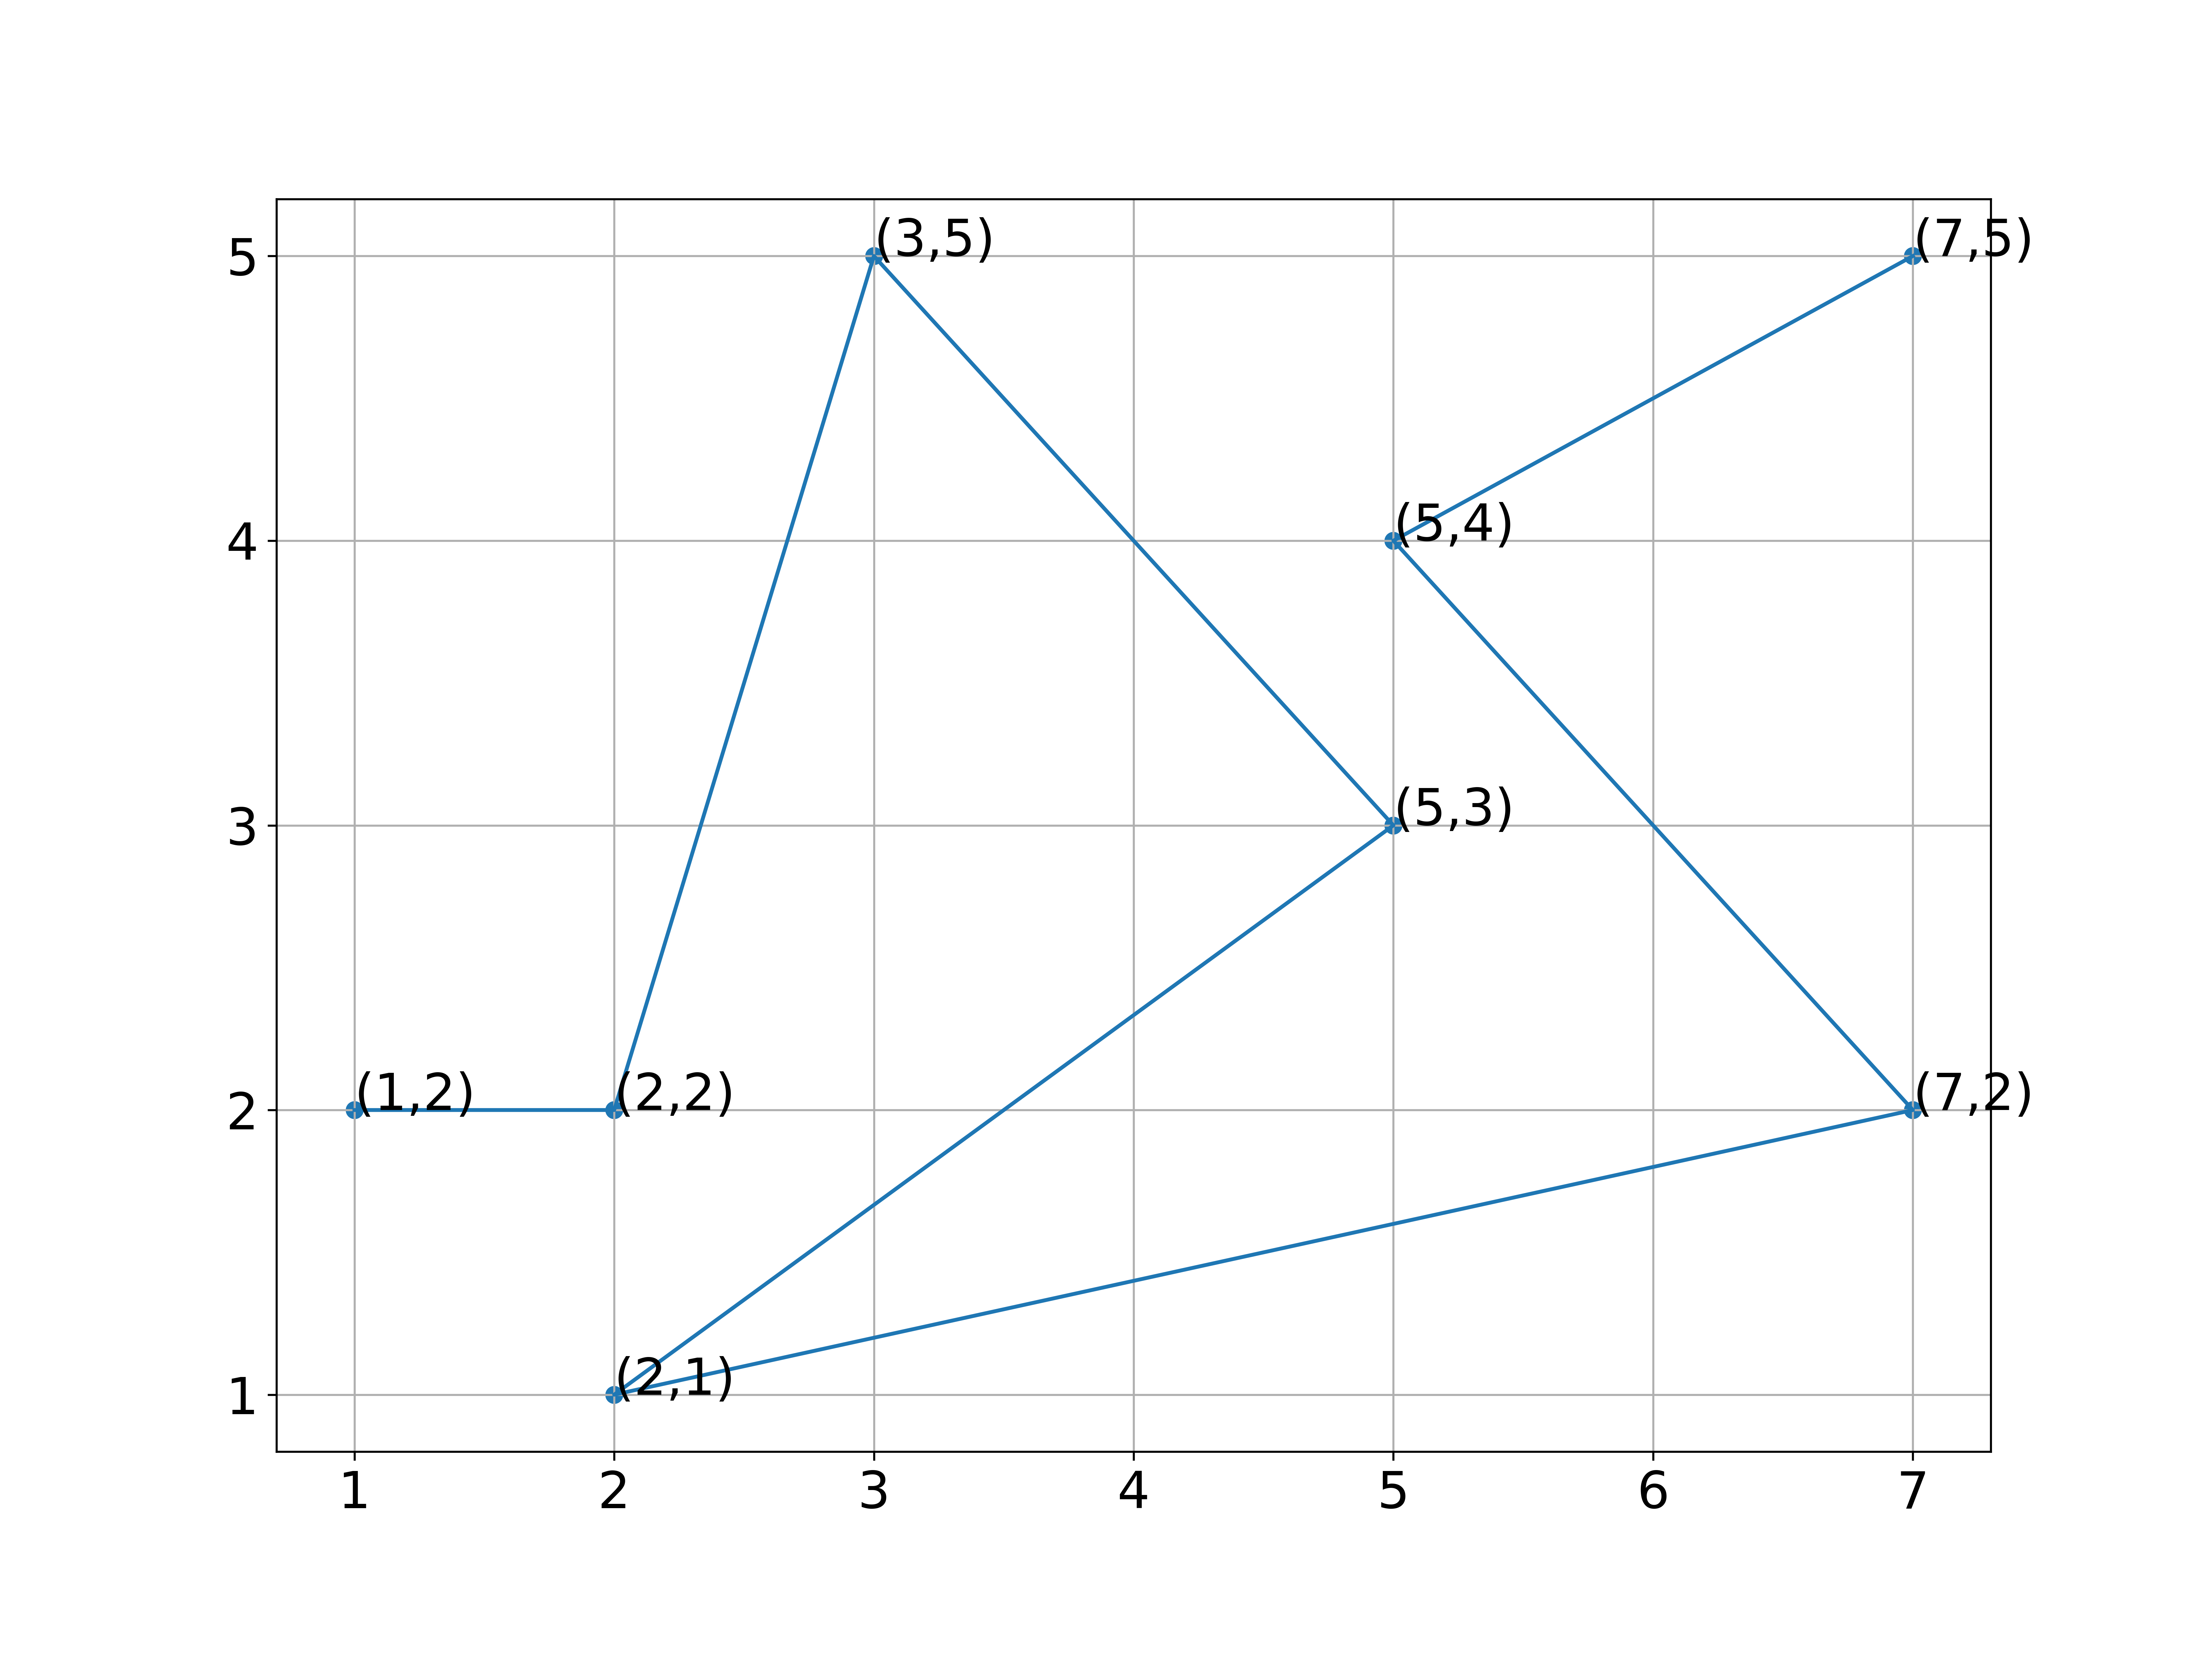
\includegraphics[width = 0.4\textwidth]{../images/rmsd_exercise1.png} & 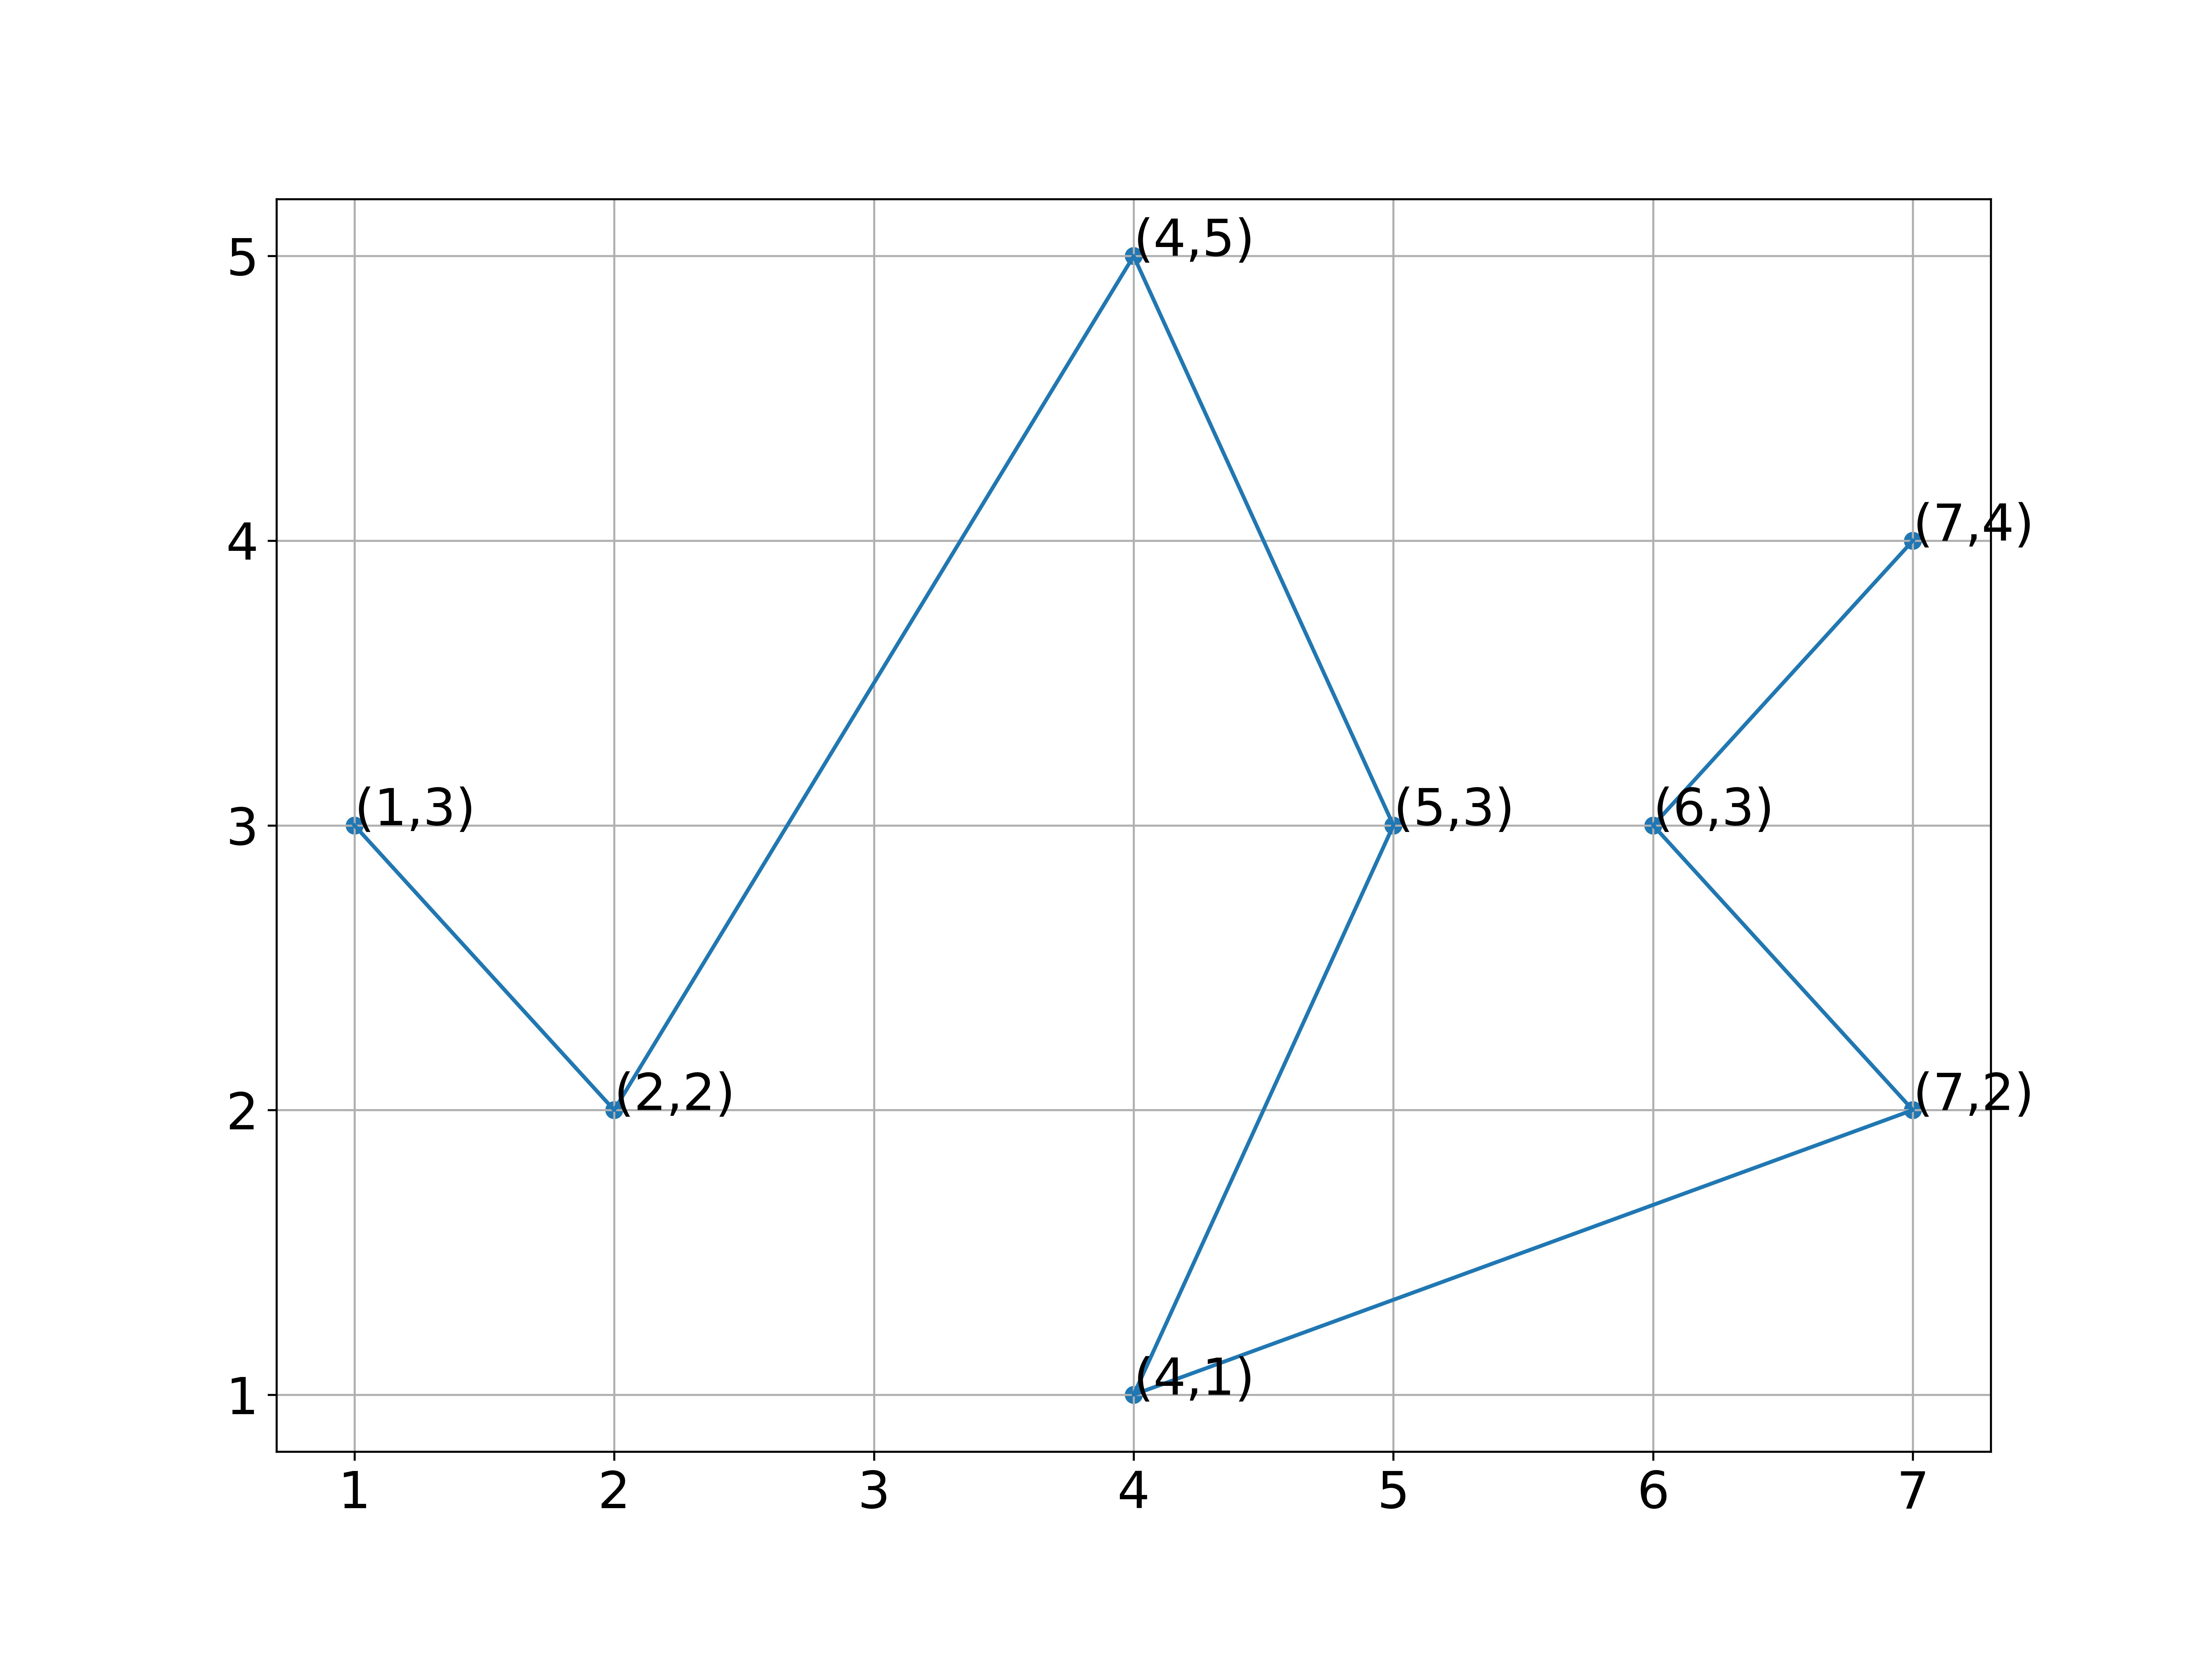
\includegraphics[width = 0.4\textwidth]{../images/rmsd_exercise2.png}
	\end{tabular}
	\caption{Two hypothetical protein structures with vectorizations into eight points each.}
	\label{fig:rmsd_exercise}
\end{figure}

\begin{exercise}[%
Using the vectorization of the figures indicated, estimate the center of mass of these two protein structures.
]\end{exercise}

\begin{exercise}[%
Without rotating these structures, align the two structures in \autoref{fig:rmsd_exercise} so that they have the same center of mass, and determine the RMSD between the two structures for the vectorizations shown.
]\end{exercise}

\phantomsection
\subsection{\textit{Ab initio} and homology modeling}

In this exercise, we will perform \textit{ab initio} and homology structure prediction on a simple protein, the human hemoglobin subunit alpha that we have worked with in this chapter. First, go to the \href{https://www.rcsb.org/}{protein data bank} and search for the protein ``1SI4''. Download the PDB file by clicking on ``Download Files'' and then ``PDB Format''. We will use this file for structure comparisons later. Next, go to the ``Sequence'' tab and click ``Display Files'' and then ``FASTA Sequence''. Copy the first sequence corresponding to the alpha subunit and submit it to the ab initio structure prediction software \href{https://zhanggroup.org/QUARK/}{QUARK}, and your choice of homology modeling software: \href{https://swissmodel.expasy.org/}{SWISS-MODEL}, \href{https://robetta.bakerlab.org/}{Robetta}, or \href{https://galaxy.seoklab.org/cgi-bin/submit.cgi?type=TBM}{GalaxyWEB}. Once you get the results, use ProDy to calculate the RMSD between the predicted structures and the actual structure (1SI4).\\

\begin{exercise}[%
Which type of modeling resulted in the most accurate prediction? Is this what you expected? (\textbf{Hint:} Use ``Chain A'' to focus on subunit alpha.)
]\end{exercise}

\phantomsection
\subsection{Trying out AlphaFold}

In the conclusion of this chapter, we introduced AlphaFold from DeepMind that won the 14th CASP contest in 2020 by a wide margin. A simplified version of AlphaFold is available on Colab. This version currently does not work with the entire spike protein, so we will use the human hemoglobin subunit alpha once again. Following the directions from the previous exercise, grab the protein sequence of the alpha subunit. Next, open the \href{https://colab.research.google.com/github/deepmind/alphafold/blob/main/notebooks/AlphaFold.ipynb#scrollTo=woIxeCPygt7K}{simplified version of AlphaFold}. Read the documentation and follow the directions in each step to generate the predicted structure.\\

\begin{exercise}[%
Use ProDy to calculate the RMSD between the predicted structure and the actual structure (1SI4). Did this simplified version of AlphaFold perform better than your \textit{Ab initio} and homology modeling results from the previous exercise?
]\end{exercise}
